\documentclass[12pt]{article}
\usepackage{amsmath,amssymb,amsthm,bm,enumitem,mathtools}
\usepackage{geometry,graphicx,subcaption,sidecap,multirow}
\geometry{margin = 1 in}
\usepackage{color}

\renewcommand{\arraystretch}{1.5}	% Change of table scale factor

% Discrete notation:
\newcommand{\aVec}{\mathbf{a}}	% Vector
\newcommand{\bVec}{\mathbf{b}}	% Vector
\newcommand{\dVec}{\mathbf{d}}	% Vector
\newcommand{\kVec}{\mathbf{k}}	% Vector
\newcommand{\pVec}{\mathbf{p}}	% Vector
\newcommand{\rVec}{\mathbf{r}}	% Vector
\newcommand{\fVec}{\mathbf{f}}	% Vector
\newcommand{\xVec}{\mathbf{x}}	% Vector
\newcommand{\xTrue}{\mathbf{x}_{\text{true}}}	% Vector (true solution)
\newcommand{\yVec}{\mathbf{y}}	% Vector
\newcommand{\tVec}{\mathbf{t}}	% Vector
\newcommand{\uVec}{\mathbf{u}}	% Vector
\newcommand{\wVec}{\mathbf{w}}	% Vector
\newcommand{\trans}[1]{{#1}^\mathsf{T}}	% Matrix transpose
\newcommand{\ctrans}[1]{{#1}^\mathsf{H}}	% Hermitian transpose
\newcommand{\inv}[1]{{#1}^{-1}}	% Inverse of a matrix
\newcommand{\pinv}[1]{{#1}^\dagger}	% Inverse of a matrix
\DeclareMathOperator{\trace}{trace}		% Trace
\DeclareMathOperator{\diag}{diag}	% Diagonal matrix
\DeclareMathOperator{\rank}{rank}	% Rank of a matrix
\DeclareMathOperator{\range}{range}	% Range (space) of a matrix
\DeclareMathOperator{\nullspace}{null}	% Null (space) of a matrix
\DeclareMathOperator{\proj}{proj}	% Projection
\DeclareMathOperator{\pdet}{det^\dagger}	
\DeclareMathOperator{\sgn}{sgn}	% Signum function
\DeclareMathOperator{\alias}{A}	% Aliasing operator
\newcommand{\dct}[1]{\breve{#1}}	% DCT of vector
\newcommand{\dft}[1]{\widehat{#1}}	% DFT of vector
\DeclareMathOperator{\vcat}{vcat}	% Concatenation of vector
\DeclareMathOperator{\shift}{\sigma}	% Shift operator

% Regularization notation:
\newcommand{\regparam}{\alpha}  % Regularization parameter
\newcommand{\regparamVec}{\mathbf{\regparam}}   % Vector of regularization parameters
\newcommand{\R}{R_{\regparam}}	% Regularization matrix
\newcommand{\regf}{\fVec_{\regparam}}	% Regularized solution
\newcommand{\xReg}{\xVec(\regparam)}	% Regularized solution
\newcommand{\xWin}{\xVec_{\text{win}}(\regparam)}	% Windowed regularized solution
\newcommand{\xSol}{\xVec}	% True solution
\DeclareMathOperator*{\argmax}{arg\,max}
\DeclareMathOperator*{\argmin}{arg\,min}

% Filter function:
\newcommand{\filt}{\phi}
\newcommand{\mfilt}{\psi}

% Statistics notation:
\newcommand{\noise}{\eta}	% Noise (single component/variable)
\newcommand{\noiseSD}{\sigma}	% Standard deviation
\newcommand{\noiseVec}{\bm{\noise}}	% Noise vector
\DeclareMathOperator{\Var}{Var}	% Variance
\DeclareMathOperator{\Cov}{Cov}	% Covariance
\DeclareMathOperator{\E}{E}	% Expected value
\renewcommand{\Re}{\operatorname{Re}}	% Real part
\renewcommand{\Im}{\operatorname{Im}}	% Imaginary part
\newcommand{\NCchi}{\chi'\:}	% Noncentral chi-squared
\newcommand{\zeroVec}{\bm{0}}	% Noise (single component/variable)

% SVD notation:
\newcommand{\singular}{s}	% Singular values
\newcommand{\svd}[1]{\widehat{#1}}	% Notation for (U^T)d

% UPRE derivation notation:
\newcommand{\regres}{\mathbf{r}_{\regparam}}	% Regularized residual
\newcommand{\A}{A_{\regparam}}	% Influence matrix
\newcommand{\U}{U}	% UPRE function
\newcommand{\avgU}{\overline{U}}	% UPRE function
\newcommand{\UPRE}{\text{UPRE}}	% Text of UPRE for use in math mode

% GCV derivation notation:
\newcommand{\G}{G}	% GCV function
\newcommand{\GCV}{\text{GCV}}	% Text of GCV for use in math mode

% Discrepancy principle derivation notation:
\newcommand{\D}{D}	% Discrepancy principle function
\newcommand{\MDP}{\text{MDP}}	% Text of MDP for use in math mode
\newcommand{\safeparam}{\epsilon}	% Safety parameter for the MDP method
% Rosie's commands
\newcommand{\comment}[1]{\textcolor{red}{ \textbf{Comment}: #1}}
\newcommand{\ToDo}[1]{\textcolor{green}{\textbf{#1}}}
\newtheorem{assumption}{Assumption}
% General Lemma
\newtheorem{lemma}{Lemma}[section]
% General Theorem
\newtheorem{theorem}{Theorem}[section]
% General Corollary
\newtheorem{corollary}{Corollary}[theorem]
% General Proposition
\newtheorem{proposition}{Proposition}[section]

\title{Adapting methods for selecting Tikhonov regularization parameters for multiple data sets}
\author{Michael Byrne and Rosemary Renaut}
\date{\today}

\begin{document}

\maketitle

%\begin{abstract}
%During the inversion of discrete linear systems, noise in data can be amplified and result in worthless solutions. To combat this  effect, characteristics of solutions that are considered desirable are mathematically implemented during inversion, which is a process called regularization. The influence of desired characteristics are controlled by non-negative regularization parameters. There are a number of methods used to select appropriate regularization parameter, as well as a number of methods used for inversion. In this paper, we consider the unbiased risk estimator method, generalized cross validation method, and the discrepancy principle as the means of selecting regularization parameters. Sometime multiple data sets describing the same physical phenomenon are available. The primary contribution of this paper is a comparison of methods that incorporate multiple data sets for the selection of regularization parameters.
%\end{abstract} 

\section{Introduction} \label{sec:Introduction}

In this paper, we seek solutions of 
\begin{equation}
\label{eq:Ax = b}
A\xVec = \dVec,
\end{equation}
where $A \in \mathbb{R}^{m \times n}$ is ill-conditioned and $\dVec$ is known. Specifically we consider the situation where the condition number of $A$ is large and the data available to us is $\dVec = \bVec + \noiseVec$, with $\noiseVec$ being a realization of a random vector and $\bVec = A\xTrue$. Even for small systems, direct matrix inversion is not recommended due to the noise in the data and the ill-conditioning of the system matrix $A$. An alternative approach is regularization, which aims to mathematically describe desired characteristics of a solution to produce a more well-posed problem. \par
A common regularization technique is Tikhonov regularization \cite{Tikh1963}, in which the regularized solution $\xReg$ is defined as
\begin{equation}
\label{eq:TikSol2}
\xVec(\regparam) = \argmin_{\xVec \in \mathbb{R}^n} \left\{\|A\xVec - \dVec\|_2^2 + \regparam^2\|L\xVec\|_2^2\right\}, \quad \regparam > 0, ~ L \in \mathbb{R}^{p \times n}.
\end{equation}
The scalar $\regparam$ is the regularization parameter and $L$ is a $p \times n$ matrix representation of a linear operator. The term $\|L\xVec\|_2^2$ is an example of a penalty function \cite{Vogel:2002}, and $L$ is called the penalty matrix. If $L = I \in \mathbb{R}^{n \times n}$, then regularization via \eqref{eq:TikSol2} is called standard or zeroth-order Tikhonov regularization \cite{ABT}. Other choices of $L$ include approximations of first and second order derivative operators that depend upon assumed boundary conditions \cite{NeumannDCT,Strang1999,Vogel:2002}. \par 
The quality of $\xReg$ depends on the choice of both $\regparam$ and $L$. There are a number of methods for selecting $\regparam$ when $L$ has been fixed. Some methods, such as the Morozov discrepancy principle (MDP) method \cite{Morozov1966}, select regularization parameters as roots of functions. Other methods, like the unbiased predictive risk estimator (UPRE) method \cite{Mallows1973} and the generalized cross validation (GCV) method \cite{Wahba1977,Wahba1990}, select regularization parameters as minimizers of functions; if the function being considered is differentiable, then the method can be re-expressed as a root-finding method. There are methods that do not fall into the categories of minimization or root-finding problems; for example, the L-curve method selects a regularization parameter as the value that locates the point of maximum curvature of a function \cite{Hansen1992,HansenOLeary}. There has also been a considerable amount of research in selecting sets of regularization parameters for a pre-selected set of penalty matrices, a process called multiparameter regularization \cite{Brezinski2003,ChungEspanol2017,GazzolaNovati2013,LuPereverzev2011,Wood2002}. Approaches to multiparameter regularization using versions of the L-curve and MDP methods can be found in \cite{BelgeKilmerMiller2002} and \cite{Wang2012}, respectively. A multiparameter GCV method was also considered in \cite{ModarresiGolub1,ModarresiGolub2}. Multiparameter regularization can also be formulated by applied through windowing, either in the data domain or the frequency domain. The process of windowing wavelet coefficients has been considered in \cite{EasleyLabatePatel,StephanakisKollias}. Examples of windowed regularization in other frequency domains, such as those generated by discrete trigonometric transforms and the SVD, have been presented in \cite{ChungEasleyOLeary,ChungKilmerOLeary,KalkeSiltanen}. There has also been recent work on learning seminorms as regularization operators \cite{Holler2020LearningNR}. \par 
In this paper, we focus on adapting the UPRE, MDP, and GCV methods to accommodate multiple data sets. Techniques for utilizing and analyzing multiple data sets permeates a multitude of scientific fields, such as geoscience \cite{GeoscienceML,Zobitz2020EfficientHD} and the detection of cancers \cite{MedicineML}. Many of these techniques, including the UPRE, MDP, and GCV methods, have statistical foundations \cite{StatLearning}. A comprehensive overview of data-driven approaches to inverse problems can be found in \cite{Arridge2019SolvingIP}, while specific examples of applying multiple data sets to the solution of inverse problems include \cite{ChungChungOLeary2011,ChungEspanol2017,HaberTenorio2003,KunischPock2013,TaroudakiOLeary2015,Learning2005}. \par 
The main contribution of this paper is to demonstrate how the functions associated with the UPRE, MDP, and GCV methods can be adapted to handle multiple data sets. We will use the term ``adapted'' in the body of the paper to refer to both these generalized methods and their corresponding functions, while the term ``big'' will be used in plots for the sake of space. For example, the adapted UPRE method means the extension of the UPRE method for multiple data sets. There is a distinction between the adapted methods and using the averages of the parameter selection functions. The development of the adapted methods is done in Section \ref{sec:Methods} and numerical results are shown in Section \ref{sec:Validation}. Sections \ref{sec:UPRE}, \ref{sec:MDP}, and \ref{sec:GCV} pertain to the UPRE, method, MDP method, and the GCV method, respectively. \par 
In addition to developing these adapted parameter selection methods, some results will be presented regarding their relationship with the original method (i.e. the non-adapted methods). These results are presented at the end of each subsection in Section \ref{sec:Methods}. Comparisons are also made to other regularization parameter selection methods that use multiple data sets; see Section \ref{sec:Validation}. \par
Lastly, this paper introduces how multiple data sets could be used in conjunction with multiparameter regularization. Multiparameter versions of the GCV method are presented in \cite{ChungEasleyOLeary,ModarresiGolub2}; we extend these formulations to multiparameter versions of the UPRE and MDP methods. Results summaries and directions for future work are considered in Section \ref{sec:Conclusion}.

\section{Preliminaries} \label{sec:Preliminaries}

Even for problems resulting in large systems, the singular value decomposition (SVD) is a useful tool for analyzing methods of solving \eqref{eq:Ax = b}.  Assuming $A$ is a real $m \times n$ matrix, the SVD of $A$ is
\begin{equation}
\label{eq:SVD}
A = US\trans{V}
\end{equation}
where the $m \times m$ matrix $U$ and the $n \times n$ matrix $V$ are orthogonal and $S$ is a $m \times n$ diagonal matrix. The diagonal elements of $S$ are the singular values of $A$, denoted $\singular_k$ and satisfying $\singular_1 \geq \singular_2 \geq \ldots \geq \singular_{p} \geq 0$ with $p = \min\{m,n\}$. The columns of $U$ and $V$ will be denoted $U_{\cdot,k}$ and $V_{\cdot,k}$, respectively, and are known as the left and right singular vectors of $A$. If $A$ is square ($m = n$) and invertible, then $\inv{A} = V\inv{S}\trans{U}$ and the solution $\inv{A}\dVec$ can be written as
\begin{equation}
\label{eq:InvProd}
\inv{A}\dVec = VS^{-1}{\trans{U}}\dVec = \sum_{k=1}^{r} \frac{{\trans{(U_{\cdot,k})}}\dVec}{\singular_k}V_{\cdot,k} = \sum_{k=1}^{r} \frac{\svd{\dVec}_k}{\singular_k}V_{\cdot,k}
\end{equation}
where $\svd{\dVec} = \trans{U}\dVec$ and $r := \rank(A) = m = n$. \par 
Beyond the situation where $A$ is square and invertible, the pseudoinverse $\pinv{A} = V\pinv{S}\trans{U}$, where $\pinv{S} \in \mathbb{R}^{n \times m}$ is formed by reciprocating the nonzero diagonal elements of $\trans{S}$, can be used to obtain a solution $\pinv{A}\dVec = V\pinv{S}\svd{\dVec}$. When working with the pseudoinverse $\pinv{A}$, it can be convenient to write
\begin{equation}
\label{eq:Compact SVD}
A = U_rS_r\trans{V}_r
\end{equation}
where $U_r \in \mathbb{R}^{m \times r}$ and $V_r \in \mathbb{R}^{n \times r}$ consist of the first $r$ columns of $U$ and $V$, respectively, and $S_r = \diag(\singular_1,\ldots,\singular_{r}) \in \mathbb{R}^{r \times r}$ is invertible. Factorization \eqref{eq:Compact SVD} is called the compact SVD of $A$ \cite{ABT,Leon2010}. The columns of $U_r$ form an orthonormal basis for $\range(A)$, while the columns of $V_r$ form an orthonormal basis for $\range(\trans{A})$. Writing $U = [U_r ~ U_0]$ and $V = [V_r ~ V_0]$, the fundamental theorem of linear algebra \cite{Strang1993} implies that the columns $U_0$  and $V_0$ form orthonormal bases for $\nullspace(\trans{A})$ and $\nullspace(A)$, respectively. Furthermore, we have that $U_r\trans{U}_r$ projects vectors onto the range of $A$:
\[U_r\trans{U}_r\yVec = \proj_{\range(A)}\yVec, \quad \yVec \in \mathbb{R}^m.\]
\indent With the compact SVD, the pseudoinverse of $A$ can be expressed as 
\begin{equation}
\label{eq:Pseudoinverse}
    \pinv{A} = V_r\inv{S}_r\trans{U}_r.
\end{equation} 
Let $\pinv{\xVec} = \pinv{A}\dVec$ denote the solution of $A\xVec = \dVec$ obtained using the pseudoinverse $\pinv{A}$. The summation representation of $\pinv{\xVec}$ is the same as \eqref{eq:InvProd} except that $r \leq \min\{m,n\}$. Table \ref{tab:Cases for A} summarizes the situations involving $\pinv{\xVec}$ as a solution to $A\xVec = \dVec$. In the case where $\nullspace(A) \neq \{\zeroVec\}$, infinitely many solutions to $A\xVec = \dVec$ can be constructed as $\pinv{\xVec} + \xVec_0$ where $\xVec_0 \in \nullspace(A)$ is arbitrary.

\begin{table}[ht!]
  \begin{center}
    \caption{Characteristics for using $\pinv{\xVec} = \pinv{A}\dVec$ as a solution to $A\xVec = \dVec$.}
    \label{tab:Cases for A}
    \begin{tabular}{|c|c|c|c|}
    \hline 
      \multirow{2}{*}{$A$} & $m < n$ & \multirow{2}{*}{$m = n$} & $m > n$ \\ 
       & (Underdetermined system) & & (Overdetermined system) \\ \hline
       \multirow{4}{*}{Full rank} & $\dim(\nullspace(A)) = n-r$ & $\nullspace(A) = \{\zeroVec\}$  & $\nullspace(A) = \{\zeroVec\}$ \\ 
       & $\nullspace(\trans{A}) = \{\zeroVec\}$ & $\nullspace(\trans{A}) = \{\zeroVec\}$ & $\dim(\nullspace(\trans{A})) = m-r$ \\
       & $\pinv{\xVec}$ not unique & $\pinv{\xVec}$ unique & $\pinv{\xVec}$ unique \\
       & $A\pinv{\xVec} = \dVec$ & $A\pinv{\xVec} = \dVec$ & $A\pinv{\xVec} = \proj_{\range(A)}\dVec$ \\ \hline
      \multirow{4}{*}{Rank-deficient} &  \multicolumn{3}{c|}{$\dim(\nullspace(A)) = n - r$}  \\ 
      & \multicolumn{3}{c|}{$\dim(\nullspace(\trans{A})) = m - r$} \\
      & \multicolumn{3}{c|}{$\pinv{\xVec}$ not unique} \\
      & \multicolumn{3}{c|}{$A\pinv{\xVec} = \proj_{\range(A)}\dVec$} \\ \hline
    \end{tabular}
  \end{center}
\end{table}

In any case for $A$, the summands in \eqref{eq:InvProd} are numerically unstable for small $\singular_k$ when the terms $|\svd{\dVec}_k|$ do not decay as fast as the $s_k$; this describes the discrete Picard condition \cite{Hansen:98}. For an ill-conditioned matrix $A$, forming \eqref{eq:InvProd} will often result in a meaningless solution. A common approach to overcome numerical instabilities is to multiply the summands in \eqref{eq:InvProd} by filter functions $\filt$ that depend upon $\singular_k$ and a non-negative regularization parameter $\regparam$, a process called regularization. By doing so, an approximate solution is
\begin{equation}
\label{eq:ApproxSol}
\xVec(\regparam) := \sum_{k=1}^{r} \filt(\regparam,\singular_k) \frac{\svd{\dVec}_k}{\singular_k}V_{\cdot,k}  = V\Phi{S}^\dagger\svd{\dVec},
\end{equation}
where the matrix $\Phi$ is diagonal with $\Phi_{k,k} = \filt(\regparam,\singular_k)$ for $k = 1,\ldots,{n}$. The most desired property of the filter functions is that $\filt(\singular_k)/\singular_k \approx 1$  for large values of $\singular_k$ and $\filt(\singular_k)/\singular_k \approx 0$ for small values of $\singular_k$. A specific example of a filter function is
\begin{equation}
\label{eq:TikFilt}
\filt(\regparam,\singular_k)  = \frac{\singular_k^2}{\singular_k^2 + \regparam^2}
\end{equation}
which is known as the standard Tikhonov filter function. The use of the Tikhonov filter function to generate an approximate solution is known as Tikhonov regularization \cite{Tikh1963}; in terms of an SVD, the obtained solution is
\begin{equation}
\label{eq:TikSol}
\xVec(\regparam) = \sum_{k = 1}^{r} \frac{\singular_k \svd{\dVec}_k}{\singular_k^2 + \regparam^2}V_{\cdot,k} = \sum_{k = 1}^{r} \filt(\regparam,\singular_k)\frac{\svd{\dVec}_k}{\singular_k}V_{\cdot,k}.
\end{equation}
An alternative representation of the above Tikhonov solution is
\begin{equation}
\label{eq:Damped LS}
\xVec(\regparam) = \argmin_{\xVec \in \mathbb{R}^n} \left\{\|A\xVec - \dVec\|_2^2 + \regparam^2\|\xVec\|_2^2\right\},
\end{equation}
which is a solution to a damped least squares problem \cite{ABT}. The solutions \eqref{eq:TikSol} and \eqref{eq:Damped LS} are solutions to the ordinary least squares problem
\begin{equation}
\label{eq:Ordinary LS}
\min_{\xVec \in \mathbb{R}^n} \left\{\left\|
\begin{bmatrix}
A \\
\regparam I
\end{bmatrix}\xVec - 
\begin{bmatrix}
\dVec \\
\zeroVec
\end{bmatrix}
\right\|_2^2\right\},
\end{equation}
where the system matrix has full rank for all $\regparam > 0$. Using the SVD of $A$, the normal equations 
\[(\trans{A}A + \regparam^2 I)\xVec = \trans{A}\dVec\]
corresponding to \eqref{eq:Ordinary LS} simplify to
\[(\trans{S}S + \regparam^2 I)\trans{V}\xVec = \trans{S}\svd{\dVec}.\]
Representation \eqref{eq:TikSol} is then obtained by noting that $(\trans{S}S + \regparam^2 I)$ is a diagonal matrix that is guaranteed to be non-singular for $\regparam > 0$. If $A$ has full column rank and $m \geq n$, then $\trans{S}S + \regparam^2 I$ is non-singular even when $\regparam = 0$. \par
Representation \eqref{eq:Damped LS} follows from selecting $L$ in \eqref{eq:TikSol2} to be $I$, the $n \times n$ identity matrix. Analogous to \eqref{eq:Ordinary LS}, the solution \eqref{eq:TikSol2} can be expressed in block form as
\begin{equation}
\xVec(\regparam) = \argmin_{\xVec \in \mathbb{R}^n} \left\{\left\| \begin{bmatrix}
A \\
\regparam L
\end{bmatrix}\xVec - \begin{bmatrix}
\dVec \\
\bm{0}
\end{bmatrix} \right\|_2^2\right\}.
\label{eq:TikSol3}
\end{equation}
If the matrix $L$ in \eqref{eq:TikSol2} is non-singular, then the substitutions $\mathbf{y} = L\xVec$ and $B = A{L}^{-1}$ give
\begin{equation}
\mathbf{y}(\regparam) = \argmin_{\mathbf{y} \in \mathbb{R}^n} \left\{\|B\mathbf{y} - \dVec\|_2^2 + \regparam^2\|\mathbf{y}\|_2^2\right\}.
\label{eq:TikSol Standard Form}
\end{equation}
This is known as the standard form of the regularization problem. Once $\mathbf{y}$ is obtained from \eqref{eq:TikSol Standard Form}, the final solution is recovered by $\xVec = L^{-1}\mathbf{y}$.  However, there are many examples of matrices $L$ that are singular, such as finite difference matrices that approximate derivative operators. In such cases, the regularization can still be recast in standard form, which can be accomplished in a convenient way using the generalized singular value decomposition (GSVD) \cite{HansenGSVD,Hansen:98}. 

\subsection{Generalized Singular Value Decomposition} \label{sec:GSVD}
In light of having to consider two (often very different) matrices $A$ and $L$ in formulations such as \eqref{eq:TikSol2} and \eqref{eq:TikSol3}, a brief discussion of the GSVD is worthwhile. The discussion closely follows the presentation of the GSVD in \cite{ABT}, which uses the assumption that $\nullspace(A) \cap \nullspace(L) = \{\zeroVec\}$. This condition means that the block system matrix in \eqref{eq:TikSol3} has full column rank for the sake of a unique regularized solution $\xVec(\regparam)$. Given real matrices $A$ and $L$ of size $m \times n$ and $p \times n$, respectively, the decompositions
\begin{equation}
\label{eq:GSVD}
A = U\Delta\trans{X}, \quad L = V\Lambda\trans{X}
\end{equation}
exist where $U$ is an $m \times m$ orthogonal matrix, $V$ is a $p \times p$ orthogonal matrix, $X$ is an $n \times n$ non-singular matrix, and $\Lambda$ is a $p \times n$ diagonal matrix with diagonal elements
\[\Lambda_{1,1} \geq \Lambda_{2,2} \geq \ldots \geq \Lambda_{p,p} \geq 0.\]
The only elements of the $m \times n$ matrix $\Delta$ that are possibly non-zero are
\begin{equation}
\label{eq:k-diagonal}
 0 \leq \Delta_{1,k+1} \leq \Delta_{2,k+2} \leq \ldots \leq \Delta_{m,k+m} \leq 1, \quad k = \max \{0,n-m\}.
\end{equation}
The structure of $\Delta$ depends upon the dimension of $A$. If $m \geq n$, then $\Delta$ is a diagonal matrix. Let a $k$-diagonal matrix be defined as an $m \times n$ matrix with nonzero entries given by \eqref{eq:k-diagonal} when $m < n$ (which implies $k \neq 0$). In other words, a $k$-diagonal matrix is a rectangular matrix where the only entries that are possibly nonzero are located on the $k$th upper diagonal. With this definition, $\Delta$ is a $k$-diagonal matrix if $m < n$. \par 
An application of the decompositions \eqref{eq:GSVD} is that the normal equations 
\[(\trans{A}A + \regparam^2 \trans{L}L)\xVec = \trans{A}\dVec\] corresponding to \eqref{eq:TikSol3} can be simplified as 
\[(X\trans{\Delta}\Delta\trans{X} + \regparam^2 X\trans{\Lambda}\Lambda\trans{X})\xVec = X\trans{\Delta}\trans{U}\dVec,\]
which gives 
\[(\trans{\Delta}\Delta + \regparam^2 \trans{\Lambda}\Lambda)\trans{X}\xVec = \trans{\Delta}\svd{\dVec}\] 
due to the invertibility of $X$.
%Certainly $\trans{\Lambda}\Lambda$ is diagonal, but the structure of $\trans{\Delta}\Delta$ may not be obvious if $m < n$. The structure of $\trans{\Delta}\Delta$ in such a case can be shown from the following lemma.
%
%\begin{lemma}
%\label{lem:k-diagonal}
%For any matrices $B \in \mathbb{C}^{m \times m}$ and $C \in \mathbb{C}^{n \times n}$ and any $k$-diagonal matrix $D \in \mathbb{C}^{m \times n}$ with $m < n$ and $k = n-m$, partition $D$ as $D = [\zeroVec_{m \times k} ~ E]$, where $\zeroVec_{m \times k}$ is an $m \times k$ zero matrix and $E$ is a $m \times m$ diagonal matrix. Similarly, partition $C$ as
%\[C = \begin{bmatrix}
%C_{k \times k} & C_{k \times m} \\
%C_{m \times k} & F
%\end{bmatrix}.\]
%where $F$ is an $m \times m$ matrix. Then the structure of the matrix conjugations $\trans{D}BD \in \mathbb{C}^{n \times n}$ and $DC\trans{D} \in \mathbb{C}^{m \times m}$ are described by the following.
%\begin{itemize}
%\item[(a)] The matrix $\trans{D}BD$ is block diagonal with
%\[\trans{D}BD = \begin{bmatrix}
%\zeroVec_{k \times k} & \zeroVec_{k \times m} \\
%\zeroVec_{m \times k} & \trans{E}BE
%\end{bmatrix}.\]
%\item[(b)] $DC\trans{D} = EF\trans{E}$.
%\end{itemize}
%\end{lemma}
%\begin{proof}
%For part (a), the partitioning of $D$ yields
%\[\trans{D}BD = \begin{bmatrix}
%\zeroVec_{k \times m} \\
%\trans{E}
%\end{bmatrix}B\begin{bmatrix}
%\zeroVec_{m \times k} & E
%\end{bmatrix} = \begin{bmatrix}
%\zeroVec_{k \times m} \\
%\trans{E}
%\end{bmatrix}\begin{bmatrix}
%\zeroVec_{m \times k} & BE
%\end{bmatrix} = 
%\begin{bmatrix}
%\zeroVec_{k \times k} & \zeroVec_{k \times m} \\
%\zeroVec_{m \times k} & \trans{E}BE
%\end{bmatrix}.\]
%Similarly, the proof of part (b) uses the partitioning of both $D$ and $C$:
%\[DC\trans{D} = 
%\begin{bmatrix}
%\zeroVec_{m \times k} & E
%\end{bmatrix}
%\begin{bmatrix}
%C_{k \times k} & C_{k \times m} \\
%C_{m \times k} & F
%\end{bmatrix}
%\begin{bmatrix}
%\zeroVec_{k \times m} \\
%\trans{E}
%\end{bmatrix} = \begin{bmatrix}
%\zeroVec_{m \times k} & E
%\end{bmatrix}
%\begin{bmatrix}
%C_{k \times m}\trans{E} \\
%F\trans{E}
%\end{bmatrix} = EF\trans{E}.\]
%\end{proof}
%\noindent Then it follows from part (a) of Lemma \ref{lem:k-diagonal} that $\trans{\Delta}\Delta$ is diagonal, which is stated as the following corollary.
%
%\begin{corollary}
%\label{cor:Diagonal}
%The $n \times n$ matrix $\trans{\Delta}\Delta$ in \eqref{eq:Normal equation 2} is diagonal.
%\end{corollary}
%\begin{proof}
%The $m \times n$ matrix $\Delta$ is diagonal if $m \geq n$, in which case it is immediate that $\trans{\Delta}\Delta$ is diagonal. If $m < n$, then $\Delta$ is a $k$-diagonal matrix with $k = n - m$. Part (a) of Lemma \ref{lem:k-diagonal} can be applied with $D = \Delta$ and $B = I$, which implies that the structure of $\trans{\Delta}\Delta$ is
%\[\trans{\Delta}\Delta = \begin{bmatrix}
%\zeroVec_{k \times k} & \zeroVec_{k \times m} \\
%\zeroVec_{m \times k} & \trans{E}E
%\end{bmatrix}\]
%with partition $\Delta = [\zeroVec_{m \times k} ~ E]$ and diagonal matrix $E$. The matrix $\trans{E}E$ is thus diagonal, and therefore $\trans{\Delta}\Delta$ is diagonal.
%\end{proof}
%
%A consequence of Corollary \ref{cor:Diagonal} is that the matrix $\trans{\Delta}\Delta + \regparam^2 \trans{\Lambda}\Lambda$ in \eqref{eq:Normal equation 2} is diagonal. 
Additionally, the assumption that the block system matrix in \eqref{eq:TikSol3} has full column rank means that $\trans{\Delta}\Delta + \regparam^2 \trans{\Lambda}\Lambda$ is non-singular for $\regparam > 0$. In such a case, a representation of the regularized solution similar to \eqref{eq:TikSol} is obtained:
\begin{equation}
\label{eq:GSVD Solution 1}
\xVec(\regparam) = \sum_{k = 1}^{n} \frac{\delta_k \svd{\dVec}_k}{\delta^2_k + \regparam^2 \lambda^2_k}Y_{\cdot,k},
\end{equation}
where $Y$ is the inverse of $\trans{X}$, $\bm{\delta} = \sqrt{\diag(\trans{\Delta}\Delta)}$, and $\bm{\lambda} = \sqrt{\diag(\trans{\Lambda}\Lambda)}$ (the square roots being applied element-wise).  A filter function $\filt_j$ and complement $\mfilt_j$ similar to \eqref{eq:TikFilt} can be introduced to further simplify notation:
\begin{equation}
\label{eq:Filter functions}
\filt_j\left(\regparam,\frac{\delta_j}{\lambda_j}\right) = \frac{\delta^2_j}{\delta^2_j + \regparam^2 \lambda^2_j}, \quad \mfilt_j\left(\regparam,\frac{\delta_j}{\lambda_j}\right) = 1 - \filt_j\left(\regparam,\frac{\delta_j}{\lambda_j}\right) = \frac{\regparam^2 \lambda^2_j}{\delta^2_j + \regparam^2 \lambda^2_j}.
\end{equation}
Using $\filt_j$, the solution \eqref{eq:GSVD Solution 1} can be written as
\begin{equation}
\label{eq:GSVD Solution 2}
\xVec(\regparam) = \sum_{k = 1}^{n} \frac{\delta^2_k}{\delta^2_k + \regparam^2 \lambda^2_k} \frac{\svd{\dVec}_k}{\delta_k} Y_{\cdot,k} = \sum_{k = 1}^{n} \filt_k\left(\regparam,\frac{\delta_k}{\lambda_k}\right) \frac{\svd{\dVec}_k}{\delta_k} Y_{\cdot,k}.
\end{equation} 
In terms of the generalized singular values $\gamma_k = \delta_k/\lambda_k$ for $k = 1,\ldots,n$, the solution \eqref{eq:GSVD Solution 1} can also be written as
\begin{equation}
\label{eq:GSVD Solution 3}
\xVec(\regparam) = \sum_{k = 1}^{n} \filt_k\left(\regparam,\gamma_k\right) \frac{\svd{\dVec}_k}{\delta_k} Y_{\cdot,k},
\end{equation}
which generalizes \eqref{eq:TikSol}. \par
We conclude Section \ref{sec:GSVD} by presenting a means of using the GSVD to transform \eqref{eq:TikSol2} into the standard form \eqref{eq:TikSol Standard Form}; this transformation was originally given by Eld\'{e}n \cite{Elden} and is discussed in \cite{Hansen:98}. We begin by introducing an $A$-weighted generalized inverse of $L$:
\begin{equation}
\label{eq:A-weighted inverse of L}
    \pinv{L}_A := \left(I - \pinv{\left(A\left(I - \pinv{L}L\right)\right)}A\right)\pinv{L}, \quad I \in \mathbb{R}^{n \times n}.
\end{equation}
The definition of $\pinv{L}_A$ is somewhat natural, as evidenced by Proposition \ref{prop:Pseudoinverse of L}.

\begin{proposition}
\label{prop:Pseudoinverse of L}
Given $A \in \mathbb{R}^{m \times n}$, $L \in \mathbb{R}^{p \times n}$ of full row rank, and $\pinv{L}_A$ defined by \eqref{eq:A-weighted inverse of L}, if $p \geq n$ then $\pinv{L}_A = \pinv{L}$.
\end{proposition}
\begin{proof}
From the definition of $\pinv{L}_A$, we need to show that
\[I-\pinv{(A(I-\pinv{L}L))}A = I,\]
or equivalently that $\pinv{(A(I-\pinv{L}L))}A$ is the $n \times n$ zero matrix.
\end{proof}

\subsection{Multiparameter Tikhonov regularization} \label{sec:Multiparameter}
For $\ell = 1,\ldots,p$, let $\wVec^{(\ell)} \in \mathbb{R}^n$ be vectors containing the non-negative weights that satisfies
\begin{equation}
\label{eq:Weights}
\sum_{\ell=1}^{p} \wVec_j^{(\ell)} = 1, \quad j = 1,\ldots,n.
\end{equation}
Defining windows $W^{(j)} = \diag(\wVec^{(j)})$ for $\ell = 1,\ldots,p$, property \eqref{eq:Weights} implies that $\sum_{\ell=1}^p W^{(j)} = I$.  A regularization parameter $\regparam^{(j)}$ can be selected for each window $W^{(j)}$, so that a windowed regularized solution can be constructed as
\begin{equation}
\label{eq:TikSolWindow}
\xWin = \sum_{\ell=1}^p V\inv{\left[\trans{S}S + (\regparam^{(\ell)})^2\right]}W^{(j)}\trans{S}\dft{\dVec}.
\end{equation}
The windows must be selected before choosing corresponding regularization parameters; as such, some types of windows will be discussed. \par
Perhaps the simplest way of choosing the components of $\wVec^{(\ell)}$ is to first choose $p+1$ values $\omega^{(0)} \geq \ldots \geq \omega^{(p)}$ such that $\omega^{(0)} \geq \singular_1$ and $\singular_n > \omega^{(p)}$. For $\ell = 1,\ldots,p$, we can then set
\begin{equation}
\label{eq:Non-overlapping windows}
\wVec_j^{(\ell)} = \begin{cases}
1, & \omega^{(\ell-1)} \geq \singular_j > \omega^{(\ell)} \\
0, & \text{otherwise.}
\end{cases}
\end{equation}
There are some advantages of using \eqref{eq:Non-overlapping windows}. One advantage is that singular values of similar magnitude are grouped together. Another advantage is that the windows do not overlap. Non-overlapping windows allows for the multiparameter estimation functions discussed in Section \ref{sec:Methods} to decoupled into linear combinations of single parameter functions. Choosing $\omega^{(1)},\ldots,\omega^{(p-1)}$ to be the $p-1$ linearly-spaced or logarithmically-spaced points between $\singular_1$ and $\singular_n$ and then setting $\omega^{(0)} = \singular_1$ and $\omega^{(p)} < \singular_n$ is an example of how to use \eqref{eq:Non-overlapping windows}.

\subsection{Multiple data sets}
We now consider the situation where we have a collection of data sets $\{\dVec^{(\ell)}\}_{\ell=1}^R$ where 
\begin{equation}
\label{eq:Big vectors}
\dVec^{(\ell)} = \bVec^{(\ell)} + \noiseVec^{(\ell)} = {A^{(\ell)}}\xVec^{(\ell)} + \noiseVec^{(\ell)}, \quad \noiseVec^{(\ell)} \sim \mathcal{N}(\bm{0},\Sigma^{(\ell)}), \qquad \ell = 1,\ldots,R.
\end{equation}
For given regularization parameters $\regparam_\ell$ and penalty matrices $L^{(\ell)}$, Tikhonov regularization can be performed to produce regularized solutions $\xVec(\regparam_\ell)$ that minimize the functionals
\begin{equation}
T^{(\ell)}(\xVec;\regparam_\ell) := \|A^{(\ell)}\xVec - \dVec^{(\ell)}\|_2^2 + \regparam_\ell^2\|L^{(\ell)}\xVec\|_2^2.
\end{equation}
A parameter selection method is generally utilized to select the regularization parameter for each system. Instead, let $\widetilde{\dVec}$ be the vector formed by vertically concatenating the data sets $\{\dVec^{(\ell)}\}_{\ell=1}^R$ and define the functional
\begin{equation}
\label{eq:Big functional}
\widetilde{T}\left(\widetilde{\xVec};\widetilde{\regparam}\right) = \|\widetilde{A}\widetilde{\xVec} - \widetilde{\dVec}\|_2^2 + \widetilde{\regparam}^2\|\widetilde{L}\widetilde{\xVec}\|_2^2,
\end{equation}
where $\widetilde{\regparam}$ is a single regularization parameter. This construction implies that $\widetilde{\xVec}$, $\widetilde{\bVec}$, $\widetilde{\noiseVec}$ are vertical concatenations of vectors in $\{\bVec^{(\ell)}\}_{\ell=1}^R$ and $\{\noiseVec^{(\ell)}\}_{\ell=1}^R$, respectively. The matrices $\widetilde{A}$ and $\widetilde{L}$ are block diagonal matrices with diagonal blocks $\{A^{(\ell)}\}_{\ell=1}^R$ and $\{L^{(\ell)}\}_{\ell=1}^R$, respectively. By the definition of the 2-norm and the construction of \eqref{eq:Big functional}, we can also write
\begin{equation}
\label{eq:Big functional 2}
\widetilde{T}\left(\widetilde{\xVec};\widetilde{\regparam}\right) = \sum_{\ell = 1}^R \left(\|A^{(\ell)}\xVec^{(\ell)} - \dVec^{(\ell)}\|_2^2 + \widetilde{\regparam}^2\|L^{(\ell)} \xVec^{(\ell)}\|_2^2\right) = \sum_{\ell=1}^R T^{(\ell)}\left(\xVec^{(\ell)};\widetilde{\regparam}\right).
\end{equation}
In regards to selecting regularization parameters, the advantage of regularizing via \eqref{eq:Big functional} is that we only have to select one parameter instead of $R$ parameters (one for each data set). Table \ref{tab:System assumptions} contains the assumptions used here for the development of parameter selections methods for multiple data sets. The notation $\vcat$ is used for brevity and denotes vertical concatenation of column vectors. The built-in MATLAB command $\mathtt{vertcat}$ can be used for vertical concatenation of vectors or matrices of appropriate dimension. Assumption \ref{Assumption_System} summarizes the set-up established in \eqref{eq:Big vectors}.

\begin{table}[ht!]
  \begin{center}
    \caption{Summary of assumptions and constructions used for $\ell = 1,\ldots,R$.}
    \label{tab:System assumptions}
    \begin{tabular}{|c|c|}
    \hline
    $\widetilde{\xVec} = \vcat\left(\xVec^{(1)},\ldots,\xVec^{(R)}\right)$ & $\widetilde{\Sigma} = \diag\left(\Sigma^{(1)},\ldots,\Sigma^{(R)}\right)$ \\
    \hline
    $\widetilde{\dVec} = \vcat\left(\dVec^{(1)},\ldots,\dVec^{(R)}\right)$ & $\widetilde{A} = \diag\left(A^{(1)},\ldots,A^{(R)}\right)$ \\
    \hline
    $\widetilde{\noiseVec} = \vcat\left(\noiseVec^{(1)},\ldots,\noiseVec^{(R)}\right)$ & $\widetilde{L} = \diag\left(L^{(1)},\ldots,L^{(R)}\right)$ \\
    \hline
    \end{tabular}
  \end{center}
\end{table}

\begin{assumption}
\label{Assumption_System}
For $\ell = 1,\ldots,R$, assume that $\bVec^{(\ell)} = {A^{(\ell)}}\xVec^{(\ell)}$, $\dVec^{(\ell)} = \bVec^{(\ell)} + \noiseVec^{(\ell)}$, and $\noiseVec^{(\ell)} \sim \mathcal{N}(\zeroVec^{(\ell)},\Sigma^{(\ell)})$. The vectors $\bVec^{(\ell)}$, $\dVec^{(\ell)}$, and $\noiseVec^{(\ell)}$ are of length $n_\ell$.
\end{assumption}

Some of the parameter estimation methods considered in this paper rely upon the statistical properties of the noise in the data, so the statistics of $\widetilde{\noiseVec}$ will be addressed. Though \eqref{eq:Big vectors} indicates that the random vectors $\{\noiseVec^{(\ell)}\}_{\ell=1}^R$ are assumed to have zero mean, we can relax this assumption so that $\noiseVec^{(\ell)} \sim \mathcal{N}(\bm{\mu}^{(\ell)},\Sigma^{(\ell)})$ for all $\ell = 1,\ldots,R$. The distribution of $\widetilde{\noiseVec}$ is then given by Lemma \ref{lem:Concatenation of Normal Noise}, which follows from the properties of the multivariate normal distribution. 
\begin{lemma}
\label{lem:Concatenation of Normal Noise}
Let $\{\noiseVec^{(\ell)}\}_{\ell=1}^R$ be a collection of mutually independent random vectors with $\noiseVec^{(\ell)} \sim \mathcal{N}(\bm{\mu}^{(\ell)},\Sigma^{(\ell)})$ for each $\ell = 1,\ldots,R$, and let $\widetilde{\noiseVec} = \vcat(\noiseVec^{(1)},\ldots,\noiseVec^{(R)})$. Then $\widetilde{\noiseVec} \sim \mathcal{N}(\widetilde{\bm{\mu}},\widetilde{\Sigma})$ where $\widetilde{\bm{\mu}} = \vcat(\bm{\mu}^{(\ell)},\ldots,\bm{\mu}^{(R)})$ and $\widetilde{\Sigma} = \diag(\Sigma^{(1)},\ldots,\Sigma^{(R)})$.
\end{lemma}
\noindent Lemma \ref{lem:Concatenation of Normal Noise} is also useful in determining quantities like $\E(\|\widetilde{\noiseVec}\|_2^2)$, which is accomplished as needed in Sections \ref{sec:UPRE} and \ref{sec:MDP}. \par
We conclude Section \ref{sec:Preliminaries} by enumerating the additional underlying assumptions that will be utilized in Section \ref{sec:Methods}.

\begin{assumption}
\label{Assumption_Matrices}
For $\ell = 1,\ldots,R$, assume that $A^{(\ell)} = A$ and $L^{(\ell)} = L$.
\end{assumption}  

\begin{assumption}
\label{Assumption_Noise}
Given $\noiseVec^{(\ell)} \sim \mathcal{N}(\zeroVec^{(\ell)},\Sigma^{(\ell)})$ for $\ell = 1,\ldots,R$, assume that $\Sigma^{(\ell)} = \noiseSD_\ell^2I$.
\end{assumption}
\noindent In particular, Assumptions \ref{Assumption_System} and \ref{Assumption_Matrices} imply that $n_\ell = n$ for $\ell = 1,\ldots,R$.

%\begin{proof}
%For each $\ell = 1,\ldots,R$, let $N_\ell$ denote the length of $\noiseVec^{(\ell)}$ and let $N = \sum_{\ell=1}^R N_\ell$. Next define $B^{(\ell)}$ as the $N \times N_\ell$ matrix whose block from row $(\ell-1)N_\ell$ to row $\ell{N_\ell} - 1$ is the $N_\ell \times N_\ell$ identity matrix and zero elsewhere. These matrices allow the concatenation to be written as
%\[\widetilde{\noiseVec} = \sum_{\ell=1}^R B^{(\ell)}\noiseVec^{(\ell)}, \quad \widetilde{\bm{\mu}} = \sum_{\ell=1}^R B^{(\ell)}\bm{\mu}^{(\ell)}.\]
%By the properties of the multivariate normal distribution, 
%\[B^{(\ell)}\noiseVec^{(\ell)} \sim \mathcal{N}(B^{(\ell)}\bm{\mu}^{(\ell)}, B^{(\ell)}\Sigma^{(\ell)}\trans{(B^{(\ell)})}), \quad \ell = 1,\ldots,R.\]
%However, $\rank(B^{(\ell)}\Sigma^{(\ell)}\trans{(B^{(\ell)})}) = N_\ell < N$ and so each distribution on its own is degenerate.  Nevertheless we can now express the distribution of $\widetilde{\noiseVec}$. Since the $\{\noiseVec^{(\ell)}\}_{\ell=1}^R$ are mutually independent, so are the $\{B^{(\ell)}\noiseVec^{(\ell)}\}_{\ell=1}^R$. Thus by independence,
%\[\widetilde{\noiseVec} \sim \mathcal{N}\left(\sum_{\ell=1}^R B^{(\ell)}\bm{\mu}^{(\ell)}, \sum_{\ell=1}^R B^{(\ell)}\Sigma^{(\ell)}\trans{(B^{(\ell)})}\right) = \mathcal{N}\left(\widetilde{\bm{\mu}},\widetilde{\Sigma}\right)\]
%where $\widetilde{\Sigma} = \sum_{\ell=1}^R B^{(\ell)}\Sigma^{(\ell)}\trans{(B^{(\ell)})} = \diag(\Sigma^{(1)},\ldots,\Sigma^{(R)})$.
%\end{proof}

%Depending upon the structure of $A$ in \eqref{eq:Ax = b}, the process of constructing regularized solutions can be conducted in a frequency domain rather than a spatial domain. The frequency domain we consider in this paper is the one produced from the discrete Fourier transform (DFT). The DFT is a mapping $\mathcal{F}:\mathbb{C}^n \rightarrow \mathbb{C}^n$ defined by
%\begin{equation}
%\mathcal{F}(\mathbf{f})_j = \frac{1}{\sqrt{n}}\sum_{\ell=0}^{n-1} f_{\ell}\exp\left(\frac{-2\pi{ij\ell}}{n}\right), \quad \mathbf{f}\in\mathbb{C}^n, \quad 0 \leq k \leq n-1.
%\label{eq:DFT}
%\end{equation}
%The DFT of a vector $\mathbf{f}$ will be denoted by $\widehat{\mathbf{f}}$. The inverse DFT of a vector $\widehat{\mathbf{f}}$ is given by
%\begin{equation}
%\mathcal{F}^{-1}(\widehat{\mathbf{f}})_j = \frac{1}{\sqrt{n}}\sum_{\ell=0}^{n-1} \widehat{f}_\ell\exp\left(\frac{2\pi{ij\ell}}{n}\right) = f_j.
%\end{equation}
%These definitions are nonstandard; typically the factors $1/\sqrt{n}$ in both the forward and inverse DFT definitions are combined as a single factor of $1/n$ in the definition of the forward DFT. The DFT can also be stated in terms of matrix-vector multiplication. Given an $\mathbf{f} \in \mathbb{C}^n$, $\widehat{\mathbf{f}}$ can be expressed as $F\mathbf{f}$ where the matrix $F\in\mathbb{C}^{n\times{n}}$ has components
%\begin{equation}
%F_{j,k} = \frac{1}{\sqrt{n}}\exp\left(\frac{-2\pi{ijk}}{n}\right), \quad 0 \leq j,k \leq n-1.
%\label{eq:DFT-Matrix}
%\end{equation}
%The matrix representing the inverse DFT is then $\trans{F}$, where $\trans{}$ denotes conjugate transposition. A property of $F$ is that $\trans{F}F = F\trans{F} = (1/n)\diag(n) = I$, and so splitting the factor of $1/n$ as $(1/\sqrt{n})(1/\sqrt{n})$ for the definition of the DFT provides the benefit of $F$ being a unitary matrix. A direct consequence of the DFT being unitary is Parseval's theorem: $\|\mathbf{f}\| = \|F\mathbf{f}\|$ for any $\mathbf{f} \in \mathbb{C}^n$. Another useful property of $F$ is that if $C$ is a circulant matrix, then $C = \trans{F}\Delta{F}$ where $\Delta = \diag(\sqrt{n}\dft{\mathbf{c}})$ and $\mathbf{c}$ is the first column of $C$.

\section{Parameter selection methods} \label{sec:Methods}

The development of the adapted UPRE, MDP, and GCV methods will rely on Assumption \ref{Assumption_System} and the constructions contained in Table \ref{tab:System assumptions}. By Lemma \ref{lem:Concatenation of Normal Noise}, this assumption implies that $\widetilde{\noiseVec} \sim \mathcal{N}\left(\widetilde{\zeroVec},\widetilde{\Sigma}\right)$ with $\widetilde{\zeroVec} \in \mathbb{R}^N$ and $N = \sum_{\ell=1}^{R} n_\ell$. 

\subsection{Unbiased Predictive Risk Estimator} \label{sec:UPRE}
The UPRE method was developed in 1973 by Mallows and considers the statistical relationship between predictive error $\pVec(\regparam)$ and the regularized residual $\rVec(\regparam)$; these quantities are defined respectively as
\begin{equation}
\label{eq:Predictive Error and Regularized Residual}
\pVec(\regparam) = A(\xReg - \xSol), \quad \rVec(\regparam) = A\xReg - \dVec.
\end{equation}
The standard UPRE function for Tikhonov regularization is
\begin{equation}
\label{eq:UPRE}
\U(\alpha) = \frac{1}{n}\|\rVec(\regparam)\|_2^2 + \frac{2\noiseSD^2}{n}\trace(A_\regparam) - \noiseSD^2
\end{equation}
where $\A = A(\trans{A}A + \regparam^2\trans{L}L)^{-1}\trans{A}$ is the influence matrix and $\noiseVec \sim \mathcal{N}(\bm{0},\noiseSD^2I)$. The function $\U(\regparam)$ is an unbiased estimator of the expected value of $\frac{1}{n}\|\pVec(\regparam)\|_2^2$, a quantity called the predictive risk. The UPRE method selects $\regparam_{\textrm{UPRE}} = \argmin_{\regparam > 0} \U(\regparam)$. \par
We first derive the UPRE function for Tikhonov regularization under the more general condition that $\noiseVec \sim \mathcal{N}(\bm{0},\Sigma)$. To this end, we can then use the following lemma, which is a modification of the Trace Lemma stated in \cite[p.~98]{Vogel:2002}.
\begin{lemma}
\label{lem:Generalized Trace Lemma}
Let $\fVec \in \mathbb{R}^m$ be a constant vector, $\noiseVec$ be a real random $n$-vector with $\noiseVec \sim \mathcal{N}(\bm{\mu},\Sigma)$, $B \in \mathbb{R}^{m \times n}$, and let $\langle \cdot,\cdot \rangle$ be the standard Euclidean inner product. Then
\[\E(\|\fVec + B\noiseVec\|_2^2) = \|\fVec\|_2^2 + 2\sum_{j=1}^{n} (\trans{\fVec}B)_j \mu_j + \trace\left(B\Sigma\trans{B}\right).\]
\end{lemma}
\begin{proof}
By the linearity of the expected value operator and inner product,
\[\E(\|\fVec + B\noiseVec\|_2^2) = \E(\langle \fVec + B\noiseVec, \fVec + B\noiseVec\rangle) =  \E(\|\fVec\|_2^2) + 2\E(\langle \fVec, B\noiseVec\rangle) + \E(\|B\noiseVec\|_2^2).\]
$\E(\|\fVec\|_2^2) = \|\fVec\|_2^2$ because $\fVec$ is a constant vector. Moreover, the definition of the Euclidean inner product can be used to write $\E(\langle \fVec, B\noiseVec\rangle)$ as $\E(\sum_{j=1}^n (\trans{\fVec}B)_j \noise_j) = \sum_{j=1}^n (\trans{\fVec}B)_j \E(\noise_j)$. Thus,
\begin{align*}
\E(\|\fVec + B\noiseVec\|_2^2) &= \|\fVec\|_2^2 + 2\sum_{j=1}^{n} (\trans{\fVec}B)_j \E(\noise_j) + \E(\|B\noiseVec\|_2^2) \\
&= \|\fVec\|_2^2 + 2\sum_{j=1}^{n} (\trans{\fVec}B)_j \mu_j + \E(\|B\noiseVec\|_2^2).
\end{align*}
Focusing on $\E(\|B\noiseVec\|_2^2)$, we can write
\[\E(\|B\noiseVec\|_2^2) = \E\left(\sum_{j=1}^n (B\noiseVec)_j^2\right) = \sum_{j=1}^n \E((B\noiseVec)_j^2) = \sum_{j=1}^n \E(y_j^2)\]
where $\mathbf{y} = B\noiseVec$.
Since $\noiseVec \sim \mathcal{N}(\bm{\mu},\Sigma)$, $\mathbf{y} \sim \mathcal{N}(B\bm{\mu},B\Sigma\trans{B})$ \cite{Rao1973}. Lastly, $\E(y_j^2) = \Var(y_j) = (B\Sigma\trans{B})_{j,j}$ for each $j = 1,\ldots,n$. Therefore $\sum_{j=1}^n \E(y_j^2) = \sum_{j=1}^n \Var(y_j) = \trace(B\Sigma\trans{B})$ and
\[\E(\|\fVec + B\noiseVec\|_2^2) = \|\fVec\|_2^2 + 2\sum_{j=1}^{n} (\trans{\fVec}B)_j \mu_j + \trace(B\Sigma\trans{B}).\]
\end{proof}

% Complex version
%\begin{proof}
%By the linearity of inner products and the expected value operator,
%\begin{align*}
%\E(\|f + B\dft{\noiseVec}\|_{\mathcal{H}}^2) &= \E(\langle f + B\noiseVec, f + B\noiseVec\rangle_{\mathcal{H}}) \\
%&= \E(\|f\|_{\mathcal{H}}^2) + \E\left(\langle f, B\noiseVec\rangle_{\mathcal{H}} + \overline{\langle f, B\noiseVec\rangle_{\mathcal{H}}}\right) + \E(\langle B\noiseVec, B\noiseVec\rangle_{\mathcal{H}}) \\
%&= \E(\|f\|_{\mathcal{H}}^2) + 2\E\left(\Re(\langle f, B\noiseVec\rangle_{\mathcal{H}})\right) + \E(\langle B\noiseVec, B\noiseVec\rangle_{\mathcal{H}}) \\
%&= \E(\|f\|_{\mathcal{H}}^2) + 2\Re\left(\E(\langle f, B\noiseVec\rangle_{\mathcal{H}})\right) + \E(\langle B\noiseVec, B\noiseVec\rangle_{\mathcal{H}}).
%\end{align*}
%The term $\E(\|f\|_{\mathcal{H}}^2)$ reduces to $\|f\|_{\mathcal{H}}^2$ because $f$ is an element of a deterministic Hilbert space. The inner products can be rewritten using the adjoint of $B$:
%\begin{align*}
%\E(\|f + B\noiseVec\|_{\mathcal{H}}^2) &= \|f\|_{\mathcal{H}}^2 + 2\Re\left(\E(\langle f, B\noiseVec\rangle_{\mathcal{H}})\right) + \E(\langle B\noiseVec, B\noiseVec\rangle_{\mathcal{H}}) \\
%&= \|f\|_{\mathcal{H}}^2 + 2\Re\left(\E(\langle \trans{B}f, \noiseVec\rangle)\right) + \E(\langle \trans{B}B\noiseVec,\noiseVec\rangle) \\
%&= \|f\|_{\mathcal{H}}^2 + 2\Re\left(\E(\trans{\noiseVec}\trans{B}f)\right) + \E(\trans{\noiseVec}{\trans{B}}B\noiseVec) \\
%&= \|f\|_{\mathcal{H}}^2 + 2\sum_{j=1}^{N} \E(\noise_j)\Re((\trans{B}f)_j) + \sum_{j=1}^{N}\sum_{k=0}^{N-1} \E(\noise_j\noise_k)(\trans{B}B)_{j,k}.
%\end{align*}
%Since $\noiseVec \sim \mathcal{N}(\bm{\mu},\Sigma)$, $\E(\noise_j) = \mu_j$ and $\E(\noise_j\noise_k) = \Sigma_{j,k}$. Thus
%\[\E(\|f + B\noiseVec\|_{\mathcal{H}}^2) = \|f\|_{\mathcal{H}}^2 + 2\sum_{j=1}^{N} \mu_j\Re((\trans{B}f)_j) + \sum_{j=1}^{N}\sum_{k=1}^{N} \Sigma_{j,k}(\trans{B}B)_{j,k}.\]
%The double summation can be written using the Frobenius inner product as $\langle \Sigma, \trans{B}B\rangle_F := \trace(\trans{\Sigma}\trans{B}B) = \trace(\trans{\Sigma}\trans{B}B)$. The symmetry of $\Sigma$ and the cyclic property of the trace operator yield the final result:
%\[\E(\|f + B\noiseVec\|_{\mathcal{H}}^2) = \|f\|_{\mathcal{H}}^2 + 2\sum_{j=1}^{N} \mu_j\Re((\trans{B}f)_j) + \trace(B\Sigma\trans{B}).\]
%\end{proof}

\noindent Applying Lemma \ref{lem:Generalized Trace Lemma} to the norm of $\pVec(\regparam)$ and noting that $\E(\noiseVec) = \zeroVec$ produces
\begin{equation}
\label{eq:New Predicitive Risk 1}
\E\left(\frac{1}{n}\left\|\pVec(\regparam)\right\|_2^2\right) = \frac{1}{n}\left\|\left(\A - I\right)A\xVec\right\|_2^2 + \frac{1}{n}\trace\left(\A\Sigma\trans{A}_\regparam \right).
\end{equation}
The regularized residual $\rVec(\regparam)$ can be rewritten as
\begin{equation}
\label{eq:New Regularized Residual}
\rVec(\regparam) = \left(\A - I\right)A\xVec + \left(\A - I\right)\noiseVec,
\end{equation}
and so applying Lemma \ref{lem:Generalized Trace Lemma} to the norm of $\rVec(\regparam)$ yields
\[\E\left(\frac{1}{n}\left\|\rVec(\regparam)\right\|_2^2\right) = \frac{1}{n}\left\|\left(\A - I\right)A\xVec\right\|_2^2 + \frac{1}{n}\trace\left(\trans{\left(\A - I\right)}\Sigma\left(\A - I\right) \right).\]
The trace term can be expanded as
\[\trace\left(\trans{\left(\A - I\right)}\Sigma\left(\A - I\right) \right) = \trace\left(\trans{A_\regparam}\Sigma\A\right) - \trace\left(\trans{A}_\regparam\Sigma\right) - \trace\left(\Sigma\A\right) + \trace\left(\Sigma\right).\]
The cyclic property of the trace operator and the fact that $\Sigma$ and $\A = A(\trans{A}A + \regparam^2\trans{L}L)^{-1}\trans{A}$ are symmetric matrices give
\[\trace\left(\trans{\left(\A - I\right)}\Sigma\left(\A - I\right) \right) = \trace\left(\A\Sigma\trans{A}_\regparam\right) - 2\trace\left(\Sigma\A\right) + \trace\left(\Sigma\right),\]
and so \eqref{eq:New Predicitive Risk 1} can be expressed as
\begin{equation}
\label{eq:New Predictive Risk 2}
\E\left(\frac{1}{n}\left\|\pVec(\regparam)\right\|_2^2\right) = \E\left(\frac{1}{n}\left\|\rVec(\regparam)\right\|_2^2\right) + \frac{2}{n}\trace\left(\Sigma\A\right) - \frac{1}{n}\trace\left(\Sigma\right).
\end{equation}
Analogous to the standard UPRE function, we can define $\widetilde{\U}(\regparam)$ as
\begin{equation}
\label{eq:UPRE 2}
\widetilde{\U}(\regparam) = \frac{1}{n}\left\|\rVec(\regparam)\right\|_2^2 + \frac{2}{n}\trace\left(\Sigma\A\right) - \frac{1}{n}\trace\left(\Sigma\right).
\end{equation}
so that $\widetilde{\U}(\regparam)$ is an unbiased estimator of predictive risk. The standard UPRE function \eqref{eq:UPRE} is recovered from \eqref{eq:UPRE 2} if $\Sigma = \noiseSD^2 I$.

\begin{proposition}
Using the constructions in Table \ref{tab:System assumptions} under Assumption \ref{Assumption_System} with $n_\ell = n$ for all $\ell = 1,\ldots,R$, the UPRE function $\widetilde{U}(\regparam)$ for the data sets $\{\dVec^{(\ell)}\}_{\ell=1}^R$ is
\begin{equation}
\label{eq:Averaged UPRE}
\widetilde{\U}(\regparam) = \frac{1}{R} \sum_{\ell=1}^R \U^{(\ell)}(\regparam),
\end{equation}
where
\begin{equation}
\label{eq:Individual UPRE}
\U^{(\ell)}(\regparam) = \frac{1}{n}\left\|\rVec^{(\ell)}(\regparam)\right\|_2^2 + \frac{2}{n} \trace\left(\Sigma^{(\ell)} A_\regparam^{(\ell)}\right) - \frac{1}{n} \trace\left(\Sigma^{(\ell)}\right).
\end{equation}
with $\rVec^{(\ell)} = A^{(\ell)}\xVec^{(\ell)}(\regparam) - \dVec^{(\ell)}$.
\end{proposition}
\begin{proof}
A block diagonal influence matrix $\widetilde{A}_\regparam$ can be defined as
\[\widetilde{A}_\regparam = \widetilde{A}(\trans{\widetilde{A}}\widetilde{A} + \regparam^2\trans{\widetilde{L}}\widetilde{L})^{-1}\trans{\widetilde{A}}\]
with diagonal blocks
\begin{equation}
\label{eq:Diagonal blocks}
A^{(\ell)}_\regparam = A^{(\ell)}\left(\trans{\left(A^{(\ell)}\right)}A^{(\ell)} + \regparam^2\trans{\left(L^{(\ell)}\right)}L^{(\ell)}\right)^{-1}\trans{\left(A^{(\ell)}\right)}, \quad \ell = 1,\ldots,R.
\end{equation}
By further defining $\widetilde{\rVec}(\regparam) = \widetilde{A}\widetilde{\xVec}(\regparam) - \widetilde{\dVec}$ and noting that Lemma \ref{lem:Concatenation of Normal Noise} implies the vertical concatenation $\widetilde{\noiseVec}$ of $\{\noiseVec^{(\ell)}\}_{\ell=1}^R$ is distributed $\mathcal{N}(\zeroVec,\widetilde{\Sigma})$ with $\zeroVec \in \mathbb{R}^N$ and $\widetilde{\Sigma} = \diag(\Sigma^{(1)},\ldots,\Sigma^{(R)})$, the UPRE function \eqref{eq:UPRE 2} can be directly applied to produce
\begin{equation}
\label{eq:UPRE 3}
\widetilde{\U}(\regparam) = \frac{1}{N}\left\|\widetilde{\rVec}(\regparam)\right\|_2^2 + \frac{2}{N}\trace\left(\widetilde{\Sigma}\widetilde{A}_\regparam\right) - \frac{1}{N}\trace\left(\widetilde{\Sigma}\right).
\end{equation}
The block diagonal structure of both $\widetilde{\Sigma}$ and $\widetilde{A}_\regparam$ allow for the trace terms in \eqref{eq:UPRE 3} to be written as sums involving the diagonal blocks:
\begin{equation}
\label{eq:UPRE 4}
\widetilde{\U}(\regparam) = \frac{1}{N}\left\|\widetilde{\rVec}(\regparam)\right\|_2^2 + \frac{2}{N} \sum_{\ell=1}^R \trace\left(\Sigma^{(\ell)}A^{(\ell)}_\regparam\right) - \frac{1}{N} \sum_{\ell=1}^R \trace\left(\Sigma^{(\ell)}\right).
\end{equation}
The squared 2-norm of $\widetilde{\rVec}(\regparam)$ can also be expressed as a sum so that
\begin{align*}
\widetilde{\U}(\regparam) &= \frac{1}{N} \sum_{\ell=1}^R \left\|\rVec^{(\ell)}(\regparam)\right\|_2^2 + \frac{2}{N} \sum_{\ell=1}^R \trace\left(\Sigma^{(\ell)} A_\regparam^{(\ell)}\right) - \frac{1}{N} \sum_{\ell=1}^R \trace\left(\Sigma^{(\ell)}\right) \\
&= \frac{1}{R} \sum_{\ell=1}^R \left(\frac{1}{n}\left\|\rVec^{(\ell)}(\regparam)\right\|_2^2 + \frac{2}{n} \trace\left(\Sigma^{(\ell)} A_\regparam^{(\ell)}\right) - \frac{1}{n} \trace\left(\Sigma^{(\ell)}\right)\right) \\
&= \frac{1}{R} \sum_{\ell=1}^R \U^{(\ell)}(\regparam),
\end{align*}
where
\[\U^{(\ell)}(\regparam) = \frac{1}{n}\left\|\rVec^{(\ell)}(\regparam)\right\|_2^2 + \frac{2}{n} \trace\left(\Sigma^{(\ell)} A_\regparam^{(\ell)}\right) - \frac{1}{n} \trace\left(\Sigma^{(\ell)}\right), \quad \ell = 1,\ldots,R.\]
\end{proof}
\noindent In other words, $\widetilde{\U}(\regparam)$ is the average of $\{\U^{(\ell)}(\regparam)\}_{\ell=1}^R$. The UPRE method for multiple data sets is to let $\widetilde{\regparam}_{\textrm{UPRE}} = \argmin_{\regparam > 0} \widetilde{\U}(\regparam)$. As a final remark, \eqref{eq:Individual UPRE} is equivalent to \eqref{eq:UPRE} under Assumption \ref{Assumption_Noise}. \par
A representation of \eqref{eq:Averaged UPRE} will now be presented that involves generalizations of the filter functions \eqref{eq:Filter functions}. In an effort to streamline this presentation, we will use the version of the GSVD outlined in Section \ref{sec:GSVD} (which uses the assumption that the system matrix in \eqref{eq:TikSol3} has full column rank). Specifically, we make the following assumption.
\begin{assumption}
\label{Assumption_Diagonalization}
We assume that there exist matrices $U$, $V$, and $\trans{X}$ such that $A^{(\ell)} = U{\Delta^{(\ell)}}\trans{X}$ and  $L^{(\ell)} = V{\Lambda^{(\ell)}}\trans{X}$ for all $\ell = 1,\ldots,R$. 
\end{assumption}
\noindent While this is an extremely strong and unrealistic assumption (the belief that such a factorization does not exist in general is expressed in \cite{Brezinski2003}), it certainly becomes realistic under Assumption \ref{Assumption_Matrices}. We use Assumption \ref{Assumption_Diagonalization} to simply present the following derivation in the most general setting. An analogous approach could be taken if the matrices $A^{(\ell)}$ and $L^{(\ell)}$ can be simultaneously diagonalized with respect to a orthogonal/unitary transformation, such as the discrete cosine transform (DCT) or discrete Fourier transform (DFT); test problems using the DCT and DFT are considered in Section \ref{sec:Validation}. \par
From Assumption \ref{Assumption_Diagonalization}, we define the generalized filter functions to be
\begin{equation}
\label{eq:Filter functions 2}
\filt^{(\ell)}_j = \frac{\left(\delta^{(\ell)}_j\right)^2}{\left(\delta^{(\ell)}_j\right)^2 + \regparam^2 \left(\lambda^{(\ell)}_j\right)^2}, \quad \mfilt^{(\ell)}_j = 1 - \filt^{(\ell)}_j = \frac{\regparam^2 \left(\lambda^{(\ell)}_j\right)^2}{\left(\delta^{(\ell)}_j\right)^2 + \regparam^2 \left(\lambda^{(\ell)}_j\right)^2}
\end{equation}
where $\bm{\delta}^{(\ell)} = \sqrt{\diag(\trans{(\Delta^{(\ell)})}\Delta^{(\ell)})}$ and $\bm{\lambda}^{(\ell)} = \sqrt{\diag(\trans{(\Lambda^{(\ell)})}\Lambda^{(\ell)})}$ for each $\ell = 1,\ldots,R$. The matrix $\A^{(\ell)}$ given by \eqref{eq:Diagonal blocks} can be expressed as
\begin{equation}
\label{eq:Fourier diagonalization 2}
\A^{(\ell)} = U\Delta^{(\ell)}\left[\trans{(\Delta^{(\ell)})}\Delta^{(\ell)} + \regparam^2\trans{(\Lambda^{(\ell)})}\Lambda^{(\ell)}\right]^{-1}\trans{(\Delta^{(\ell)})}\trans{U}, \qquad \ell = 1,\ldots,R.
\end{equation}
Under Assumption \ref{Assumption_Noise}, $\trace(\Sigma^{(\ell)}) = n\noiseSD^2_\ell$ and the similarity invariance of the trace operator gives
\begin{equation}
\label{eq:Trace}
\trace\left(\Sigma^{(\ell)}\A^{\ell}\right) = \noiseSD_\ell^2 \trace\left(\Delta^{(\ell)}\left[\trans{(\Delta^{(\ell)})}\Delta^{(\ell)} + \regparam^2\trans{(\Lambda^{(\ell)})}\Lambda^{(\ell)}\right]^{-1}\trans{(\Delta^{(\ell)})}\right) = \noiseSD_\ell^2 \sum_{j=1}^{n} \filt^{(\ell)}_j.
\end{equation}
Another benefit of using \eqref{eq:Fourier diagonalization 2} is that we can write
\begin{align}
\frac{1}{n}\|\rVec^{(\ell)}(\regparam)\|_2^2 &= \frac{1}{n}\left\|U\left(\Delta^{(\ell)}\left[\trans{(\Delta^{(\ell)})}\Delta^{(\ell)} + \regparam^2\trans{(\Lambda^{(\ell)})}\Lambda^{(\ell)}\right]^{-1}\trans{(\Delta^{(\ell)})} - I\right)\trans{U}\dVec^{(\ell)}\right\|_2^2 \nonumber \\
&= \frac{1}{n}\left\|\left(\Delta^{(\ell)}\left[\trans{(\Delta^{(\ell)})}\Delta^{(\ell)} + \regparam^2\trans{(\Lambda^{(\ell)})}\Lambda^{(\ell)}\right]^{-1}\trans{(\Delta^{(\ell)})} - I\right)\dft{\dVec}^{(\ell)}\right\|_2^2 \nonumber \\
&= \frac{1}{n}\sum_{j=1}^{n} \left(\mfilt^{(\ell)}_j\right)^2\left(\dft{\dVec}_j^{(\ell)}\right)^2,
\label{eq:Fourier regularized residual}
\end{align}
where $\dft{\dVec}^{(\ell)} = \trans{U}\dVec^{(\ell)}$ for $\ell = 1,\ldots,R$. Therefore, the UPRE function \eqref{eq:Averaged UPRE} for multiple data sets can be written in terms of the following representation for individual UPRE functions:
\begin{equation}
\label{eq:Individual UPRE 2}
\U^{(\ell)}(\regparam) = \frac{1}{n} \sum_{j=1}^{n} \left(\mfilt^{(\ell)}_j\right)^2\left(\dft{\dVec}_j^{(\ell)}\right)^2 + \frac{2\noiseSD^2_\ell}{n} \sum_{j=1}^{n} \filt^{(\ell)}_j - \noiseSD^2_\ell, \quad \ell = 1,\ldots,R.
\end{equation}

We conclude Section \ref{sec:UPRE} by showing a relationship between the adapted UPRE method that uses \eqref{eq:Averaged UPRE} and the UPRE method as simply applied to averaged data. 

\begin{proposition}
Under Assumptions \ref{Assumption_System} through \ref{Assumption_Diagonalization} with data vectors $\{\dVec^{(\ell)}\}_{\ell=1}^R$, let 
\begin{equation}
\label{eq:Averaged data}
\aVec = \frac{1}{R}\sum_{\ell=1}^R \dVec^{(\ell)},
\end{equation}
$\dft{\aVec} = \trans{U}\aVec$, and let
\begin{equation}
\label{eq:UPRE of Average}
\overline{U}(\regparam) = \frac{1}{n}\sum_{j=1}^{n} \left(\mfilt_j\right)^2\left(\dft{\aVec}_j\right)^2 + \frac{2}{n} \left(\frac{1}{R^2} \sum_{\ell=1}^R \noiseSD_\ell^2\right) \left(\sum_{j=1}^{n} \filt_j\right) - \frac{1}{R^2} \sum_{\ell=1}^R\noiseSD_\ell^2.
\end{equation}
Then
\begin{equation}
\label{eq:UPRE Bound}
\widetilde{U}(\regparam) = \frac{1}{R} \sum_{\ell=1}^R \U^{(\ell)}(\regparam) \leq R \overline{U}(\regparam), \qquad \regparam \geq 0.
\end{equation}
\end{proposition}
\begin{proof}
The consequence of Assumptions \ref{Assumption_System} through \ref{Assumption_Noise} is that $\filt_j^{(\ell)} = \filt_j$ (and $\mfilt_j^{(\ell)} = \mfilt_j$) for all $\ell = 1,\ldots,R$. Using representation \eqref{eq:Individual UPRE 2}, we can write \eqref{eq:Averaged UPRE} as
\begin{align*}
\frac{1}{R} \sum_{\ell=1}^R \U^{(\ell)}(\regparam) &= \frac{1}{R} \sum_{\ell=1}^R \left[\frac{1}{n}\sum_{j=1}^{n} \left(\mfilt_j\right)^2\left(\dft{\dVec}_j^{(\ell)}\right)^2 + \frac{2\noiseSD_\ell^2}{n} \sum_{j=1}^{n} \filt_j - \noiseSD_\ell^2\right] \\
&= \frac{1}{R} \sum_{\ell=1}^R \left(\frac{1}{n}\sum_{j=1}^{n} \left(\mfilt_j\right)^2\left(\dft{\dVec}_j^{(\ell)}\right)^2\right) + \frac{1}{R} \sum_{\ell=1}^R \left(\frac{2\noiseSD_\ell^2}{n} \sum_{j=1}^{n} \filt_j\right) - \frac{1}{R} \sum_{\ell=1}^R\noiseSD_\ell^2 \\
&= \frac{1}{n}\sum_{j=1}^{n} \left(\mfilt_j\right)^2\left(\frac{1}{R} \sum_{\ell=1}^R \left(\dft{\dVec}_j^{(\ell)}\right)^2\right) + \frac{2}{n} \left(\frac{1}{R} \sum_{\ell=1}^R \noiseSD_\ell^2\right) \left(\sum_{j=1}^{n} \filt_j\right) - \frac{1}{R} \sum_{\ell=1}^R\noiseSD_\ell^2.
\end{align*}
Multiplying through by $R/R$ then yields
\begin{align}
\label{eq:Non-average UPRE}
&\frac{1}{R} \sum_{\ell=1}^R \U^{(\ell)}(\regparam) \nonumber \\
&= R\left[\frac{1}{n}\sum_{j=1}^{n} \left(\mfilt_j\right)^2\left(\frac{1}{R^2} \sum_{\ell=1}^R \left(\dft{\dVec}_j^{(\ell)}\right)^2\right) + \frac{2}{n} \left(\frac{1}{R^2} \sum_{\ell=1}^R \noiseSD_\ell^2\right) \left(\sum_{j=1}^{n} \filt_j\right) - \frac{1}{R^2} \sum_{\ell=1}^R\noiseSD_\ell^2\right].
\end{align}
Note that the term $\frac{1}{R^2} \sum_{\ell=1}^R\noiseSD_\ell^2$ is the variance of $\frac{1}{R} \sum_{\ell=1}^R \noiseVec^{(\ell)}$ since the random vectors $\{\noiseVec^{(\ell)}\}_{\ell=1}^R$ are mutually independent. However, \eqref{eq:Non-average UPRE} is not equal to $R$ times the UPRE function as applied to the average of the data
\[\aVec = \frac{1}{R}\sum_{\ell=1}^R \dVec^{(\ell)} = \frac{1}{R} \sum_{\ell=1}^R \bVec^{(\ell)} + \frac{1}{R} \sum_{\ell=1}^R \noiseVec^{(\ell)}\]
because of the term $\frac{1}{R^2} \sum_{\ell=1}^R \left(\dft{\dVec}_j^{(\ell)}\right)^2$. If the UPRE method was used with the average $\aVec$, then
\begin{equation}
\label{eq:Coefficients of Average}
\left(\dft{\aVec}_j\right)^2 = \frac{1}{R^2}\left(\sum_{\ell=1}^R \dft{\dVec}_j^{(\ell)}\right)^2 \leq \frac{1}{R^2} \sum_{\ell=1}^R \left(\dft{\dVec}_j^{(\ell)}\right)^2, \qquad j = 1,\ldots,n.
\end{equation}
Thus the result \eqref{eq:Non-average UPRE} shows that for
\[\overline{U}(\regparam) = \frac{1}{n}\sum_{j=1}^{n} \left(\mfilt_j\right)^2\left(\dft{\aVec}_j\right)^2 + \frac{2}{n} \left(\frac{1}{R^2} \sum_{\ell=1}^R \noiseSD_\ell^2\right) \left(\sum_{j=1}^{n} \filt_j\right) - \frac{1}{R^2} \sum_{\ell=1}^R\noiseSD_\ell^2,\]
i.e. $\overline{U}(\regparam)$ is the UPRE function as applied to the average $\aVec$ of the data $\{\dVec^{(\ell)}\}_{\ell=1}^R$, we have that
\[\widetilde{U}(\regparam) = \frac{1}{R} \sum_{\ell=1}^R \U^{(\ell)}(\regparam) \leq R \overline{U}(\regparam), \qquad \regparam \geq 0\]
\end{proof}
\noindent Therefore the adapted UPRE function is truly distinct from simply applying the UPRE method to the average of the data, and the bound \eqref{eq:UPRE Bound} demonstrates a relationship between the two modalities.

\subsubsection{Multiparameter UPRE}
We now derive a multiparameter version of the UPRE function for a single data set $\dVec = A\xVec + \noiseVec$ with $A \in \mathbb{R}^{m \times n}$ $\noiseVec \sim \mathcal{N}(\zeroVec,\noiseSD^2 I)$. For $\ell = 1,\ldots,p$, let $\wVec^{(\ell)}$ be weight vectors satisfying \eqref{eq:Weights} and let $W^{(\ell)} = \diag(\wVec^{(\ell)})$. For the regularized solution \eqref{eq:TikSolWindow}, the regularization matrix $R_\text{win}(\regparamVec)$ is
\begin{equation}
\label{eq:Windowed Reg Matrix}
    R_\text{win}(\regparamVec) = \sum_{\ell=1}^p V\inv{\left[\trans{S}S + (\regparam^{(\ell)})^2\right]}W^{(j)}\trans{S}\trans{U}.
\end{equation}
The corresponding influence matrix $A_\text{win}(\regparamVec) = AR_\text{win}(\regparamVec)$ is then
\begin{equation}
\label{eq:Windowed Influence Matrix}
    A_\text{win}(\regparamVec) = US\sum_{\ell=1}^p V\inv{\left[\trans{S}S + (\regparam^{(\ell)})^2\right]}W^{(j)}\trans{S}\trans{U}. 
\end{equation}
The windowed regularized residual $\rVec_\text{win}(\regparamVec) = (A_\text{win}(\regparamVec) - I)\dVec$ can be written as
\begin{equation}
    \rVec_\text{win}(\regparamVec) = U\left(S\sum_{\ell=1}^p V\inv{\left[\trans{S}S + (\regparam^{(\ell)})^2\right]}W^{(j)}\trans{S}-I\right)\dft{\dVec}.
\end{equation}
Thus the multiparameter UPRE function for problem $\dVec = A\xVec + \noiseVec$ is 
\begin{equation}
\label{eq:Multiparameter UPRE}
    U_\text{win}(\regparamVec) = \frac{1}{n}\left\|\rVec_\text{win}(\regparamVec)\right\|_2^2 + \frac{2\noiseSD^2}{n}\trace\left(A_\text{win}(\regparamVec)\right) - \noiseSD^2.
\end{equation}
Using $\mfilt(\regparam,\singular) := 1 - \filt(\regparam,\singular)$ with $\filt(\regparam,\singular)$ defined by \eqref{eq:TikFilt}, $\|\rVec_\text{win}(\regparamVec)\|_2^2$ can be expressed as
\begin{equation}
    \left\|\rVec_\text{win}(\regparamVec)\right\|_2^2 = \sum_{j=1}^{n} \left(\sum_{k=1}^{p} w_j^{(k)} \mfilt\left(\regparam^{(k)},\singular_j\right) \right)^2 \left(\dft{d}_j\right)^2.
\end{equation}
Similarly, the trace of the windowed influence matrix can be written as
\begin{equation}
    \trace\left(A_\text{win}(\regparamVec)\right) = \sum_{j=1}^{n} \left(\sum_{k=1}^{p} w_j^{(k)} \filt\left(\regparam^{(k)},\singular_j\right) \right).
\end{equation}
Thus \eqref{eq:Multiparameter UPRE} becomes
\begin{equation}
\label{eq:Multiparameter UPRE 2}
    U_\text{win}(\regparamVec) = \frac{1}{n}\sum_{j=1}^{n} \left(\sum_{k=1}^{p} w_j^{(k)} \mfilt\left(\regparam^{(k)},\singular_j\right) \right)^2 \left(\dft{d}_j\right)^2 + \frac{2\noiseSD^2}{n}\sum_{j=1}^{n} \left(\sum_{k=1}^{p} w_j^{(k)} \filt\left(\regparam^{(k)},\singular_j\right) \right) - \noiseSD^2.
\end{equation}

\subsection{Morozov's discrepancy principle} \label{sec:MDP}
Similar to the UPRE method, the MDP method relies on knowledge of the variance of $\noiseVec$. If $\noise \sim \mathcal{N}(\bm{0},\noiseSD^2I)$, then the MDP function is 
\begin{equation}
\label{eq:MDP}
\D(\regparam) = \frac{1}{n}\|\rVec(\regparam)\|_2^2 - \noiseSD^2.
\end{equation}
The function \eqref{eq:MDP} stems from the observation that if $\xReg = \xVec$, then $\E(\frac{1}{n}\|\rVec(\regparam)\|_2^2) = E(\frac{1}{n}\|\noiseVec\|_2^2) = \noiseSD^2$. The MDP method selects $\regparam_{\MDP}$ as the zero of $\D(\regparam)$.  \par 
Before extending the MDP method to account for multiple data sets, some comments on the behavior of the MDP function \eqref{eq:MDP} are warranted. The term $\frac{1}{n}\|\rVec(\regparam)\|_2^2$ is a monotone increasing function of $\regparam$ for $\regparam > 0$, which can be seen by differentiating the summands of \eqref{eq:Fourier regularized residual} for $R = 1$:
\[\frac{d}{d\regparam}\left(\left(\mfilt_j\right)^2\left(\dft{\dVec}_j\right)^2\right) = 2 \left(\dft{\dVec}_j\right)^2 \mfilt_j\left(\frac{d}{d\regparam}\mfilt_j\right) = 2 \left(\dft{\dVec}_j\right)^2 \mfilt_j \frac{2\regparam\bm{\lambda_j}\bm{\delta_j}}{\left(\bm{\delta}_j + \regparam^2 \bm{\lambda}_j\right)^2} \geq 0, \quad \regparam > 0.\]
The monotonicity of $\frac{1}{n}\|\rVec(\regparam)\|_2^2$ does not guarantee, however, the existence of a zero of $\D(\regparam)$. If the selected value of $\noiseSD^2$ is too large, then it is possible that $\D(\regparam) < 0$ for all $\regparam > 0$ and a root will not exist. This can be attributed to the limiting behavior of $\frac{1}{n}\|\rVec(\regparam)\|_2^2$, which is described by Lemma \ref{lem:Residual limit}.
\begin{lemma}
\label{lem:Residual limit}
\[\lim_{\regparam\rightarrow\infty} \frac{1}{n}\|\rVec(\regparam)\|_2^2 \leq \frac{1}{n}\|\dVec\|_2^2.\]
\end{lemma}
\begin{proof}
Writing $\frac{1}{n}\|\rVec(\regparam)\|_2^2$ in terms of filter functions \eqref{eq:Filter functions},
\[\lim_{\regparam\rightarrow\infty} \frac{1}{n}\|\rVec(\regparam)\|_2^2 = \lim_{\regparam\rightarrow\infty} \frac{1}{n} \sum_{j=1}^{n} \left(\mfilt_j\right)^2\left(\dft{d}_j\right)^2 = \frac{1}{n} \sum_{j=1}^{n} \left(\lim_{\regparam\rightarrow\infty}\left(\mfilt_j\right)^2\right)\left(\dft{d}_j\right)^2.\]
Expanding the denominator of $\left(\mfilt_j\right)^2$ makes the limit clear:
\[\lim_{\regparam\rightarrow\infty} \left(\mfilt_j\right)^2 = \lim_{\regparam\rightarrow\infty}\frac{\regparam^4\bm{\lambda}_j}{\regparam^4\bm{\lambda}_j + 2\regparam^2\bm{\lambda}_j\bm{\delta}_j + \bm{\delta}_j^2} = \begin{cases}
1, & \bm{\lambda}_j \neq 0 \\
0, & \bm{\lambda}_j = 0
\end{cases}.\]
Therefore
\[\lim_{\regparam\rightarrow\infty} \frac{1}{n}\|\rVec(\regparam)\|_2^2 = \frac{1}{n} \sum_{j=1}^{n} \left(\lim_{\regparam\rightarrow\infty}\left(\mfilt_j\right)^2\right)\left(\dft{d}_j\right)^2 \leq \frac{1}{n} \sum_{j=1}^{n} \left(\dft{d}_j\right)^2 = \frac{1}{n}\|\svd{\dVec}\|_2^2 = \frac{1}{n}\|\dVec\|_2^2,\]
with the last equality following from $\svd{\dVec} = \trans{U}\dVec$ with orthogonal $U$.
\end{proof}
\noindent Lemma \ref{lem:Residual limit} implies that if the selected value of $\noiseSD^2$ is larger than $\frac{1}{n}\|\dVec\|_2^2$, $\D(\regparam)$ will not have a root for $\regparam > 0$ and the MDP method fails to select a regularization parameter. Sometimes a safety parameter $\safeparam > 0$ is introduced to modify the MDP function to
\begin{equation}
\label{eq:MDP Safety}
\D(\regparam) = \frac{1}{n}\|\rVec(\regparam)\|_2^2 - \safeparam\noiseSD^2.
\end{equation}
to account for root-finding difficulties \cite{ABT,IRTools}, though selecting an appropriate value of $\safeparam$ is an ad hoc process and depends on the confidence of $\noiseSD^2$ as the true noise. The original MDP function is recovered from \eqref{eq:MDP Safety} when $\safeparam = 1$. \par
The MDP function for the more general assumption that $\noiseVec \sim \mathcal{N}(\zeroVec,\Sigma)$ will now be presented. Since $\E(\frac{1}{n}\|\rVec(\regparam)\|_2^2) = E(\frac{1}{n}\|\noiseVec\|_2^2)$ and $E(\|\noiseVec\|_2^2) = \trace(\Sigma)$, the corresponding MDP function is
\begin{equation}
\label{eq:General MDP}
\widetilde{\D}(\regparam) = \frac{1}{n}\|\rVec(\regparam)\|_2^2 - \frac{1}{n}\trace\left(\Sigma\right).
\end{equation}
Function \eqref{eq:General MDP} can be applied to data $\{\dVec\}_{\ell=1}^R$ with constructions described in Table \ref{tab:System assumptions}. 

\begin{proposition}
Using the constructions in Table \ref{tab:System assumptions} under Assumption \ref{Assumption_System} with $n_\ell = n$ for all $\ell = 1,\ldots,R$, the MDP function $\widetilde{\D}(\regparam)$ for the data sets $\{\dVec^{(\ell)}\}_{\ell=1}^R$ is
\begin{equation}
\label{eq:Averaged MDP}
\widetilde{\D}(\regparam) = \frac{1}{R} \sum_{\ell=1}^R \D^{(\ell)}(\regparam),
\end{equation}
where
\begin{equation}
\label{eq:Individual MDP}
\D^{(\ell)}(\regparam) = \D^{(\ell)}(\regparam) = \frac{1}{n}\|\rVec^{(\ell)}(\regparam)\|_2^2 - \frac{1}{n}\trace\left(\Sigma^{(\ell)}\right), \quad \ell = 1,\ldots,R
\end{equation}
with $\rVec^{(\ell)} = A^{(\ell)}\xVec^{(\ell)}(\regparam) - \dVec^{(\ell)}$.
\end{proposition}

\begin{proof}
We first define
\begin{equation}
\label{eq:Big MDP}
\widetilde{\D}(\regparam) = \frac{1}{N}\|\widetilde{\rVec}(\regparam)\|_2^2 - \frac{1}{N}\trace\left(\widetilde{\Sigma}\right).
\end{equation}
By defining the individual MDP functions by \eqref{eq:Individual MDP}, the MDP function \eqref{eq:Big MDP} for the large system can be written as an average by exploiting the block structure of $\widetilde{A}_{\regparam}$ and $\widetilde{\Sigma}$:
\begin{align*}
\widetilde{\D}(\regparam) &= \frac{1}{N}\sum_{\ell=1}^R \|\rVec^{(\ell)}(\regparam)\|_2^2 - \frac{1}{N}\sum_{\ell=1}^R \trace\left(\Sigma^{(\ell)}\right) \nonumber \\
&= \frac{1}{R}\sum_{\ell=1}^R \frac{1}{n}\|\rVec^{(\ell)}(\regparam)\|_2^2 - \frac{1}{R}\sum_{\ell=1}^R \frac{1}{n}\trace\left(\Sigma^{(\ell)}\right) \nonumber \\
&= \frac{1}{R}\sum_{\ell=1}^R \D^{(\ell)}(\regparam).
\end{align*}
\end{proof}

The MDP method for multiple data then defines $\widetilde{\regparam}_{\textrm{MDP}}$ as the zero of $\widetilde{\D}(\regparam)$. Analogous to the UPRE method, \eqref{eq:Individual MDP} is equivalent to \eqref{eq:MDP} under Assumption \ref{Assumption_Noise}. A safety parameter $\safeparam$ can also be included in the trace terms of \eqref{eq:Big MDP} and \eqref{eq:Individual MDP} for more control over selected parameters. \par 
As with the adapted UPRE method, the adapted MDP method is distinct from the MDP method as applied to the averaged data \eqref{eq:Averaged data}.

\begin{proposition}
Under Assumptions \ref{Assumption_System} through \ref{Assumption_Diagonalization} with data vectors $\{\dVec^{(\ell)}\}_{\ell=1}^R$, let $\aVec$ be defined by \eqref{eq:Averaged data}, $\dft{\aVec} = \trans{U}\aVec$, and let
\begin{equation}
\label{eq:MDP of Average}
\overline{\D}(\regparam) = \frac{1}{n}\sum_{j=1}^{n} \left(\mfilt_j\right)^2 |\dft{\aVec}_j|^2 - \frac{1}{R^2}\sum_{\ell=1}^R \noiseSD_{\ell}^2
\end{equation}
Then
\begin{equation}
\label{eq:MDP Bound}
\widetilde{\D}(\regparam) = \frac{1}{R} \sum_{\ell=1}^R \D^{(\ell)}(\regparam) \leq R \overline{\D}(\regparam), \qquad \regparam \geq 0.
\end{equation}
\end{proposition}
\begin{proof}
Under these assumptions, for the MDP method we have $\widetilde{\D}(\regparam)$ is equal to
\[\frac{1}{R} \sum_{\ell=1}^R \D^{(\ell)}(\regparam) = \frac{1}{R}\sum_{\ell=1}^R \left[\frac{1}{n}\|\rVec^{(\ell)}(\regparam)\|_2^2 - \noiseSD_{\ell}^2\right] = R\left[\frac{1}{n}\sum_{j=1}^{n} \left(\mfilt_j\right)^2\left(\frac{1}{R^2} \sum_{\ell=1}^R |\dft{\dVec}_j^{(\ell)}|^2\right) - \frac{1}{R^2}\sum_{\ell=1}^R \noiseSD_{\ell}^2\right]\]
so that using \eqref{eq:MDP of Average} results in the bound \eqref{eq:MDP Bound}.
\end{proof}

\subsection{Generalized cross validation} \label{sec:GCV}
Unlike the UPRE and MDP methods, the GCV method does not depend upon knowledge of the noise variance. For a single data set $\dVec = A\xVec + \noiseVec$, the GCV function is defined as
\begin{equation}
\label{eq:GCV}
\G(\regparam) = \frac{\frac{1}{n}\|\regres\|_2^2}{\left[\frac{1}{n}\trace(I-\A)\right]^2} = \frac{\frac{1}{n}\|\regres\|_2^2}{\left[1 - \frac{1}{n}\trace(\A)\right]^2}.
\end{equation}
The GCV method determines $\regparam$ such that $\regparam_\GCV = \argmin_{\regparam > 0} \G(\regparam)$.

\begin{proposition}
Using the constructions in Table \ref{tab:System assumptions} under Assumption \ref{Assumption_System} with $n_\ell = n$ for all $\ell = 1,\ldots,R$, the GCV function $\widetilde{\D}(\regparam)$ for the data sets $\{\dVec^{(\ell)}\}_{\ell=1}^R$ is
\begin{equation}
\label{eq:GCV Big 2}
\widetilde{\G}(\regparam) = \frac{\frac{1}{N}\sum_{\ell=1}^R \|\regres^{(\ell)}\|_2^2}{\left[1 - \frac{1}{N}\sum_{\ell=1}^R \trace\left(\A^{(\ell)}\right)\right]^2}.
\end{equation}
\end{proposition}
\begin{proof}
We define the GCV function for multiple data sets as
\begin{equation}
\label{eq:GCV Big}
\widetilde{\G}(\regparam) = \frac{\frac{1}{N}\|\widetilde{\mathbf{r}}_\regparam\|_2^2}{\left[1 - \frac{1}{N}\trace(\widetilde{A}_\regparam)\right]^2}.
\end{equation}
From the definition of $\widetilde{\mathbf{r}}_\regparam$ and the block structure $\widetilde{A}_\regparam$, \eqref{eq:GCV Big} can be rewritten as \eqref{eq:GCV Big 2}.
\end{proof} 
\noindent The GCV method for multiple data sets defines $\widetilde{\regparam}_{\textrm{GCV}} = \argmin_{\regparam > 0} \widetilde{\G}(\regparam)$. \par 
In contrast to the UPRE and MDP methods, the GCV function \eqref{eq:GCV Big 2} for multiple data sets is not equal to the mean of individual GCV functions
\begin{equation}
\label{eq:Individual GCV}
\G^{(\ell)}(\regparam) = \frac{\frac{1}{n}\|\regres^{(\ell)}\|_2^2}{\left[1 - \frac{1}{n}\trace\left(\A^{(\ell)}\right)\right]^2}, \quad \ell = 1,\ldots,R.
\end{equation}
However, if we assume that $A^{(\ell)} = A$ and $L^{(\ell)} = L$ for each $\ell = 1,\ldots,R$, then $\A^{(\ell)} = \A$ for each $\ell = 1,\ldots,R$ as well. In such case, \eqref{eq:GCV Big 2} can be expressed as
\begin{equation}
\label{eq:Averaged GCV}
\widetilde{\G}(\regparam) = \frac{\frac{1}{N}\sum_{\ell=1}^R \|\regres^{(\ell)}\|_2^2}{\left[1 - \frac{1}{N}\sum_{\ell=1}^R \trace\left(\A\right)\right]^2} = \frac{1}{R}\frac{\sum_{\ell=1}^R \frac{1}{n} \|\regres^{(\ell)}\|_2^2}{\left[1 - \frac{1}{n} \trace\left(\A\right)\right]^2} = \frac{1}{R}\sum_{\ell=1}^R \G^{(\ell)}(\regparam).
\end{equation}
Note that \eqref{eq:Individual GCV} is equivalent to \eqref{eq:GCV} without Assumption \ref{Assumption_Noise}, which is to be expected since the GCV method does not rely on knowledge of the noise variance. \par 
A bound analogous to \eqref{eq:UPRE Bound} and \eqref{eq:MDP Bound} can be obtained for the adapted GCV function.

\begin{proposition}
Under Assumptions \ref{Assumption_System} through \ref{Assumption_Diagonalization} with data vectors $\{\dVec^{(\ell)}\}_{\ell=1}^R$, let $\aVec$ be defined by \eqref{eq:Averaged data}, $\dft{\aVec} = \trans{U}\aVec$, and let
\begin{equation}
\label{eq:GCV of Average}
\overline{\G}(\regparam) = \frac{\frac{1}{n}\sum_{j=1}^{n} \left(\mfilt_j\right)^2|\dft{\aVec}_j|^2}{\left[1 - \frac{1}{n}\trace\left(\A\right)\right]^2}.
\end{equation}
Then
\begin{equation}
\label{eq:GCV Bound}
\widetilde{\G}(\regparam) = \frac{1}{R} \sum_{\ell=1}^R \G^{(\ell)}(\regparam) \leq R \overline{\G}(\regparam), \qquad \regparam \geq 0.
\end{equation}
\end{proposition}

\begin{proof}
With these assumptions,
\[\widetilde{\G}(\regparam) = \frac{1}{R} \sum_{\ell=1}^R \G^{(\ell)}(\regparam) = \frac{1}{R}\sum_{\ell=1}^R \left[\frac{\frac{1}{n}\|\regres^{(\ell)}\|_2^2}{\left[1 - \frac{1}{n}\trace\left(\A\right)\right]^2}\right]  = R\frac{\frac{1}{n}\sum_{j=1}^{n} \left(\mfilt_j\right)^2\left(\frac{1}{R^2} \sum_{\ell=1}^R |\dft{\dVec}_j^{(\ell)}|^2\right)}{\left[1 - \frac{1}{n}\trace\left(\A\right)\right]^2},\]
again where the last equality is obtained through multiplication by $\frac{R}{R}$. The definition of $\overline{\G}(\regparam)$ and \eqref{eq:Coefficients of Average} then results in the bound \eqref{eq:GCV Bound}.
\end{proof}

As a closing remark regarding the GCV method, it is important to note that the assumption $A^{(\ell)} = A$ and $L^{(\ell)} = L$ for each $\ell = 1,\ldots,R$ was needed for result \eqref{eq:Averaged GCV}. In contrast, no such assumption is necessary for the corresponding UPRE and MDP results, which respectively are \eqref{eq:Averaged UPRE} and \eqref{eq:Averaged MDP}.

%\subsection{Numerical implementation} \label{sec:Implementation}
%In an effort to streamline a discussion on the implementation of the parameter selection methods, we will use the version of the GSVD outlined in Section \ref{sec:Introduction} (which uses the assumption that the system matrix in \eqref{eq:TikSol3} has full column rank). Specifically, we assume that
%\begin{equation}
%\label{eq:Fourier diagonalization}
%A^{(\ell)} = U{\Delta^{(\ell)}}\trans{X}, \quad L^{(\ell)} = V{\Lambda^{(\ell)}}\trans{X}, \qquad \ell = 1,\ldots,R
%\end{equation}
%While this is an extremely strong and unrealistic assumption (the belief that such a factorization does not exist in general is expressed in \cite{Brezinski2003}), it certainly becomes realistic if $A^{(\ell)} = A$ and $L^{(\ell)} = L$ for all $\ell = 1,\ldots,R$. We use \eqref{eq:Fourier diagonalization} to simply present the following derivation in the most general setting. An analogous approach could be taken if the matrices $A^{(\ell)}$ and $L^{(\ell)}$ can be simultaneously diagonalized with respect to a orthogonal/unitary transformation, such as the discrete cosine transform (DCT) or discrete Fourier transform (DFT); test problems using the DCT and DFT are considered in Section \ref{sec:Validation}. \par
%As motivation for the following derivation, observe that the UPRE, MDP, and GCV methods all involve terms $\frac{1}{n}\|\rVec^{(\ell)}(\regparam)\|_2^2$. In addition, the UPRE and GCV methods involve $\trace(\A^{(\ell)})$. Thus for the implementation of these methods, we consider different representations of $\frac{1}{n}\|\rVec^{(\ell)}(\regparam)\|_2^2$ and $\trace(\A^{(\ell)})$. Using \eqref{eq:Fourier diagonalization}, the matrix $\A^{(\ell)}$ given by \eqref{eq:Influence matrix} can be expressed as
%\begin{equation}
%\label{eq:Fourier diagonalization 2}
%\A^{(\ell)} = U\Delta^{(\ell)}\left[\trans{(\Delta^{(\ell)})}\Delta^{(\ell)} + \regparam^2\trans{(\Lambda^{(\ell)})}\Lambda^{(\ell)}\right]^{-1}\trans{(\Delta^{(\ell)})}\trans{U}, \qquad \ell = 1,\ldots,R.
%\end{equation}
%If $\Sigma^{(\ell)} = \noiseSD_\ell^2I$ for all $\ell = 1,\ldots,R,$ then the similarity invariance of the trace operator gives
%\begin{align}
%\trace\left(\Sigma^{(\ell)}\A^{\ell}\right) &= \noiseSD_\ell^2 \trace\left(\Delta^{(\ell)}\left[\trans{(\Delta^{(\ell)})}\Delta^{(\ell)} + \regparam^2\trans{(\Lambda^{(\ell)})}\Lambda^{(\ell)}\right]^{-1}\trans{(\Delta^{(\ell)})}\right) \nonumber \\
%&= \noiseSD_\ell^2 \sum_{j=1}^{n} \frac{\bm{\delta}_j^{(\ell)}}{\bm{\delta}_j^{(\ell)} + \regparam^2 \bm{\lambda}_j^{(\ell)}}
%\label{eq:Trace}
%\end{align}
%where $\bm{\delta}^{(\ell)} = \diag(\trans{(\Delta^{(\ell)})}\Delta^{(\ell)})$ and $\bm{\lambda}^{(\ell)} = \diag(\trans{(\Lambda^{(\ell)})}\Lambda^{(\ell)})$. Another benefit of using \eqref{eq:Fourier diagonalization 2} is that we can write
%\begin{align}
%\frac{1}{n}\|\rVec^{(\ell)}(\regparam)\|_2^2 &= \frac{1}{n}\left\|U\left(\Delta^{(\ell)}\left[\trans{(\Delta^{(\ell)})}\Delta^{(\ell)} + \regparam^2\trans{(\Lambda^{(\ell)})}\Lambda^{(\ell)}\right]^{-1}\trans{(\Delta^{(\ell)})} - I\right)\trans{U}\dVec^{(\ell)}\right\|_2^2 \nonumber \\
%&= \frac{1}{n}\left\|\left(\Delta^{(\ell)}\left[\trans{(\Delta^{(\ell)})}\Delta^{(\ell)} + \regparam^2\trans{(\Lambda^{(\ell)})}\Lambda^{(\ell)}\right]^{-1}\trans{(\Delta^{(\ell)})} - I\right)\dft{\dVec}^{(\ell)}\right\|_2^2 \nonumber \\
%&= \frac{1}{n}\sum_{j=1}^{n} \left(\frac{-\regparam^2\bm{\lambda}_j^{(\ell)}}{\bm{\delta}_j^{(\ell)} + \regparam^2\bm{\lambda}_j^{(\ell)}}\dft{\dVec}_j^{(\ell)}\right)^2,
%\label{eq:Fourier regularized residual}
%\end{align}
%where $\dft{\dVec} = \trans{U}\dVec$. \par 
%Using \eqref{eq:Filter functions}, the trace term \eqref{eq:Trace} can be written as
%\begin{equation}
%\label{eq:Trace filter}
%\trace\left(\Sigma^{(\ell)}\A^{\ell}\right) = \noiseSD_\ell^2 \sum_{j=1}^{n} \filt_j^{(\ell)}
%\end{equation}
%and the regularized residual term \eqref{eq:Fourier regularized residual} can be written as
%\begin{equation}
%\label{eq:Fourier regularized residual filter}
%\frac{1}{n}\|\rVec^{(\ell)}(\regparam)\|_2^2 = \frac{1}{n}\sum_{j=1}^{n} \left(-\mfilt_j^{(\ell)}\dft{\dVec}_j^{(\ell)}\right)^2 = \frac{1}{n}\sum_{j=1}^{n} \left(\mfilt_j^{(\ell)}\right)^2\left(\dft{\dVec}_j^{(\ell)}\right)^2.
%\end{equation}
%The representations \eqref{eq:Trace filter} and \eqref{eq:Fourier regularized residual filter}, or equivalently \eqref{eq:Trace} and \eqref{eq:Fourier regularized residual}, provide a means to explicitly describe the UPRE, MDP, and GCV functions in terms of the spectra of the system and penalty matrices as well as the components of $\dft{\dVec}$. \par 
%One application of these representation is the differentiation of the UPRE and GCV functions, which is useful for turning the UPRE and GCV methods from minimization problems to root-finding problems. The derivative of \eqref{eq:Averaged UPRE} with respect to $\regparam$ is
%\[\widetilde{U}'(\regparam) = \frac{1}{R}\sum_{\ell=1}^R \frac{d}{d\regparam}U^{(\ell)}(\regparam)\]
%where
%\begin{align}
%\frac{d}{d\regparam}U^{(\ell)}(\regparam) &= \frac{d}{d\regparam}\left\{\frac{1}{n}\|\rVec^{(\ell)}(\regparam)\|_2^2 + \frac{2}{n} \trace\left(\Sigma^{(\ell)} A_\regparam^{(\ell)}\right) - \frac{1}{n} \trace\left(\Sigma^{(\ell)}\right)\right\} \nonumber \\
%&= \frac{1}{n} \frac{d}{d\regparam}\left\{\sum_{j=1}^{n} \left(\mfilt_j^{(\ell)}\right)^2\left(\dft{\dVec}_j^{(\ell)}\right)^2 + 2 \trace\left(\Sigma^{(\ell)} A_\regparam^{(\ell)}\right) \right\} \nonumber \\
%&= \frac{4\regparam}{n} \left[\sum_{j=1}^{n} \frac{\regparam^2\bm{\delta}_j^{(\ell)}\left(\bm{\lambda}_j^{(\ell)}\right)^2}{\left(\bm{\delta}_j^{(\ell)} + \regparam^2 \bm{\lambda}_j^{(\ell)}\right)^3} \left(\dft{\dVec}_j^{(\ell)}\right)^2 - \noiseSD_\ell^2 \sum_{j=1}^{n} \frac{\bm{\delta}_j^{(\ell)}\bm{\lambda}_j^{(\ell)}}{\left(\bm{\delta}_j^{(\ell)} + \regparam^2 \bm{\lambda}_j^{(\ell)}\right)^2}\right].
%\end{align}
%Since the regularization parameter is chosen as a zero of $\widetilde{U}'(\regparam)$, the leading constants can be dropped during numerical implementation. \par 
%Differentiation of the adapted GCV function \eqref{eq:GCV Big 2} is more complicated without the assumption that $A^{(\ell)} = A$ and $L^{(\ell)} = L$ for all $\ell = 1,\ldots,R$. Writing $\widetilde{G}(\regparam)$ in terms of filter functions \eqref{eq:Filter functions} first yields
%\[\widetilde{G}(\regparam) = \frac{\frac{1}{N}\sum_{\ell=1}^R \left(\sum_{j=1}^n \left(\mfilt_j^{(\ell)}\right)^2\left(\dft{\dVec}_j^{(\ell)}\right)^2\right)}{\left[1 - \frac{1}{N}\sum_{\ell=1}^R \left(\sum_{j=1}^n \filt_j^{(\ell)}\right)\right]^2}.\]
%Since finding a zero of $\widetilde{G}'(\regparam)$ is equivalent to finding a zero of the numerator of $\widetilde{G}'(\regparam)$, focus is dedicated to just the numerator of $\widetilde{G}'(\regparam)$:
%\begin{align*}
%\frac{2}{N}\left[1 - \frac{1}{N}\sum_{\ell=1}^R \left(\sum_{j=1}^n \filt_j^{(\ell)}\right)\right]^2\left[\sum_{\ell=1}^R \left(\sum_{j=1}^n \mfilt_j^{(\ell)}\left(\frac{d}{d\regparam}\mfilt_j^{(\ell)}\right)\left(\dft{\dVec}_j^{(\ell)}\right)^2\right)\right] \\
%+ \frac{2}{N^2}\left[\sum_{\ell=1}^R \left(\sum_{j=1}^n \left(\mfilt_j^{(\ell)}\right)^2\left(\dft{\dVec}_j^{(\ell)}\right)^2\right)\right]\left[1 - \frac{1}{N}\sum_{\ell=1}^R \left(\sum_{j=1}^n \filt_j^{(\ell)}\right)\right]\left[\sum_{\ell=1}^R \left(\sum_{j=1}^n \frac{d}{d\regparam}\filt_j^{(\ell)}\right)\right].
%\end{align*}
%Factoring terms, the process of finding zeros of $\widetilde{G}'(\regparam)$ is reduced to finding solutions of 
%\begin{align*}
%0 = \left[1 - \frac{1}{N}\sum_{\ell=1}^R \left(\sum_{j=1}^n \filt_j^{(\ell)}\right)\right]\left[\sum_{\ell=1}^R \left(\sum_{j=1}^n \mfilt_j^{(\ell)}\left(\frac{d}{d\regparam}\mfilt_j^{(\ell)}\right)\left(\dft{\dVec}_j^{(\ell)}\right)^2\right)\right] \\
%+ \frac{1}{N}\left[\sum_{\ell=1}^R \left(\sum_{j=1}^n \left(\mfilt_j^{(\ell)}\right)^2\left(\dft{\dVec}_j^{(\ell)}\right)^2\right)\right]\left[\sum_{\ell=1}^R \left(\sum_{j=1}^n \frac{d}{d\regparam}\filt_j^{(\ell)}\right)\right].
%\end{align*}
%\indent We conclude Section \ref{sec:Methods} by showing a relationship between the adapted methods and the methods as simply applied to averaged data; the relationship is shown by first making some additional assumptions. The assumptions we make in addition to $\Sigma^{(\ell)} = \noiseSD_\ell^2 I$ are that $A^{(\ell)} = A$ and $L^{(\ell)} = L$ as well for all $\ell = 1,\ldots,R$. The consequence of these assumptions is that $\filt_j^{(\ell)} = \filt_j$ (and $\mfilt_j^{(\ell)} = \mfilt_j$) for all $\ell = 1,\ldots,R$. As a remark, recall from Section \ref{sec:Methods} that these assumptions are not necessary for obtaining the results \eqref{eq:Averaged UPRE} and \eqref{eq:Averaged MDP} for the UPRE and MDP methods, respectively. However, these assumptions are necessary in obtaining the corresponding result \eqref{eq:Averaged GCV} for the GCV method. We are now in a situation where all three results hold. \par 
%Though the following manipulations are done to the adapted UPRE function, they can also be done for the adapted MDP and GCV functions. Using representations \eqref{eq:Trace filter} and \eqref{eq:Fourier regularized residual filter}, we can write \eqref{eq:Averaged UPRE} as
%\begin{align}
%\label{eq:Non-average UPRE}
%\frac{1}{R} \sum_{\ell=1}^R \U^{(\ell)}(\regparam) &= \frac{1}{R} \sum_{\ell=1}^R \left[\frac{1}{n}\sum_{j=1}^{n} \left(\mfilt_j\right)^2|\dft{\dVec}_j^{(\ell)}|^2 + \frac{2\noiseSD_\ell^2}{n} \sum_{j=1}^{n} \filt_j - \noiseSD_\ell^2\right] \nonumber \\
%&= \frac{1}{R} \sum_{\ell=1}^R \left(\frac{1}{n}\sum_{j=1}^{n} \left(\mfilt_j\right)^2|\dft{\dVec}_j^{(\ell)}|^2\right) + \frac{1}{R} \sum_{\ell=1}^R \left(\frac{2\noiseSD_\ell^2}{n} \sum_{j=1}^{n} \filt_j\right) - \frac{1}{R} \sum_{\ell=1}^R\noiseSD_\ell^2 \nonumber \\
%&= \frac{1}{n}\sum_{j=1}^{n} \left(\mfilt_j\right)^2\left(\frac{1}{R} \sum_{\ell=1}^R |\dft{\dVec}_j^{(\ell)}|^2\right) + \frac{2}{n} \left(\frac{1}{R} \sum_{\ell=1}^R \noiseSD_\ell^2\right) \left(\sum_{j=1}^{n} \filt_j\right) - \frac{1}{R} \sum_{\ell=1}^R\noiseSD_\ell^2 \nonumber \\
%&= R\left[\frac{1}{n}\sum_{j=1}^{n} \left(\mfilt_j\right)^2\left(\frac{1}{R^2} \sum_{\ell=1}^R |\dft{\dVec}_j^{(\ell)}|^2\right) + \frac{2}{n} \left(\frac{1}{R^2} \sum_{\ell=1}^R \noiseSD_\ell^2\right) \left(\sum_{j=1}^{n} \filt_j\right) - \frac{1}{R^2} \sum_{\ell=1}^R\noiseSD_\ell^2\right]
%\end{align}
%where the last equality is obtained through multiplication by $\frac{R}{R}$. Note that the term $\frac{1}{R^2} \sum_{\ell=1}^R\noiseSD_\ell^2$ is the variance of $\frac{1}{R} \sum_{\ell=1}^R \noiseVec^{(\ell)}$ since the random vectors $\{\noiseVec^{(\ell)}\}_{\ell=1}^R$ are mutually independent. However, \eqref{eq:Non-average UPRE} is not equal to $R$ times the UPRE function as applied to the average of the data
%\[\aVec \coloneqq \frac{1}{R}\sum_{\ell=1}^R \dVec^{(\ell)} = \frac{1}{R} \sum_{\ell=1}^R \bVec^{(\ell)} + \frac{1}{R} \sum_{\ell=1}^R \noiseVec^{(\ell)}\] 
%because of the term $\frac{1}{R^2} \sum_{\ell=1}^R |\dft{\dVec}_j^{(\ell)}|^2$. If the UPRE method was used with the average $\aVec$, then
%\begin{equation}
%\label{eq:Coefficients of Average}
%|\dft{\aVec}_j|^2 = \frac{1}{R^2}\left|\sum_{\ell=1}^R \dft{\dVec}_j^{(\ell)}\right|^2 \leq \frac{1}{R^2} \sum_{\ell=1}^R |\dft{\dVec}_j^{(\ell)}|^2, \qquad j = 1,\ldots,n.
%\end{equation}
%Thus the result \eqref{eq:Non-average UPRE} shows that for
%\begin{equation}
%\label{eq:UPRE of Average}
%\overline{U}(\regparam) \coloneqq \frac{1}{n}\sum_{j=1}^{n} \left(\mfilt_j\right)^2|\dft{\aVec}_j|^2 + \frac{2}{n} \left(\frac{1}{R^2} \sum_{\ell=1}^R \noiseSD_\ell^2\right) \left(\sum_{j=1}^{n} \filt_j\right) - \frac{1}{R^2} \sum_{\ell=1}^R\noiseSD_\ell^2,
%\end{equation}
%i.e. $\overline{U}(\regparam)$ is the UPRE function as applied to the average $\aVec$ of the data $\{\dVec^{(\ell)}\}_{\ell=1}^R$, we have that
%\begin{equation}
%\label{eq:UPRE Bound}
%\widetilde{U}(\regparam) = \frac{1}{R} \sum_{\ell=1}^R \U^{(\ell)}(\regparam) \leq R \overline{U}(\regparam), \qquad \regparam \geq 0.
%\end{equation}
%Therefore the adapted UPRE function is truly distinct from simply applying the UPRE method to the average of the data, and the bound \eqref{eq:UPRE Bound} demonstrates a relationship between the two modalities. \par 
%Analogous bounds can be obtained for the MDP and GCV functions as well. For the GCV method,
%\[\widetilde{\G}(\regparam) = \frac{1}{R} \sum_{\ell=1}^R \G^{(\ell)}(\regparam) = \frac{1}{R}\sum_{\ell=1}^R \left[\frac{\frac{1}{n}\|\regres^{(\ell)}\|_2^2}{\left[1 - \frac{1}{n}\trace\left(\A\right)\right]^2}\right]  = R\frac{\frac{1}{n}\sum_{j=1}^{n} \left(\mfilt_j\right)^2\left(\frac{1}{R^2} \sum_{\ell=1}^R |\dft{\dVec}_j^{(\ell)}|^2\right)}{\left[1 - \frac{1}{n}\trace\left(\A\right)\right]^2},\]
%again where the last equality is obtained through multiplication by $\frac{R}{R}$. Using \eqref{eq:Coefficients of Average} and letting
%\[\overline{\G}(\regparam) = \frac{\frac{1}{n}\sum_{j=1}^{n} \left(\mfilt_j\right)^2|\dft{\aVec}_j|^2}{\left[1 - \frac{1}{n}\trace\left(\A\right)\right]^2},\]
%we have
%\begin{equation}
%\label{eq:GCV Bound}
%\widetilde{\G}(\regparam) = \frac{1}{R} \sum_{\ell=1}^R \G^{(\ell)}(\regparam) \leq R \overline{\G}(\regparam), \qquad \regparam \geq 0.
%\end{equation}
%Lastly, for the MDP method we have $\widetilde{\D}(\regparam)$ is equal to
%\[\frac{1}{R} \sum_{\ell=1}^R \D^{(\ell)}(\regparam) = \frac{1}{R}\sum_{\ell=1}^R \left[\frac{1}{n}\|\rVec^{(\ell)}(\regparam)\|_2^2 - \noiseSD_{\ell}^2\right] = R\left[\frac{1}{n}\sum_{j=1}^{n} \left(\mfilt_j\right)^2\left(\frac{1}{R^2} \sum_{\ell=1}^R |\dft{\dVec}_j^{(\ell)}|^2\right) - \frac{1}{R^2}\sum_{\ell=1}^R \noiseSD_{\ell}^2\right]\]
%so that letting
%\[\overline{\D}(\regparam) = \frac{1}{n}\sum_{j=1}^{n} \left(\mfilt_j\right)^2 |\dft{\aVec}_j|^2 - \frac{1}{R^2}\sum_{\ell=1}^R \noiseSD_{\ell}^2\]
%results in
%\begin{equation}
%\label{eq:MDP Bound}
%\widetilde{\D}(\regparam) = \frac{1}{R} \sum_{\ell=1}^R \D^{(\ell)}(\regparam) \leq R \overline{\D}(\regparam), \qquad \regparam \geq 0.
%\end{equation}

%% Fourier version
%\subsection{Numeric implementation} \label{sec:Implementation}
%In an effort to streamline a discussion on the implementation of the parameter selection methods, we assume that
%\begin{equation}
%\label{eq:Fourier diagonalization}
%A^{(\ell)} = \trans{F}{\Delta^{(\ell)}}F, \quad L^{(\ell)} = \trans{F}{\Lambda^{(\ell)}}F, \qquad \ell = 1,\ldots,R
%\end{equation}
%where $F$ is the unitary discrete Fourier transform (DFT) matrix and $\Delta^{(\ell)}$ and $\Lambda^{(\ell)}$ are diagonal matrices. This assumption is made for the sake of convenience; if the matrices $A^{(\ell)}$ and $L^{(\ell)}$ cannot be simultaneously diagonalized with respect to the DFT or any other unitary transformation, such as the discrete sine or cosine transform, then the GSVD could be utilized instead. \par
%As motivation for the following derivation, observe that the UPRE, MDP, and GCV methods all involve terms $\frac{1}{n}\|\rVec^{(\ell)}(\regparam)\|_2^2$. In addition, the UPRE and GCV methods involve $\trace(\A^{(\ell)})$. Thus for the implementation of these methods, we consider different representations of $\frac{1}{n}\|\rVec^{(\ell)}(\regparam)\|_2^2$ and $\trace(\A^{(\ell)})$. Using \eqref{eq:Fourier diagonalization}, the matrix $\A^{(\ell)}$ given by \eqref{eq:Influence matrix} can be expressed as
%\begin{equation}
%\label{eq:Fourier diagonalization 2}
%\A^{(\ell)} = \trans{F}\Delta^{(\ell)}\left[\trans{(\Delta^{(\ell)})}\Delta^{(\ell)} + \regparam^2\trans{(\Lambda^{(\ell)})}\Lambda^{(\ell)}\right]^{-1}\trans{(\Delta^{(\ell)})}F, \qquad \ell = 1,\ldots,R.
%\end{equation}
%If $\Sigma^{(\ell)} = \noiseSD_\ell^2I$ for all $\ell = 1,\ldots,R,$ then the similarity invariance of the trace operator gives
%\begin{align}
%\trace\left(\Sigma^{(\ell)}\A^{\ell}\right) &= \noiseSD_\ell^2 \trace\left(\Delta^{(\ell)}\left[\trans{(\Delta^{(\ell)})}\Delta^{(\ell)} + \regparam^2\trans{(\Lambda^{(\ell)})}\Lambda^{(\ell)}\right]^{-1}\trans{(\Delta^{(\ell)})}\right) \nonumber \\
%&= \noiseSD_\ell^2 \sum_{j=1}^{n} \frac{|\bm{\delta}_j^{(\ell)}|^2}{|\bm{\delta}_j^{(\ell)}|^2 + \regparam^2 |\bm{\lambda}_j^{(\ell)}|^2}
%\label{eq:Trace}
%\end{align}
%where $\bm{\delta}^{(\ell)} = \diag(\Delta^{(\ell)})$ and $\bm{\lambda}^{(\ell)} = \diag(\Lambda^{(\ell)})$. Another benefit of using \eqref{eq:Fourier diagonalization 2} is that we can write
%\begin{align}
%\frac{1}{n}\|\rVec^{(\ell)}(\regparam)\|_2^2 &= \frac{1}{n}\left\|\trans{F}\left(\Delta^{(\ell)}\left[\trans{(\Delta^{(\ell)})}\Delta^{(\ell)} + \regparam^2\trans{(\Lambda^{(\ell)})}\Lambda^{(\ell)}\right]^{-1}\trans{(\Delta^{(\ell)})} - I\right)F\dVec^{(\ell)}\right\|_2^2 \nonumber \\
%&= \frac{1}{n}\left\|\left(\Delta^{(\ell)}\left[\trans{(\Delta^{(\ell)})}\Delta^{(\ell)} + \regparam^2\trans{(\Lambda^{(\ell)})}\Lambda^{(\ell)}\right]^{-1}\trans{(\Delta^{(\ell)})} - I\right)\left(\sqrt{n}\right)\dft{\dVec}^{(\ell)}\right\|_2^2 \nonumber \\
%&= \sum_{j=1}^{n} \left(\frac{-\regparam^2|\bm{\lambda}_j^{(\ell)}|^2}{|\bm{\delta}_j^{(\ell)}|^2 + \regparam^2|\bm{\lambda}_j^{(\ell)}|^2}|\dft{\dVec}_j^{(\ell)}|\right)^2,
%\label{eq:Fourier regularized residual}
%\end{align}
%which uses $F\dVec = (\sqrt{n})\dft{\dVec}$ with $\dft{\dVec}$ being the standard DFT of $\dVec$ \cite{Vogel:2002}. Filter functions similar to \eqref{eq:TikFilt} can be introduced to further simplify notation; letting
%\begin{equation}
%\label{eq:Filter functions}
%\filt_j^{(\ell)} = \frac{|\bm{\delta}_j^{(\ell)}|^2}{|\bm{\delta}_j^{(\ell)}|^2 + \regparam^2 |\bm{\lambda}_j^{(\ell)}|^2}, \quad \mfilt_j^{(\ell)} = 1 - \filt_j^{(\ell)} = \frac{\regparam^2|\bm{\lambda}_j^{(\ell)}|^2}{|\bm{\delta}_j^{(\ell)}|^2 + \regparam^2 |\bm{\lambda}_j^{(\ell)}|^2},
%\end{equation}
%the trace term \eqref{eq:Trace} can be written as
%\begin{equation}
%\label{eq:Trace filter}
%\trace\left(\Sigma^{(\ell)}\A^{\ell}\right) = \noiseSD_\ell^2 \sum_{j=1}^{n} \filt_j^{(\ell)}
%\end{equation}
%and the regularized residual term \eqref{eq:Fourier regularized residual} can be written as
%\begin{equation}
%\label{eq:Fourier regularized residual filter}
%\frac{1}{n}\|\rVec^{(\ell)}(\regparam)\|_2^2 = \sum_{j=1}^{n} \left(-\mfilt_j^{(\ell)}|\dft{\dVec}_j^{(\ell)}|\right)^2 = \sum_{j=1}^{n} \left(\mfilt_j^{(\ell)}\right)^2|\dft{\dVec}_j^{(\ell)}|^2.
%\end{equation}
%The representations \eqref{eq:Trace filter} and \eqref{eq:Fourier regularized residual filter}, or equivalently \eqref{eq:Trace} and \eqref{eq:Fourier regularized residual}, provide a means to explicitly describe the UPRE, MDP, and GCV functions in terms of the spectra of the system and penalty matrices as well as the components of $\dft{\dVec}$. We conclude Section \ref{sec:Methods} by showing a relationship between the adapted methods and the methods as simply applied to averaged data; the relationship is shown by first making some additional assumptions. \par 
%The assumptions we make in addition to $\Sigma^{(\ell)} = \noiseSD_\ell^2 I$ are that $A^{(\ell)} = A$ and $L^{(\ell)} = L$ as well for all $\ell = 1,\ldots,R$. The consequence of these assumptions is that $\filt_j^{(\ell)} = \filt_j$ (and $\mfilt_j^{(\ell)} = \mfilt_j$) for all $\ell = 1,\ldots,R$. As a remark, recall from Section \ref{sec:Methods} that these assumptions are not necessary for obtaining the results \eqref{eq:Averaged UPRE} and \eqref{eq:Averaged MDP} for the UPRE and MDP methods, respectively. However, these assumptions are necessary in obtaining the corresponding result \eqref{eq:Averaged GCV} for the GCV method. We are now in a situation where all three results hold. \par 
%Though the following manipulations are done to the adapted UPRE function, they can also be done for the adapted MDP and GCV functions. Using representations \eqref{eq:Trace filter} and \eqref{eq:Fourier regularized residual filter}, we can write \eqref{eq:Averaged UPRE} as
%\begin{align}
%\label{eq:Non-average UPRE}
%\frac{1}{R} \sum_{\ell=1}^R \U^{(\ell)}(\regparam) &= \frac{1}{R} \sum_{\ell=1}^R \left[\sum_{j=1}^{n} \left(\mfilt_j\right)^2|\dft{\dVec}_j^{(\ell)}|^2 + \frac{2\noiseSD_\ell^2}{n} \sum_{j=1}^{n} \filt_j - \noiseSD_\ell^2\right] \nonumber \\
%&= \frac{1}{R} \sum_{\ell=1}^R \left(\sum_{j=1}^{n} \left(\mfilt_j\right)^2|\dft{\dVec}_j^{(\ell)}|^2\right) + \frac{1}{R} \sum_{\ell=1}^R \left(\frac{2\noiseSD_\ell^2}{n} \sum_{j=1}^{n} \filt_j\right) - \frac{1}{R} \sum_{\ell=1}^R\noiseSD_\ell^2 \nonumber \\
%&= \sum_{j=1}^{n} \left(\mfilt_j\right)^2\left(\frac{1}{R} \sum_{\ell=1}^R |\dft{\dVec}_j^{(\ell)}|^2\right) + \frac{2}{n} \left(\frac{1}{R} \sum_{\ell=1}^R \noiseSD_\ell^2\right) \left(\sum_{j=1}^{n} \filt_j\right) - \frac{1}{R} \sum_{\ell=1}^R\noiseSD_\ell^2 \nonumber \\
%&= R\left[\sum_{j=1}^{n} \left(\mfilt_j\right)^2\left(\frac{1}{R^2} \sum_{\ell=1}^R |\dft{\dVec}_j^{(\ell)}|^2\right) + \frac{2}{n} \left(\frac{1}{R^2} \sum_{\ell=1}^R \noiseSD_\ell^2\right) \left(\sum_{j=1}^{n} \filt_j\right) - \frac{1}{R^2} \sum_{\ell=1}^R\noiseSD_\ell^2\right]
%\end{align}
%where the last equality is obtained through multiplication by $\frac{R}{R}$. Note that the term $\frac{1}{R^2} \sum_{\ell=1}^R\noiseSD_\ell^2$ is the variance of $\frac{1}{R} \sum_{\ell=1}^R \noiseVec^{(\ell)}$ since the random vectors $\{\noiseVec^{(\ell)}\}_{\ell=1}^R$ are mutually independent. However, \eqref{eq:Non-average UPRE} is not equal to $R$ times the UPRE function as applied to the average of the data
%\[\aVec \coloneqq \frac{1}{R}\sum_{\ell=1}^R \dVec^{(\ell)} = \frac{1}{R} \sum_{\ell=1}^R \bVec^{(\ell)} + \frac{1}{R} \sum_{\ell=1}^R \noiseVec^{(\ell)}\] 
%because of the term $\frac{1}{R^2} \sum_{\ell=1}^R |\dft{\dVec}_j^{(\ell)}|^2$. If the UPRE method was used with the average $\aVec$, then
%\begin{equation}
%\label{eq:Coefficients of Average}
%|\dft{\aVec}_j|^2 = \frac{1}{R^2}\left|\sum_{\ell=1}^R \dft{\dVec}_j^{(\ell)}\right|^2 \leq \frac{1}{R^2} \sum_{\ell=1}^R |\dft{\dVec}_j^{(\ell)}|^2, \qquad j = 1,\ldots,n.
%\end{equation}
%Thus the result \eqref{eq:Non-average UPRE} shows that for
%\begin{equation}
%\label{eq:UPRE of Average}
%\overline{U}(\regparam) \coloneqq \sum_{j=1}^{n} \left(\mfilt_j\right)^2|\dft{\aVec}_j|^2 + \frac{2}{n} \left(\frac{1}{R^2} \sum_{\ell=1}^R \noiseSD_\ell^2\right) \left(\sum_{j=1}^{n} \filt_j\right) - \frac{1}{R^2} \sum_{\ell=1}^R\noiseSD_\ell^2,
%\end{equation}
%i.e. $\overline{U}(\regparam)$ is the UPRE function as applied to the average $\aVec$ of the data $\{\dVec^{(\ell)}\}_{\ell=1}^R$, we have that
%\begin{equation}
%\label{eq:UPRE Bound}
%\widetilde{U}(\regparam) = \frac{1}{R} \sum_{\ell=1}^R \U^{(\ell)}(\regparam) \leq R \overline{U}(\regparam), \qquad \regparam \geq 0.
%\end{equation}
%Therefore the adapted UPRE function is truly distinct from simply applying the UPRE method to the average of the data, and the bound \eqref{eq:UPRE Bound} demonstrates a relationship between the two modalities. Analogous bounds can be obtained for the MDP and GCV functions as well.
%
%In an effort to streamline a discussion on the implementation of the parameter selection methods, we assume that
%\begin{equation}
%\label{eq:Fourier diagonalization}
%A^{(\ell)} = \trans{F}{\Delta^{(\ell)}}F, \quad L^{(\ell)} = \trans{F}{\Lambda^{(\ell)}}F, \qquad \ell = 1,\ldots,R
%\end{equation}
%where $F$ is the unitary discrete Fourier transform (DFT) matrix and $\Delta^{(\ell)}$ and $\Lambda^{(\ell)}$ are diagonal matrices. This assumption is made for the sake of convenience; if the matrices $A^{(\ell)}$ and $L^{(\ell)}$ cannot be simultaneously diagonalized with respect to the DFT or any other unitary transformation, such as the discrete sine or cosine transform, then the GSVD could be utilized instead. \par
%As motivation for the following derivation, observe that the UPRE, MDP, and GCV methods all involve terms $\frac{1}{n}\|\rVec^{(\ell)}(\regparam)\|_2^2$. In addition, the UPRE and GCV methods involve $\trace(\A^{(\ell)})$. Thus for the implementation of these methods, we consider different representations of $\frac{1}{n}\|\rVec^{(\ell)}(\regparam)\|_2^2$ and $\trace(\A^{(\ell)})$. Using \eqref{eq:Fourier diagonalization}, the matrix $\A^{(\ell)}$ given by \eqref{eq:Influence matrix} can be expressed as
%\begin{equation}
%\label{eq:Fourier diagonalization 2}
%\A^{(\ell)} = \trans{F}\Delta^{(\ell)}\left[\trans{(\Delta^{(\ell)})}\Delta^{(\ell)} + \regparam^2\trans{(\Lambda^{(\ell)})}\Lambda^{(\ell)}\right]^{-1}\trans{(\Delta^{(\ell)})}F, \qquad \ell = 1,\ldots,R.
%\end{equation}
%If $\Sigma^{(\ell)} = \noiseSD_\ell^2I$ for all $\ell = 1,\ldots,R,$ then the similarity invariance of the trace operator gives
%\begin{align}
%\trace\left(\Sigma^{(\ell)}\A^{\ell}\right) &= \noiseSD_\ell^2 \trace\left(\Delta^{(\ell)}\left[\trans{(\Delta^{(\ell)})}\Delta^{(\ell)} + \regparam^2\trans{(\Lambda^{(\ell)})}\Lambda^{(\ell)}\right]^{-1}\trans{(\Delta^{(\ell)})}\right) \nonumber \\
%&= \noiseSD_\ell^2 \sum_{j=1}^{n} \frac{|\bm{\delta}_j^{(\ell)}|^2}{|\bm{\delta}_j^{(\ell)}|^2 + \regparam^2 |\bm{\lambda}_j^{(\ell)}|^2}
%\label{eq:Trace}
%\end{align}
%where $\bm{\delta}^{(\ell)} = \diag(\Delta^{(\ell)})$ and $\bm{\lambda}^{(\ell)} = \diag(\Lambda^{(\ell)})$. Another benefit of using \eqref{eq:Fourier diagonalization 2} is that we can write
%\begin{align}
%\frac{1}{n}\|\rVec^{(\ell)}(\regparam)\|_2^2 &= \frac{1}{n}\left\|\trans{F}\left(\Delta^{(\ell)}\left[\trans{(\Delta^{(\ell)})}\Delta^{(\ell)} + \regparam^2\trans{(\Lambda^{(\ell)})}\Lambda^{(\ell)}\right]^{-1}\trans{(\Delta^{(\ell)})} - I\right)F\dVec^{(\ell)}\right\|_2^2 \nonumber \\
%&= \frac{1}{n}\left\|\left(\Delta^{(\ell)}\left[\trans{(\Delta^{(\ell)})}\Delta^{(\ell)} + \regparam^2\trans{(\Lambda^{(\ell)})}\Lambda^{(\ell)}\right]^{-1}\trans{(\Delta^{(\ell)})} - I\right)\left(\sqrt{n}\right)\dft{\dVec}^{(\ell)}\right\|_2^2 \nonumber \\
%&= \sum_{j=1}^{n} \left(\frac{-\regparam^2|\bm{\lambda}_j^{(\ell)}|^2}{|\bm{\delta}_j^{(\ell)}|^2 + \regparam^2|\bm{\lambda}_j^{(\ell)}|^2}|\dft{\dVec}_j^{(\ell)}|\right)^2,
%\label{eq:Fourier regularized residual}
%\end{align}
%which uses $F\dVec = (\sqrt{n})\dft{\dVec}$ with $\dft{\dVec}$ being the standard DFT of $\dVec$ \cite{Vogel:2002}. Filter functions similar to \eqref{eq:TikFilt} can be introduced to further simplify notation; letting
%\begin{equation}
%\label{eq:Filter functions}
%\filt_j^{(\ell)} = \frac{|\bm{\delta}_j^{(\ell)}|^2}{|\bm{\delta}_j^{(\ell)}|^2 + \regparam^2 |\bm{\lambda}_j^{(\ell)}|^2}, \quad \mfilt_j^{(\ell)} = 1 - \filt_j^{(\ell)} = \frac{\regparam^2|\bm{\lambda}_j^{(\ell)}|^2}{|\bm{\delta}_j^{(\ell)}|^2 + \regparam^2 |\bm{\lambda}_j^{(\ell)}|^2},
%\end{equation}
%the trace term \eqref{eq:Trace} can be written as
%\begin{equation}
%\label{eq:Trace filter}
%\trace\left(\Sigma^{(\ell)}\A^{\ell}\right) = \noiseSD_\ell^2 \sum_{j=1}^{n} \filt_j^{(\ell)}
%\end{equation}
%and the regularized residual term \eqref{eq:Fourier regularized residual} can be written as
%\begin{equation}
%\label{eq:Fourier regularized residual filter}
%\frac{1}{n}\|\rVec^{(\ell)}(\regparam)\|_2^2 = \sum_{j=1}^{n} \left(-\mfilt_j^{(\ell)}|\dft{\dVec}_j^{(\ell)}|\right)^2 = \sum_{j=1}^{n} \left(\mfilt_j^{(\ell)}\right)^2|\dft{\dVec}_j^{(\ell)}|^2.
%\end{equation}
%The representations \eqref{eq:Trace filter} and \eqref{eq:Fourier regularized residual filter}, or equivalently \eqref{eq:Trace} and \eqref{eq:Fourier regularized residual}, provide a means to explicitly describe the UPRE, MDP, and GCV functions in terms of the spectra of the system and penalty matrices as well as the components of $\dft{\dVec}$. We conclude Section \ref{sec:Methods} by showing a relationship between the adapted methods and the methods as simply applied to averaged data; the relationship is shown by first making some additional assumptions. \par 
%The assumptions we make in addition to $\Sigma^{(\ell)} = \noiseSD_\ell^2 I$ are that $A^{(\ell)} = A$ and $L^{(\ell)} = L$ as well for all $\ell = 1,\ldots,R$. The consequence of these assumptions is that $\filt_j^{(\ell)} = \filt_j$ (and $\mfilt_j^{(\ell)} = \mfilt_j$) for all $\ell = 1,\ldots,R$. As a remark, recall from Section \ref{sec:Methods} that these assumptions are not necessary for obtaining the results \eqref{eq:Averaged UPRE} and \eqref{eq:Averaged MDP} for the UPRE and MDP methods, respectively. However, these assumptions are necessary in obtaining the corresponding result \eqref{eq:Averaged GCV} for the GCV method. We are now in a situation where all three results hold. \par 
%Though the following manipulations are done to the adapted UPRE function, they can also be done for the adapted MDP and GCV functions. Using representations \eqref{eq:Trace filter} and \eqref{eq:Fourier regularized residual filter}, we can write \eqref{eq:Averaged UPRE} as
%\begin{align}
%\label{eq:Non-average UPRE}
%\frac{1}{R} \sum_{\ell=1}^R \U^{(\ell)}(\regparam) &= \frac{1}{R} \sum_{\ell=1}^R \left[\sum_{j=1}^{n} \left(\mfilt_j\right)^2|\dft{\dVec}_j^{(\ell)}|^2 + \frac{2\noiseSD_\ell^2}{n} \sum_{j=1}^{n} \filt_j - \noiseSD_\ell^2\right] \nonumber \\
%&= \frac{1}{R} \sum_{\ell=1}^R \left(\sum_{j=1}^{n} \left(\mfilt_j\right)^2|\dft{\dVec}_j^{(\ell)}|^2\right) + \frac{1}{R} \sum_{\ell=1}^R \left(\frac{2\noiseSD_\ell^2}{n} \sum_{j=1}^{n} \filt_j\right) - \frac{1}{R} \sum_{\ell=1}^R\noiseSD_\ell^2 \nonumber \\
%&= \sum_{j=1}^{n} \left(\mfilt_j\right)^2\left(\frac{1}{R} \sum_{\ell=1}^R |\dft{\dVec}_j^{(\ell)}|^2\right) + \frac{2}{n} \left(\frac{1}{R} \sum_{\ell=1}^R \noiseSD_\ell^2\right) \left(\sum_{j=1}^{n} \filt_j\right) - \frac{1}{R} \sum_{\ell=1}^R\noiseSD_\ell^2 \nonumber \\
%&= R\left[\sum_{j=1}^{n} \left(\mfilt_j\right)^2\left(\frac{1}{R^2} \sum_{\ell=1}^R |\dft{\dVec}_j^{(\ell)}|^2\right) + \frac{2}{n} \left(\frac{1}{R^2} \sum_{\ell=1}^R \noiseSD_\ell^2\right) \left(\sum_{j=1}^{n} \filt_j\right) - \frac{1}{R^2} \sum_{\ell=1}^R\noiseSD_\ell^2\right]
%\end{align}
%where the last equality is obtained through multiplication by $\frac{R}{R}$. Note that the term $\frac{1}{R^2} \sum_{\ell=1}^R\noiseSD_\ell^2$ is the variance of $\frac{1}{R} \sum_{\ell=1}^R \noiseVec^{(\ell)}$ since the random vectors $\{\noiseVec^{(\ell)}\}_{\ell=1}^R$ are mutually independent. However, \eqref{eq:Non-average UPRE} is not equal to $R$ times the UPRE function as applied to the average of the data
%\[\aVec \coloneqq \frac{1}{R}\sum_{\ell=1}^R \dVec^{(\ell)} = \frac{1}{R} \sum_{\ell=1}^R \bVec^{(\ell)} + \frac{1}{R} \sum_{\ell=1}^R \noiseVec^{(\ell)}\] 
%because of the term $\frac{1}{R^2} \sum_{\ell=1}^R |\dft{\dVec}_j^{(\ell)}|^2$. If the UPRE method was used with the average $\aVec$, then
%\begin{equation}
%\label{eq:Coefficients of Average}
%|\dft{\aVec}_j|^2 = \frac{1}{R^2}\left|\sum_{\ell=1}^R \dft{\dVec}_j^{(\ell)}\right|^2 \leq \frac{1}{R^2} \sum_{\ell=1}^R |\dft{\dVec}_j^{(\ell)}|^2, \qquad j = 1,\ldots,n.
%\end{equation}
%Thus the result \eqref{eq:Non-average UPRE} shows that for
%\begin{equation}
%\label{eq:UPRE of Average}
%\overline{U}(\regparam) \coloneqq \sum_{j=1}^{n} \left(\mfilt_j\right)^2|\dft{\aVec}_j|^2 + \frac{2}{n} \left(\frac{1}{R^2} \sum_{\ell=1}^R \noiseSD_\ell^2\right) \left(\sum_{j=1}^{n} \filt_j\right) - \frac{1}{R^2} \sum_{\ell=1}^R\noiseSD_\ell^2,
%\end{equation}
%i.e. $\overline{U}(\regparam)$ is the UPRE function as applied to the average $\aVec$ of the data $\{\dVec^{(\ell)}\}_{\ell=1}^R$, we have that
%\begin{equation}
%\label{eq:UPRE Bound}
%\widetilde{U}(\regparam) = \frac{1}{R} \sum_{\ell=1}^R \U^{(\ell)}(\regparam) \leq R \overline{U}(\regparam), \qquad \regparam \geq 0.
%\end{equation}
%Therefore the adapted UPRE function is truly distinct from simply applying the UPRE method to the average of the data, and the bound \eqref{eq:UPRE Bound} demonstrates a relationship between the two modalities. Analogous bounds can be obtained for the MDP and GCV functions as well.

%It is from \eqref{eq:Coefficients of Average} and \eqref{eq:UPRE Bound} that we base a heuristic advocating the use of $\widetilde{U}(\regparam)$ for the selection of a regularization parameter for multiple data sets. If the data are similar, in that
%\begin{equation}
%\label{eq:Heuristic Assumption}
%\frac{1}{R^2}\left|\sum_{\ell=1}^R \dft{\dVec}_j^{(\ell)}\right|^2 \approx \frac{1}{R^2} \sum_{\ell=1}^R |\dft{\dVec}_j^{(\ell)}|^2, \qquad j = 1,\ldots,n,
%\end{equation}
%then $\widetilde{U}(\regparam) \approx R \overline{U}(\regparam)$ which would suggest that the minimizers of these functions could be close in value.

%is that we can express terms in the UPRE, GCV, and MDP functions in a way that is more tractable for differentiation with respect to $\regparam$. \par
%Since the MDP method relies on finding a root, the UPRE and GCV functions will be cast as in a similar way. Starting with the UPRE method from Section \ref{sec:UPRE}, we now write \eqref{eq:Individual UPRE} as
%\begin{equation}
%\label{eq:Individual UPRE 2}
%\U^{(\ell)}(\regparam) = \sum_{j=1}^{n} \left(\mfilt_j^{(\ell)}(\regparam)\right)^2|\dft{\dVec}_j^{(\ell)}|^2 + \frac{2\noiseSD_\ell^2}{n}\sum_{j=1}^{n} \filt_j^{(\ell)}(\regparam) - \noiseSD_{\ell}^2
%\end{equation}
%for $\ell = 1,\ldots,R$. The first and second derivatives of \eqref{eq:Individual UPRE 2} with respect to $\regparam$ are, respectively,
%\begin{align}
%\frac{d}{d\regparam}\U^{(\ell)}(\regparam) &= 2\sum_{j=1}^{n} \mfilt_j^{(\ell)}(\regparam)\left(\frac{d}{d\regparam}\mfilt_j^{(\ell)}(\regparam)\right)|\dft{\dVec}_j^{(\ell)}|^2 + \frac{2\noiseSD_\ell^2}{n} \sum_{j=1}^{n} \frac{d}{d\regparam}\left(\filt_j^{(\ell)}(\regparam)\right), \\
%\frac{d^2}{d\regparam^2}\U^{(\ell)}(\regparam) &= 2\sum_{j=1}^{n} \left[\left(\frac{d}{d\regparam}\mfilt_j^{(\ell)}(\regparam)\right)^2 + \mfilt_j^{(\ell)}(\regparam)\left(\frac{d^2}{d\regparam^2}\mfilt_j^{(\ell)}(\regparam)\right)\right]|\dft{\dVec}_j^{(\ell)}|^2 + \frac{2\noiseSD_\ell^2}{n} \sum_{j=1}^{n} \frac{d^2}{d\regparam^2}\left(\filt_j^{(\ell)}(\regparam)\right).
%\end{align}
%Second derivatives will be used later for an argument regarding convexity of the parameter selection functions. \par 
%For the GCV method, we can write \eqref{eq:Individual GCV} as 
%\begin{equation}
%\label{eq:Individual GCV 2}
%\G^{(\ell)}(\regparam) = \frac{\sum_{j=1}^{n} \left(\mfilt_j^{(\ell)}(\regparam)\right)^2|\dft{\dVec}_j^{(\ell)}|^2}{\left[1 - \frac{1}{n}\sum_{j=1}^{n} \filt_j^{(\ell)}(\regparam)\right]^2} = n^2 \frac{\sum_{j=1}^{n} \left(\mfilt_j^{(\ell)}(\regparam)\right)^2|\dft{\dVec}_j^{(\ell)}|^2}{\left[\sum_{j=1}^{n} \mfilt_j^{(\ell)}(\regparam)\right]^2}, \quad \ell = 1,\ldots,R.
%\end{equation}
%Recall from Section \ref{sec:GCV} that \eqref{eq:GCV Big 3} only holds if $\A^{(\ell)} = \A$, or equivalently $\mfilt_j^{(\ell)}(\regparam) = \mfilt_j(\regparam)$, for all $\ell = 1,\ldots,R$. Assuming this is the case, the first derivative of \eqref{eq:Individual GCV 2} is
%\begin{align}
%\frac{d}{d\regparam}\G^{(\ell)}(\regparam) &= \frac{n^2}{\left[\sum_{j=1}^{n} \mfilt_j^{(\ell)}(\regparam)\right]^4}  \Bigg(2\left[\sum_{j=1}^{n} \mfilt_j^{(\ell)}(\regparam)\left(\frac{d}{d\regparam}\mfilt_j^{(\ell)}(\regparam)\right)|\dft{\dVec}_j^{(\ell)}|^2\right]\left[\sum_{j=1}^{n} \mfilt_j^{(\ell)}(\regparam)\right]^2 \\
%&- \left[\sum_{j=1}^{n} \left(\mfilt_j^{(\ell)}(\regparam)\right)^2|\dft{\dVec}_j^{(\ell)}|^2\right]\Bigg[2\sum_{j=1}^{n}\mfilt_j^{(\ell)}(\regparam)\left(\frac{d}{d\regparam}\mfilt_j^{(\ell)}(\regparam)\right) \\
%&+ \sum_{j \neq k} \left(\frac{d}{d\regparam}\mfilt_j(\regparam)\right)\mfilt_k(\regparam) + \mfilt_j(\regparam)\left(\frac{d}{d\regparam}\mfilt_k(\regparam)\right)\Bigg]\Bigg).
%\end{align}
%
%The MDP function can be written as
%\begin{equation}
%\label{eq:Individual MDP 2}
%\D^{(\ell)}(\regparam) = \sum_{j=1}^{n} \left(\mfilt_j^{(\ell)}(\regparam)\right)^2|\dft{\dVec}_j^{(\ell)}|^2 - \noiseSD_\ell^2, \quad \ell = 1,\ldots,R.
%\end{equation}
%The first derivative of \eqref{eq:Individual MDP 2} with respect to $\regparam$ is 
%\begin{equation}
%\label{eq:Individual MDP Derivative}
%\frac{d}{d\regparam}\D^{(\ell)}(\regparam) = 2\sum_{j=1}^{n} \mfilt_j^{(\ell)}(\regparam)\left(\frac{d}{d\regparam}\mfilt_j^{(\ell)}(\regparam)\right)|\dft{\dVec}_j^{(\ell)}|^2.
%\end{equation}

\section{Validation} \label{sec:Validation}
For a basis of comparison, parameters were selected as minimizers of the function
\begin{equation}
\label{eq:Learning function}
F(\regparam) = \frac{1}{R}\sum_{\ell=1}^R \left\|\xVec^{(\ell)}(\regparam) - \xVec^{(\ell)}\right\|_2^2,
\end{equation} 
which was considered in \cite{ChungEspanol2017}. A simpler way of selecting regularization parameters is to simply minimize
\begin{equation}
\label{eq:Best function}
B^{(\ell)}(\regparam) = \left\|\xVec^{(\ell)}(\regparam) - \xVec^{(\ell)}\right\|_2^2, \quad \ell = 1,\ldots,R.
\end{equation}
Both functions \eqref{eq:Learning function} and \eqref{eq:Best function} rely on knowledge of the true solutions $\{\xVec^{(\ell)}\}_{\ell=1}^R$. Parameters chosen as minimizers of \eqref{eq:Best function} are ``best" in the sense of minimizing the norm of the error of a single regularized solution. It is important to note that minimization of \eqref{eq:Learning function} results in a single parameter depending on all $R$ data vectors, while minimizing \eqref{eq:Best function} results in a single parameter for each of the $R$ data vectors. The relationship between \eqref{eq:Learning function} and \eqref{eq:Best function} can be expressed as
\[F(\regparam) = \frac{1}{R}\sum_{\ell=1}^R B^{(\ell)}(\regparam).\]
\indent To evaluate the effectiveness of the adapted parameter selection methods described in Section \ref{sec:Methods}, two test problems were considered. For both problems, data vectors were considered as a set of training data and resulting parameters were then applied to validation data set. A one-dimensional problem serves as a proof of concept and uses MRI data that is built into MATLAB, which is shown in Figure \ref{fig:MRI 1D True}. The other problem is two-dimensional and also is constructed from the MATLAB MRI data. \par
For both problems, the following definition of signal-to-noise ratio (SNR) is used as a measurement for noise content in the images:
\begin{equation}
\label{eq:SNR}
\text{SNR} = 10\log_{10}\left(\frac{P_{\text{signal}}}{P_{\text{noise}}}\right).
\end{equation}
In the discrete setting, the average power $P$ of a vector $\xVec$ of length $n$ is defined as $\frac{1}{n}\|\xVec\|^2_2$. Using this definition for vectors $\bVec$ and $\noiseVec$, $P_{\text{signal}} = \frac{1}{n}\|\bVec\|^2_2$ and $P_{\text{noise}} = \frac{1}{n}\|\noiseVec\|^2_2$ and so the quotient in the logarithm is $\|\bVec\|_2^2/\|\noiseVec\|_2^2$. If $\bVec$ is a matrix representing an image, in which case $\noiseVec$ is a realization of a random matrix, the 2-norms can be replaced by the Frobenius norm.

\subsection{One-dimensional problem} \label{sec:1D}
The one-dimensional test problem uses the MRI data built into MATLAB, which can be accessed by the command \texttt{load mri.mat}. Five horizontal slices were selected and reformatted as a single image (Figure \ref{fig:MRI 1D True}) of dimensions $256 \times 536$. 

\begin{figure}[ht]
\begin{subfigure}{\textwidth}
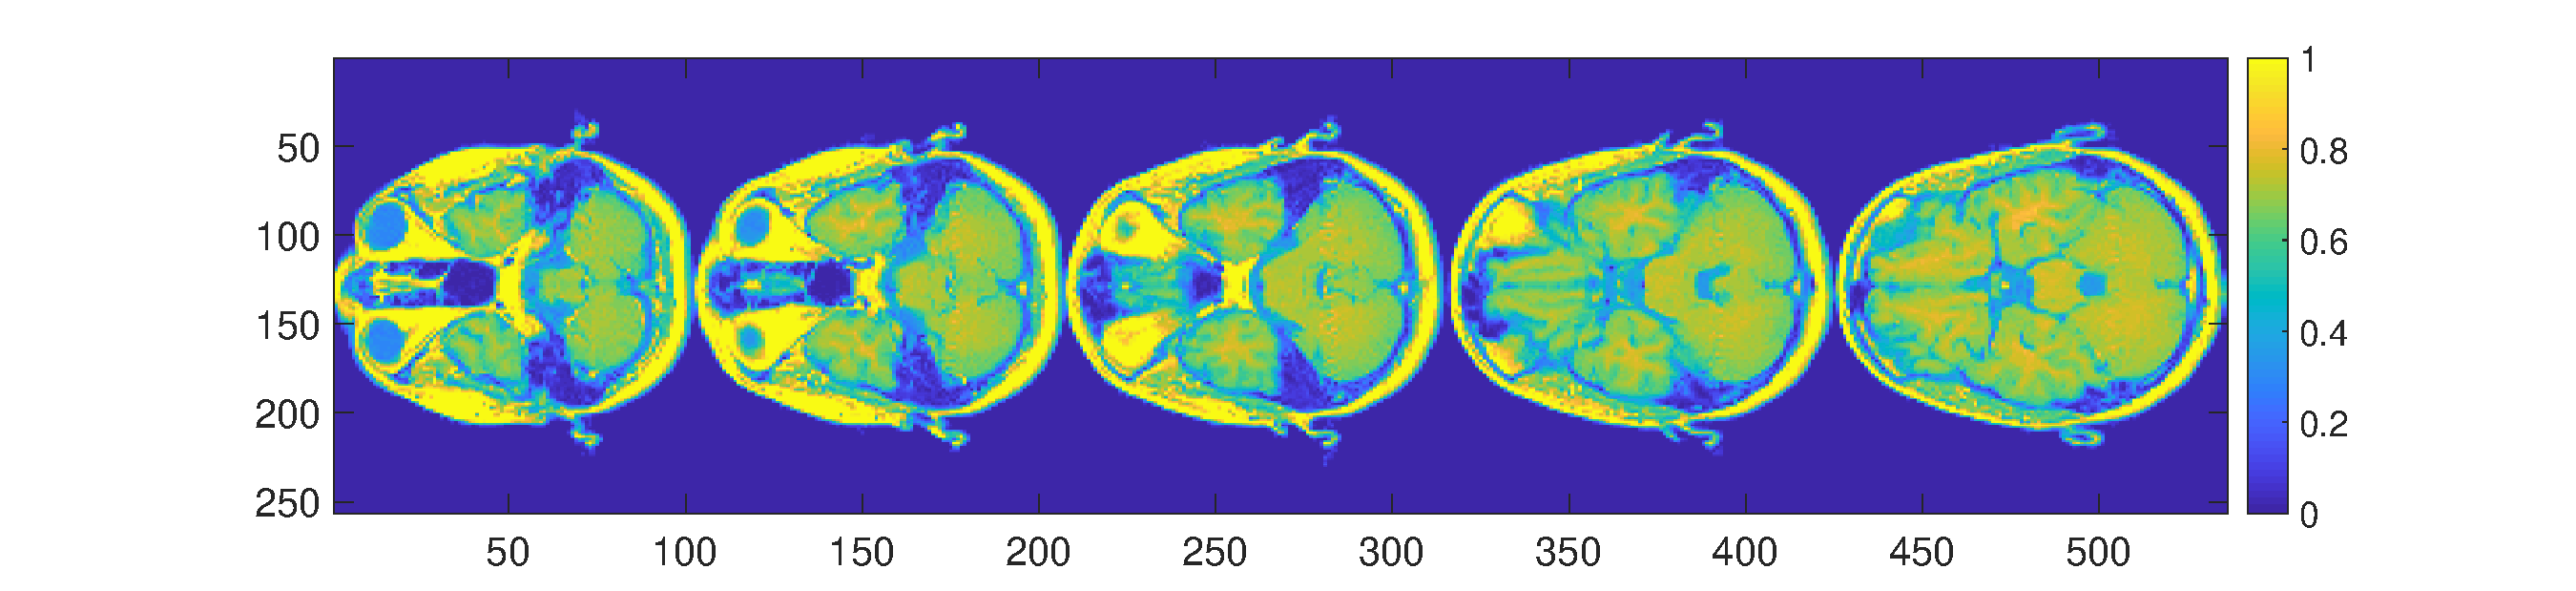
\includegraphics[scale=0.36]{Figures/Full_MRI}
\subcaption{}
\label{fig:MRI 1D True}
\end{subfigure} \\
\begin{subfigure}{\textwidth}
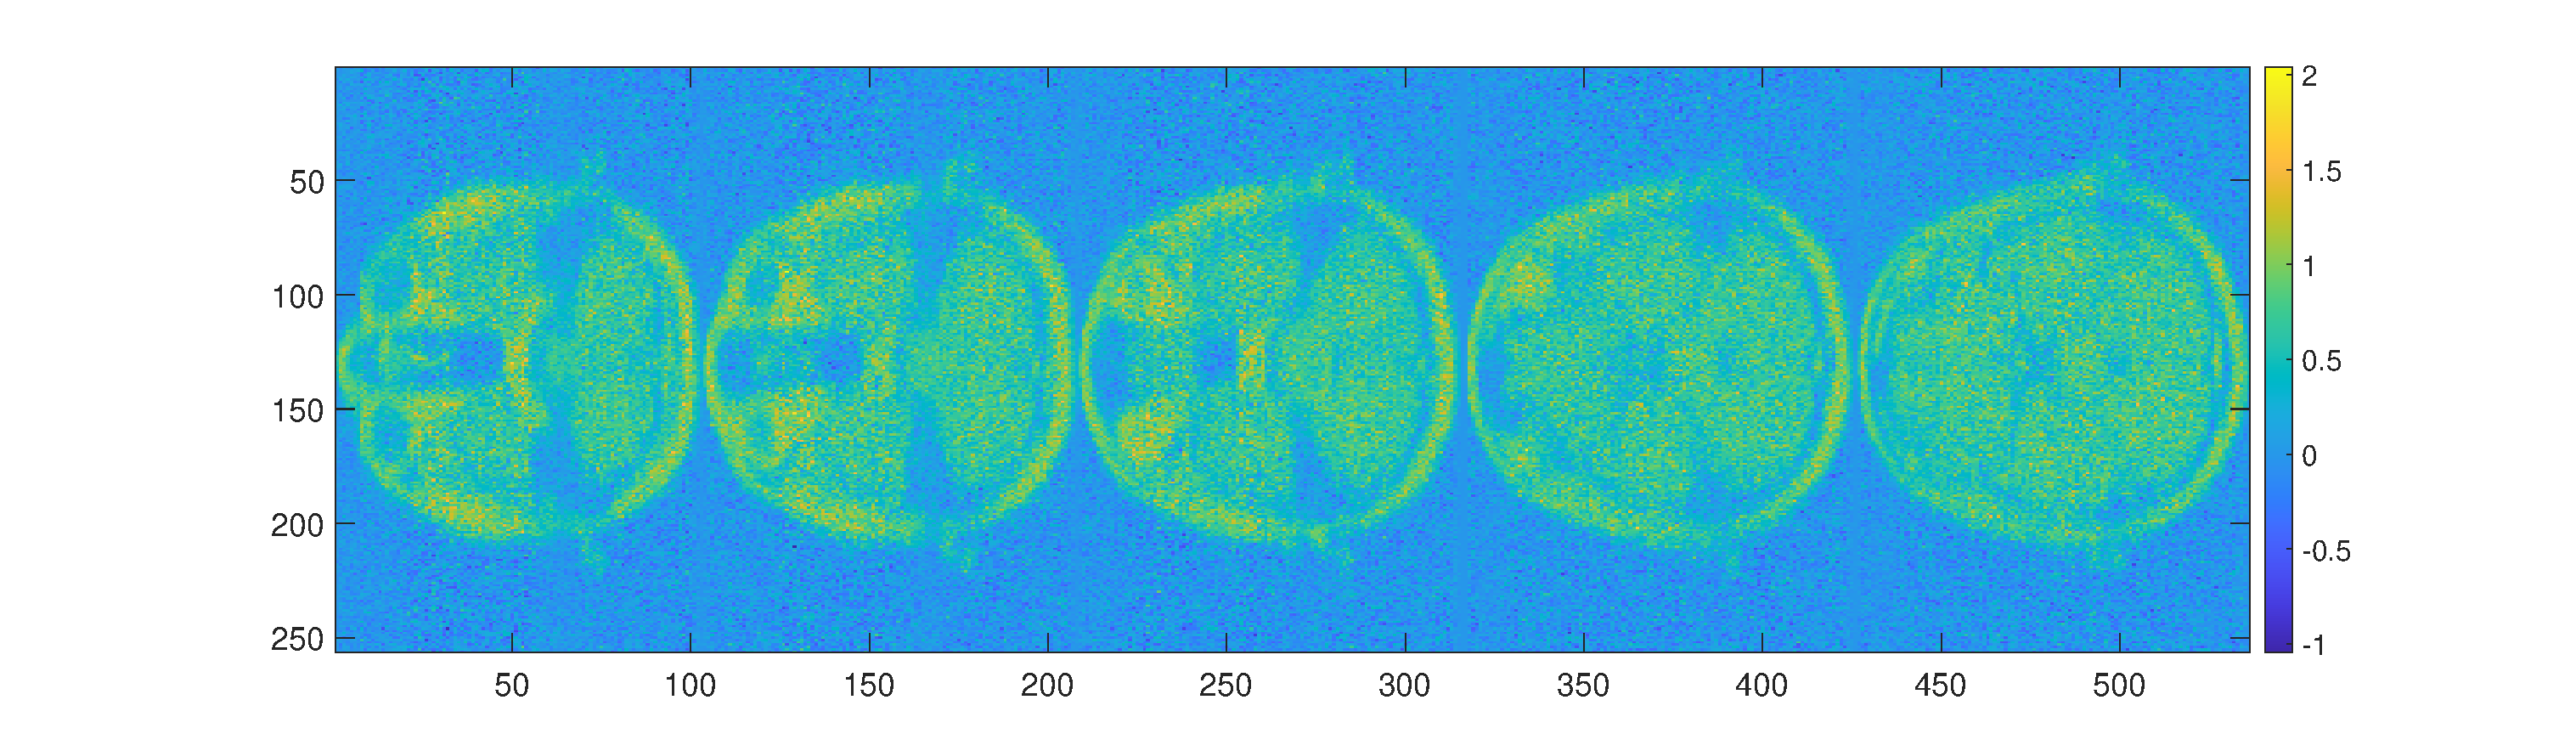
\includegraphics[scale=0.36]{Figures/Noisy_MRI}
\subcaption{}
\label{fig:MRI 1D Noisy}
\end{subfigure}
\caption{MRI data formed by reformatting the MATLAB built-in MRI data. Figure \ref{fig:MRI 1D True} shows the true data from which the training and validation vectors were selected. Each vector was blurred using a Gaussian kernel and normal noise was added; the resulting vectors are shown in Figure \ref{fig:MRI 1D Noisy}. The dimension of both images is $256 \times 536$.}
\label{fig:MRI 1D}
\end{figure}

\noindent The default dimension of each horizontal MRI slice accessible using \texttt{load mri.mat} is $128 \times 128$. Linear interpolation was used to double the number of rows; the number of columns of the concatenated MRI slices was trimmed to to eliminate leading and trailing zero columns. The columns of the image were then multiplied by a symmetric Toeplitz matrix, approximating a Fredholm integral equation of the first kind with a Gaussian kernel of mean 0 and variance 1 (each pixel representing a unit square in the continuous problem). The resulting MRI image is vertically blurred; see Figure \ref{fig:MRI 1D Noisy}. SNR values were selected randomly between 6 and 7 for each blurred column, and realizations of normal noise with the corresponding variances were added to blurred columns. The first $536/2 = 268$ columns of Figure \ref{fig:MRI 1D True} served as the training set, while the remaining 268 columns serve as a validation set.  The following $257 \times 256$ penalty matrix $L_1$ was used, which represents an approximation of a first derivative operator:
\[L_1 = \begin{bmatrix}
1 & & & \\
-1 & 1 & &  \\
 & \ddots &  \ddots & \\
 & & -1 & 1 \\
 & & & -1
\end{bmatrix}.\]
$L_1$ is the same penalty matrix used in \cite{ChungEspanol2017}. The resulting system matrix in \eqref{eq:TikSol3} has full column rank, and so applying the normal equations in terms of the GSVD results in unique solutions. \par 
Figure \ref{fig:Parameters 1D MRI} illustrates a comparison of the methods in terms of the regularization parameters $\regparam$ selected as the number of training vectors increases. 

\begin{figure}[ht]
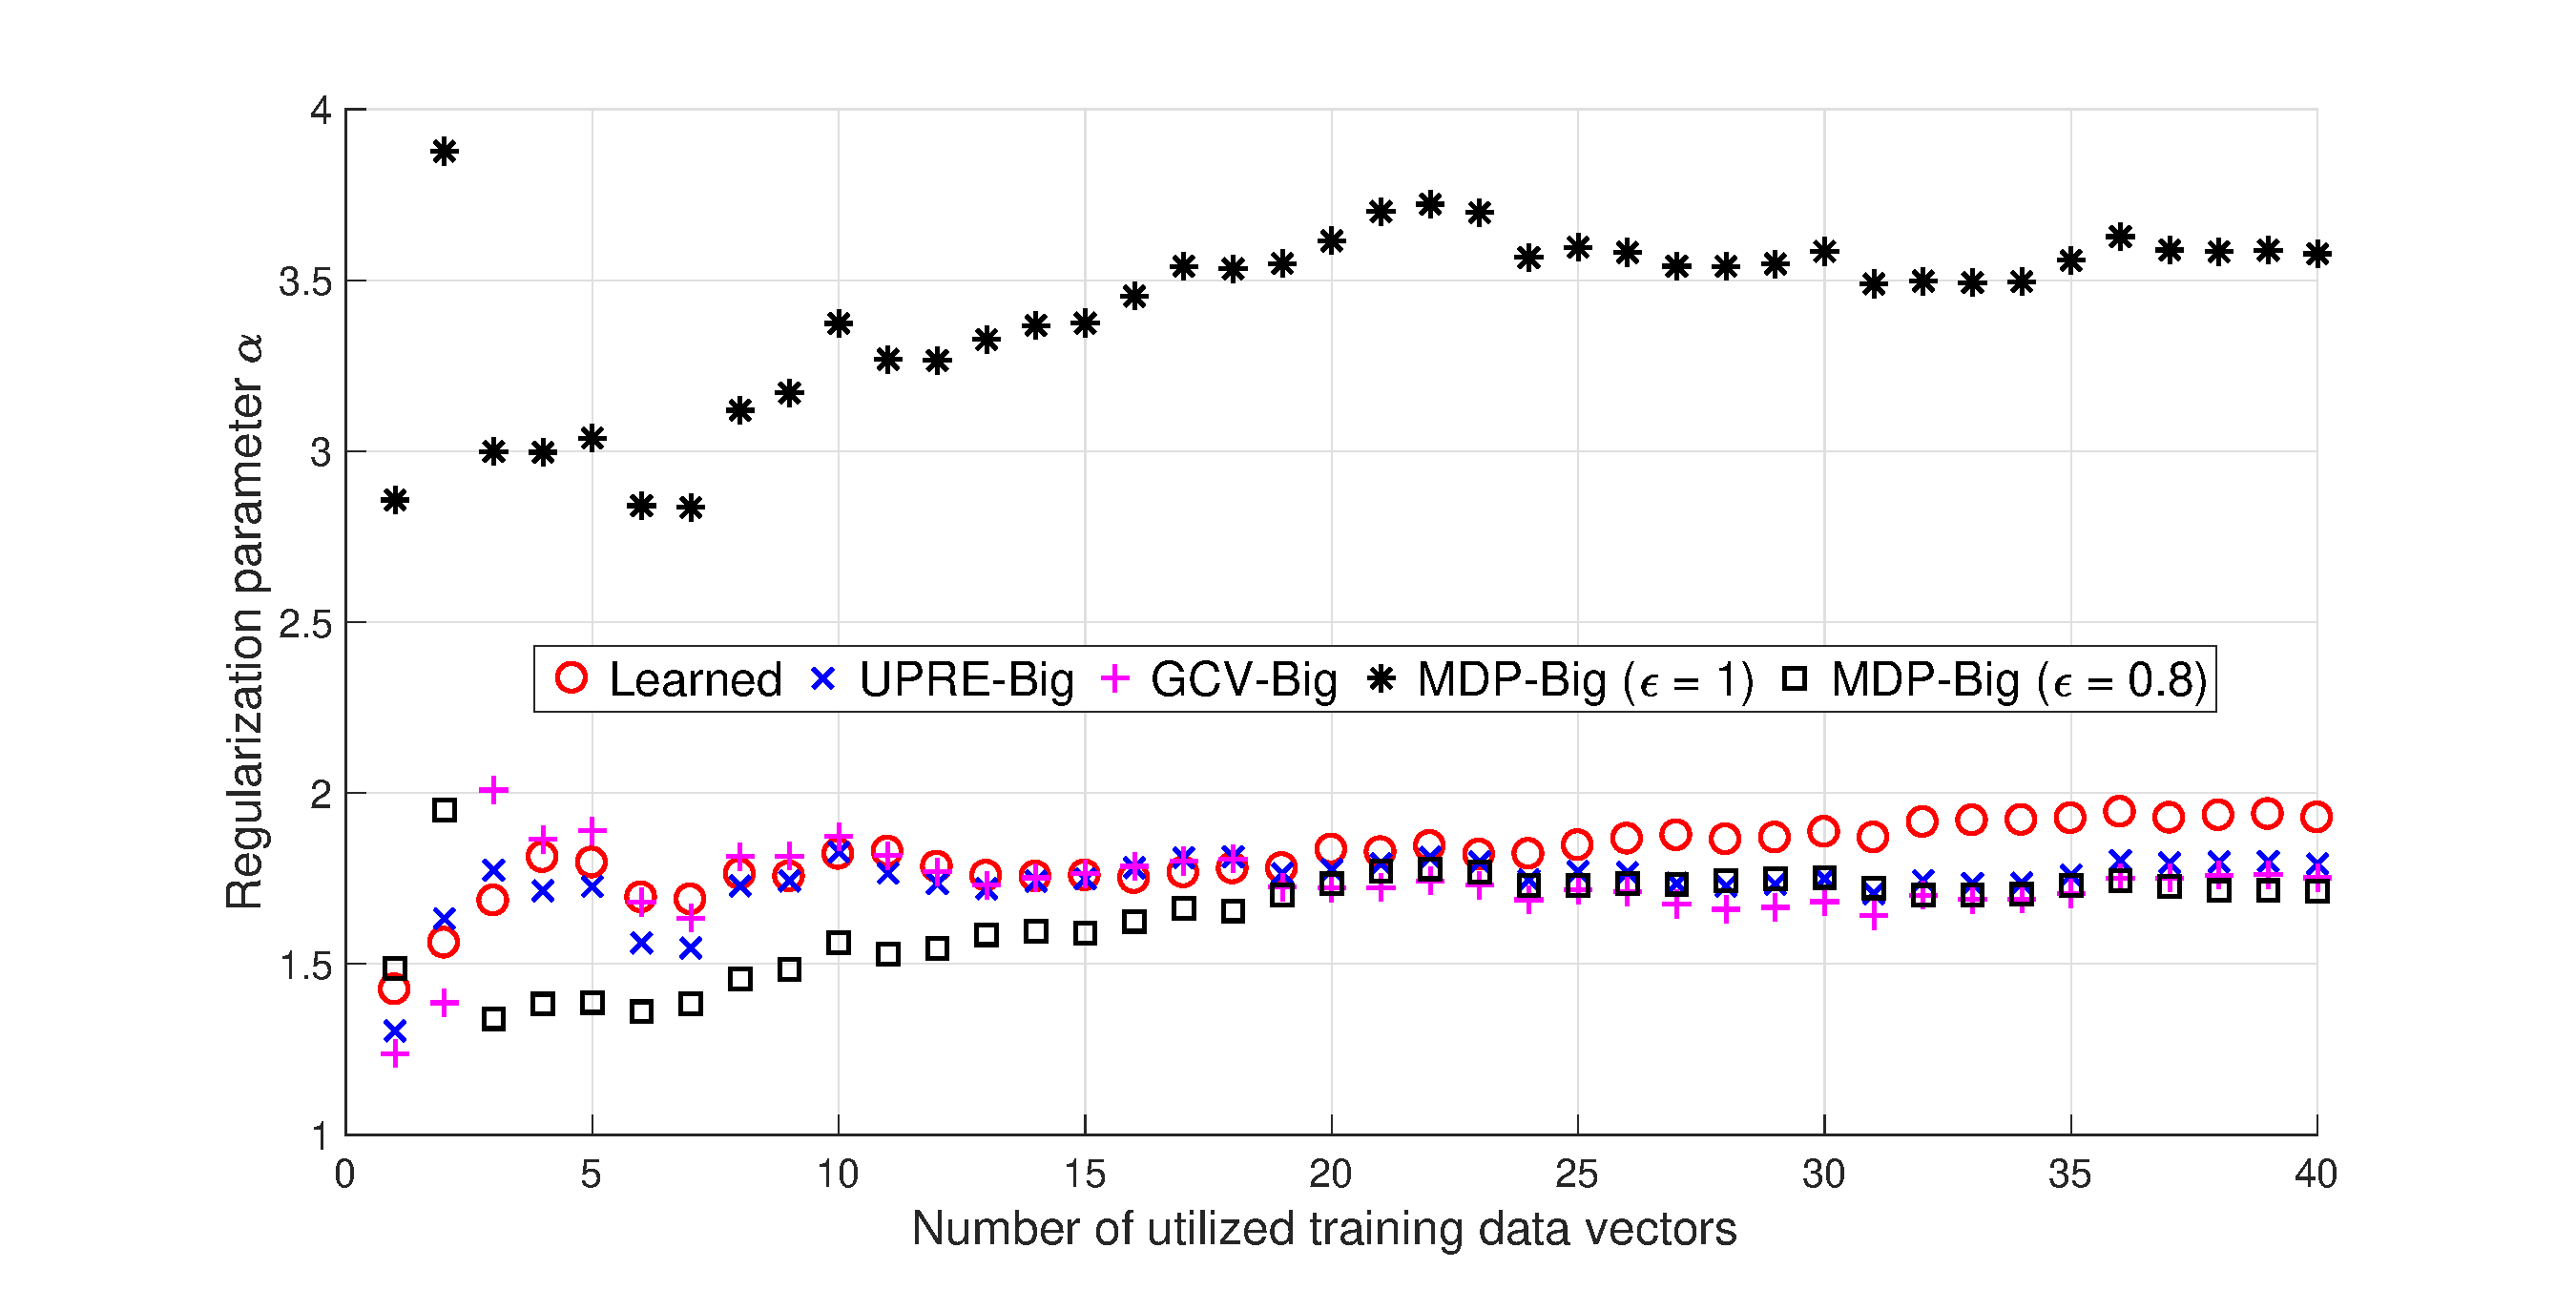
\includegraphics[scale=0.36]{Figures/Parameters1D_mri}
\caption{Trend of parameters selected by each adapted method as the number of training vectors increases. Note that the parameters essentially stabilize by about 40 training vectors out of the possible 268.}
\label{fig:Parameters 1D MRI}
\end{figure}

\noindent When the number of training vectors is small (e.g. between 1 and 10 from Figure \ref{fig:Parameters 1D MRI}), the parameters selected by all four methods change significantly. This can be attributed to the fact that all of the methods select a parameter that is either a root or a minimum of an average of functions. For a small amount of training vectors, each additional vector has more influence over the behavior of the adapted function. The parameters do seem to stabilize as the number of training vectors reach a certain point; in the problem being considered here, the parameters stabilize by about 40 training sets. The stabilization of the parameter most likely follows from the fact that each vector is part of the same type of image (MRI). It would seem unreasonable to expect the same stabilization when using vectors pulled from dissimilar images. \par 
Before looking at the relative errors of the regularized solutions, another observation regarding Figure \ref{fig:Parameters 1D MRI} can be made. While the parameters selected using the learning function \eqref{eq:Learning function} and the adapted UPRE and GCV methods are close (the maximum difference in the parameters does not exceed 0.5), the adapted MDP method consistently selected significantly larger parameters. A direct consequence is that the regularized solutions have higher relative errors. \par
Figure \ref{fig:Errors 1D MRI} shows the relative errors of the regularized solutions corresponding to the parameters from each method. 

\begin{figure}[ht]
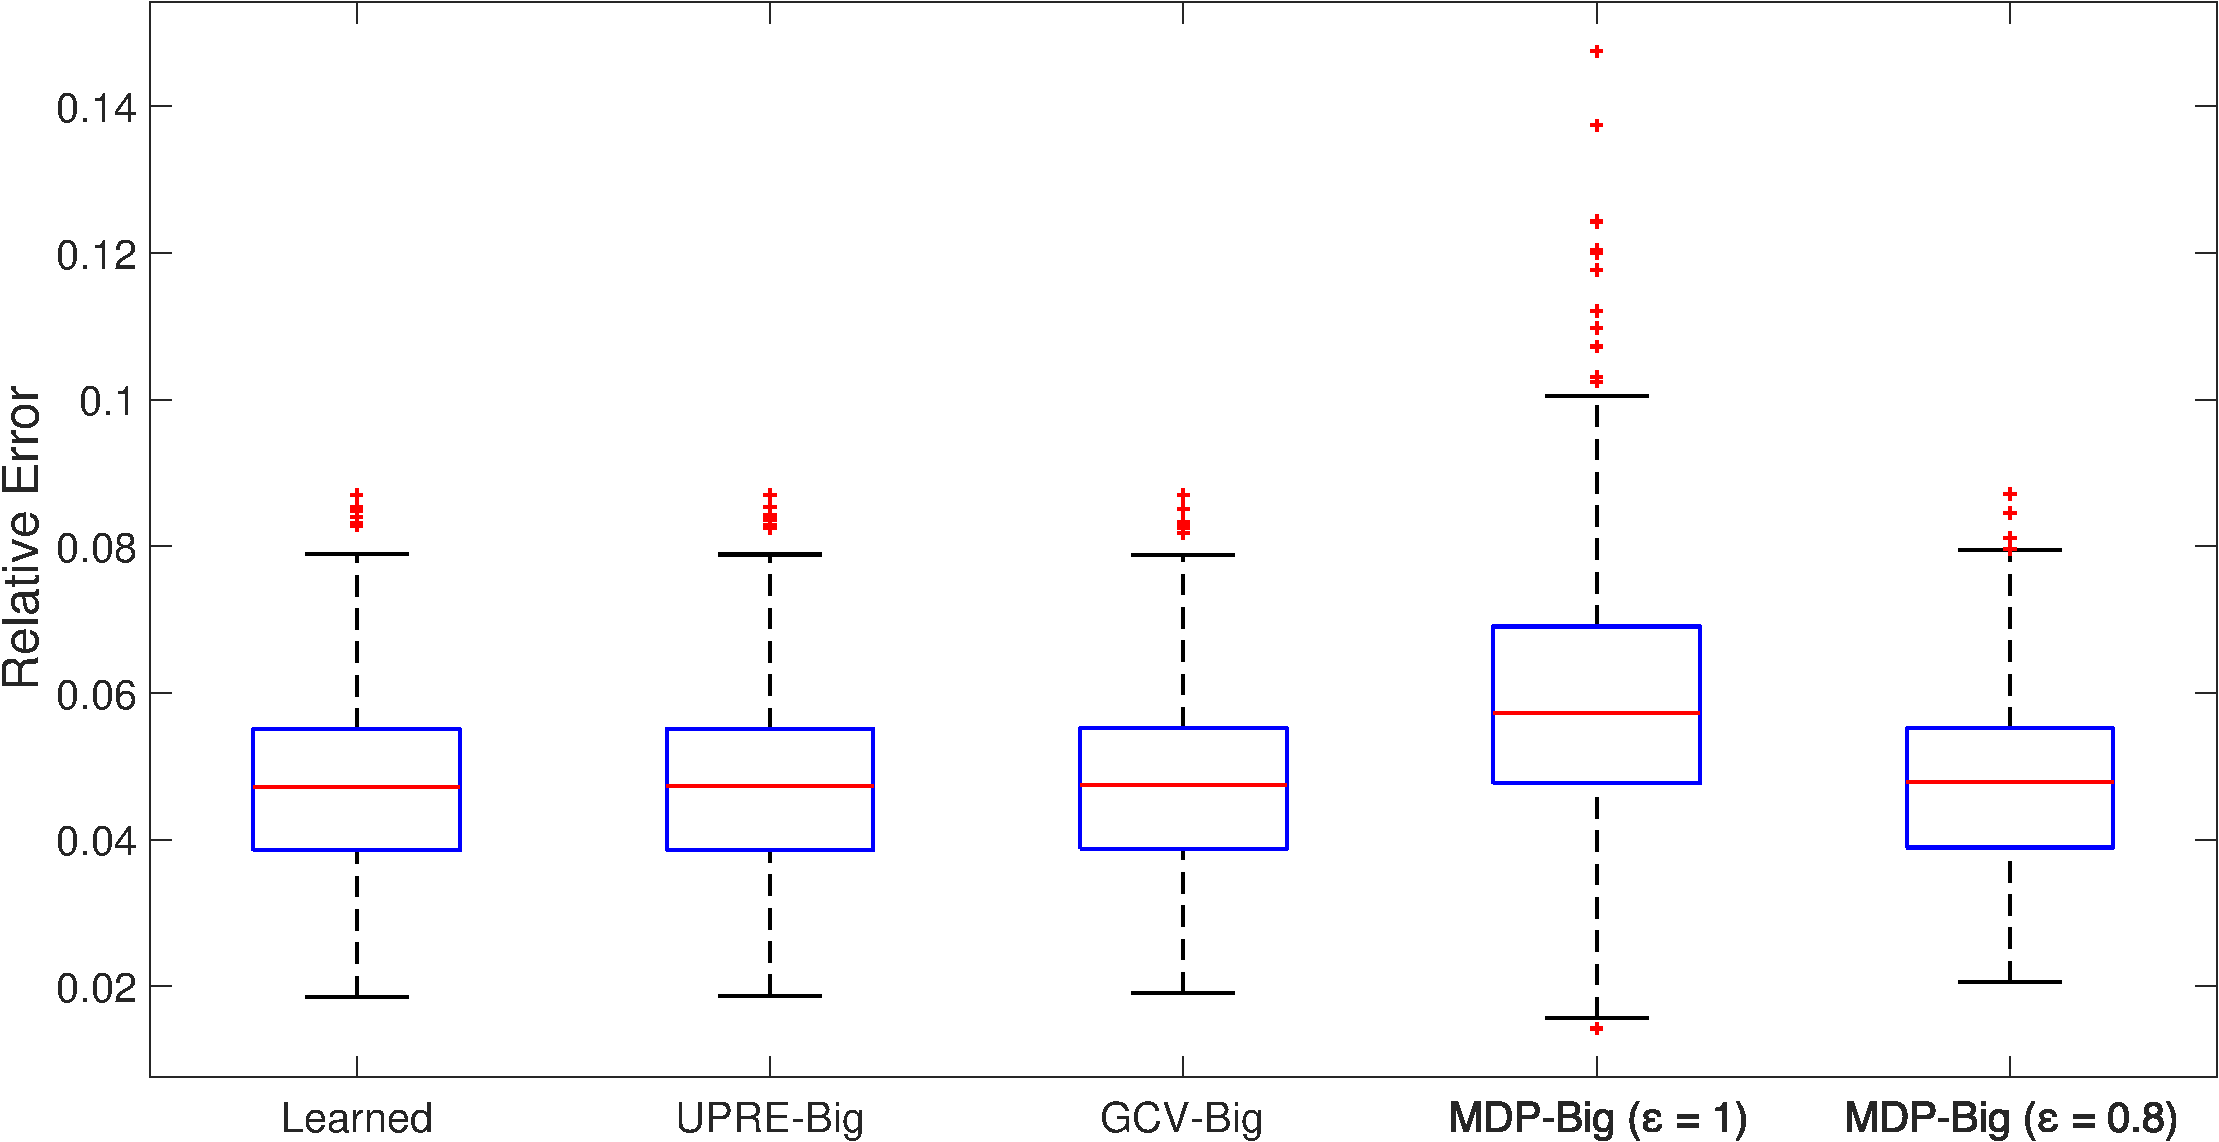
\includegraphics[scale=0.36]{Figures/Errors1D_mri}
\caption{Boxplots of the relative errors of each regularized solution versus the validation set. A parameter was selected using the full training set for each method, and the parameters of each method were used to generate regularized solutions from the validation set.}
\label{fig:Errors 1D MRI}
\end{figure}

\noindent Instead of using a relatively small amount of training vectors, like 40 out of 268 in Figure \ref{fig:Parameters 1D MRI}, the full training set was used to select a parameter from each method. These four parameters were then used to generate a regularized solution for each vector in the validation set, and the relative errors were computed against the true solutions. First, the relative errors obtained by the learning method and adapted UPRE and GCV methods are quite similar; the means of the relative errors are close, and there is a collection of upper outliers. In contrast, the adapted MDP method has a slightly larger mean relative error. However, the most striking visual characteristic from Figure \ref{fig:Errors 1D MRI} is the number of outliers in the MDP relative errors. The largest relative error obtained using the adapted MDP method is about twice the largest relative error of the other three methods. \par 
The one-dimensional test problem demonstrates that the adapted methods have potential for selecting viable regularization parameters that can be applied to multiple sets of data. The adapted UPRE and GCV performed competitively against the learning method, which relies on knowledge of the true training solutions. As stated previously, the success of the adapted methods is predicated on the similarity of the data sets being considered. However, this is not an unreasonable condition because data from a given experiment would hopefully vary little without significant change in the experimental set-up.

\subsection{Two-dimensional problems} \label{sec:2D}
The two-dimensional test problem again uses the MRI data built into MATLAB. However, the data sets now consist of image of size $256 \times 256$. A total of 20 default MRI images were used and split into training and validation sets containing 10 images each. For each MRI image, seven more images were generate through the use of random rigid transformations (rotations and translations) so that the training set and validation set each contained 80 images. A rotation angle $\theta$ and a translation angle $\phi$ were selected randomly between 0 and $2\pi$. Another scalar $c$ was drawn randomly between 0 and 64 so that the translation vector $\tVec = \trans{[c\cos(\phi),c\sin(\phi)]}$ does not have a magnitude that exceeds 64 pixels. Figure \ref{fig:MRI Transformations} shows examples of true MRI images used in the training set. 

\begin{figure}[ht]
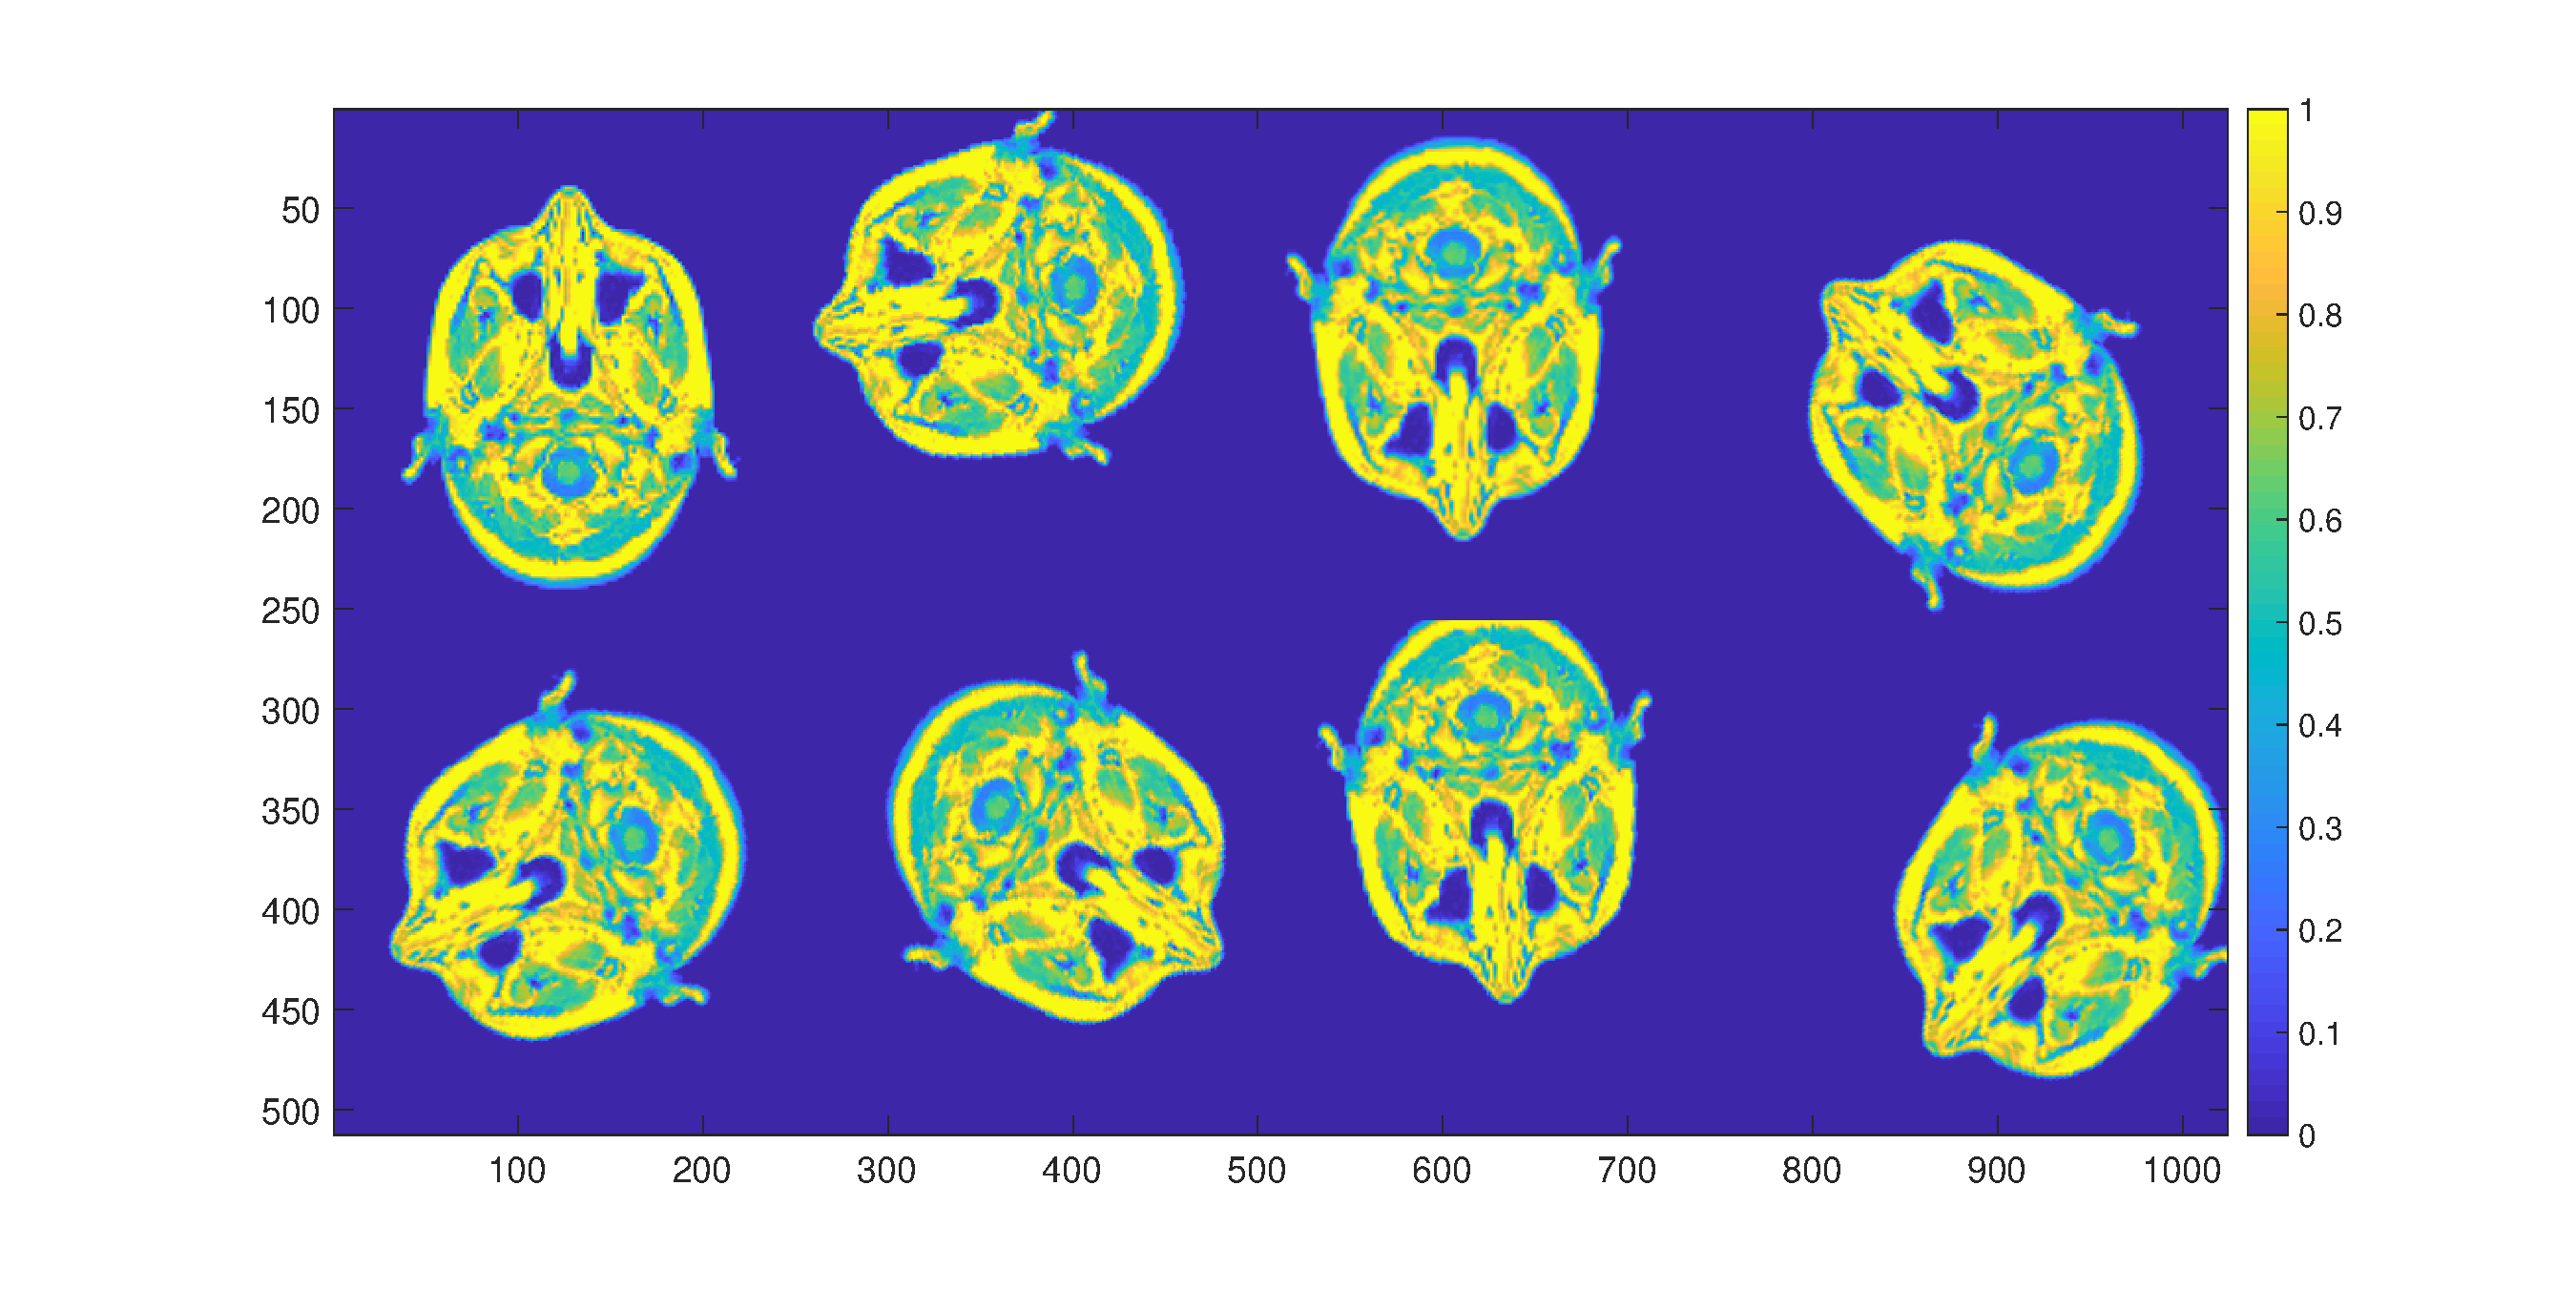
\includegraphics[scale=0.36]{Figures/MRI_Transformations}
\caption{Eight examples of true versions of training MRI images, each of size $256 \times 256$. The top left image is a default MRI image, while the remaining seven were generated from random rigid transformations. Nearest-neighbor interpolation was used when transformed pixel locations did not align with the rectangular grid.}
\label{fig:MRI Transformations}
\end{figure}

Circularly convolution of each image with a Gaussian kernel of mean 0 and variance 1 in each direction was then carried out to blur the images. Lastly, SNR values were randomly selected between 8 and 10 and realizations of normal noise with corresponding variance were added to the blurred images. \par 
Since circular convolution was utilized, the DFT was the primary tool for this MRI test problem as opposed to the GSVD. To ensure simultaneous diagonalization of the block system matrices $A$ and $L$, periodic boundary conditions were assumed so that both $A$ and $L$ are block-circulant-with-circulant-blocks (BCCB); see \cite{NeumannDCT,Vogel:2002}. The penalty matrix $L$ was selected to be the BCCB version of the discrete negative Laplacian operator, which is an approximation of the continuous Laplacian operator \cite{DebnathMikusinski2005,LeVeque2007}. The BCCB structure of $A$ and $L$ allows for simultaneous diagonalization using two-dimensional DFT for numerical efficiency. \par 
Figure \ref{fig:Parameters 2D} shows the parameters selected using each method. 
\begin{figure}[ht]
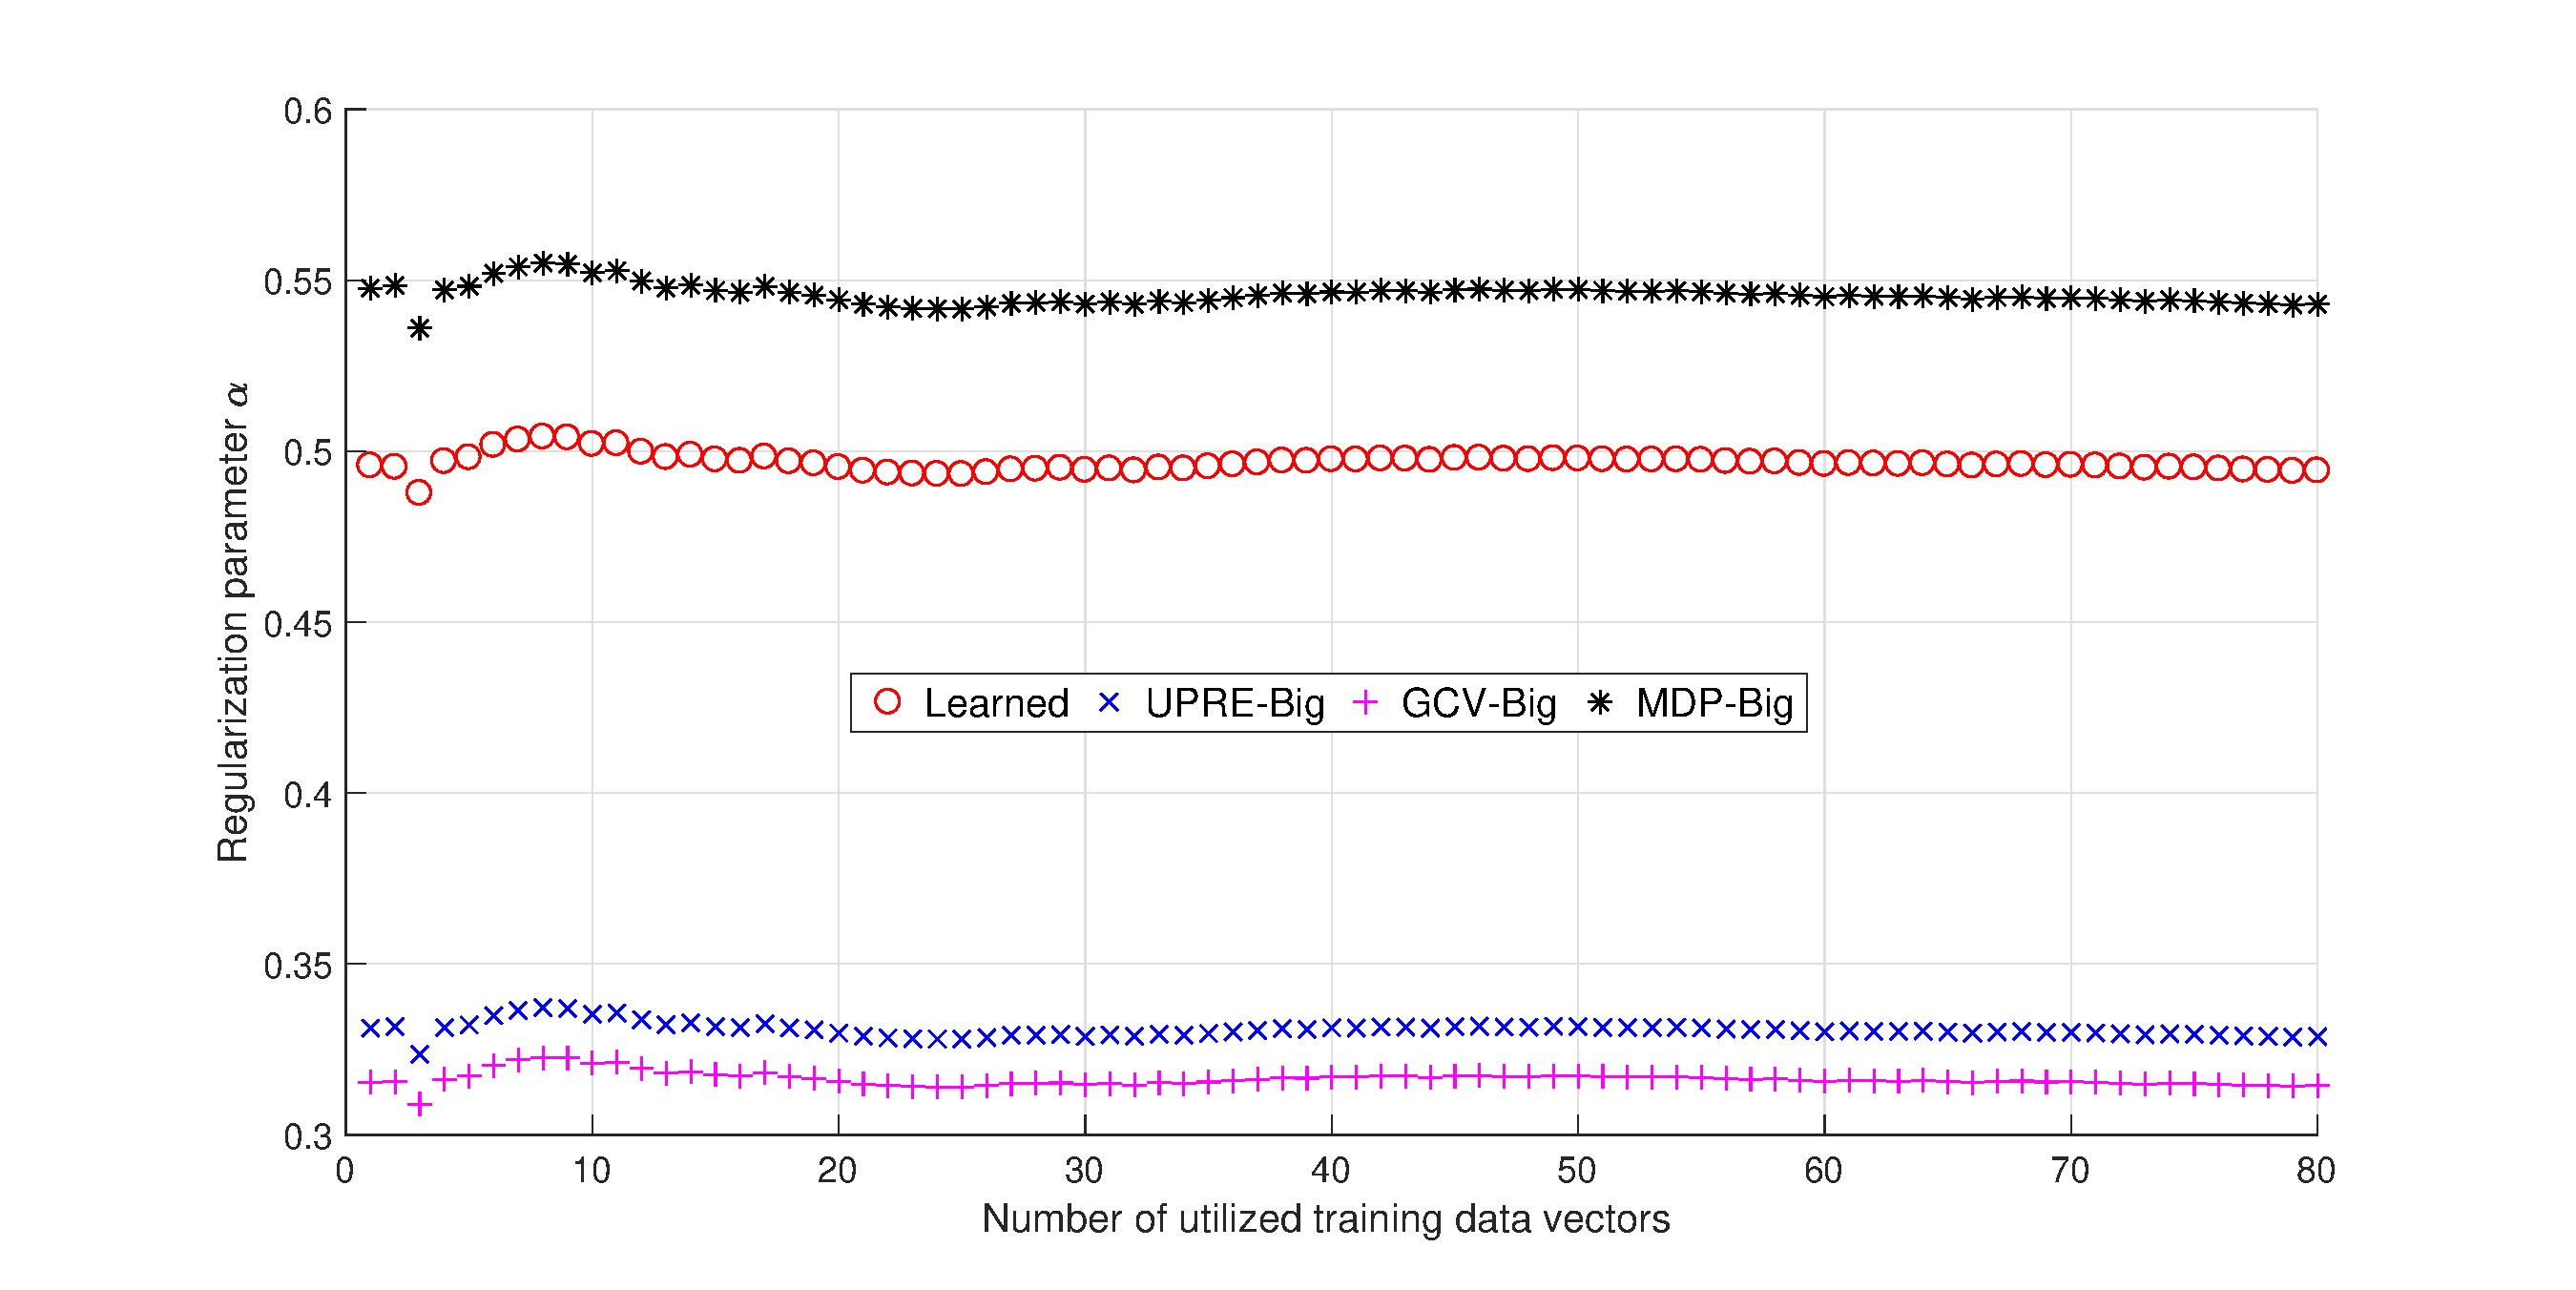
\includegraphics[scale=0.36]{Figures/Parameters2D_mri}
\caption{hello}
\label{fig:Parameters 2D}
\end{figure}
In contrast to the one-dimensional case, the adapted MDP method returned parameters closest to the parameters chosen based on the machine learning method. The adapted UPRE and GCV method selected parameters similar parameters. Another observation from Figure \ref{fig:Parameters 2D} is that the parameter obtained from each method are stable with respect to the number of images considered. This suggest that only small subset of the training set is needed to obtain regularization parameters that can be then applied to a full validation set. Figure \ref{fig:Errors 2D} contains boxplots of the relative errors of the regularized solutions for the validation set using 10 training images. 
\begin{figure}[ht]
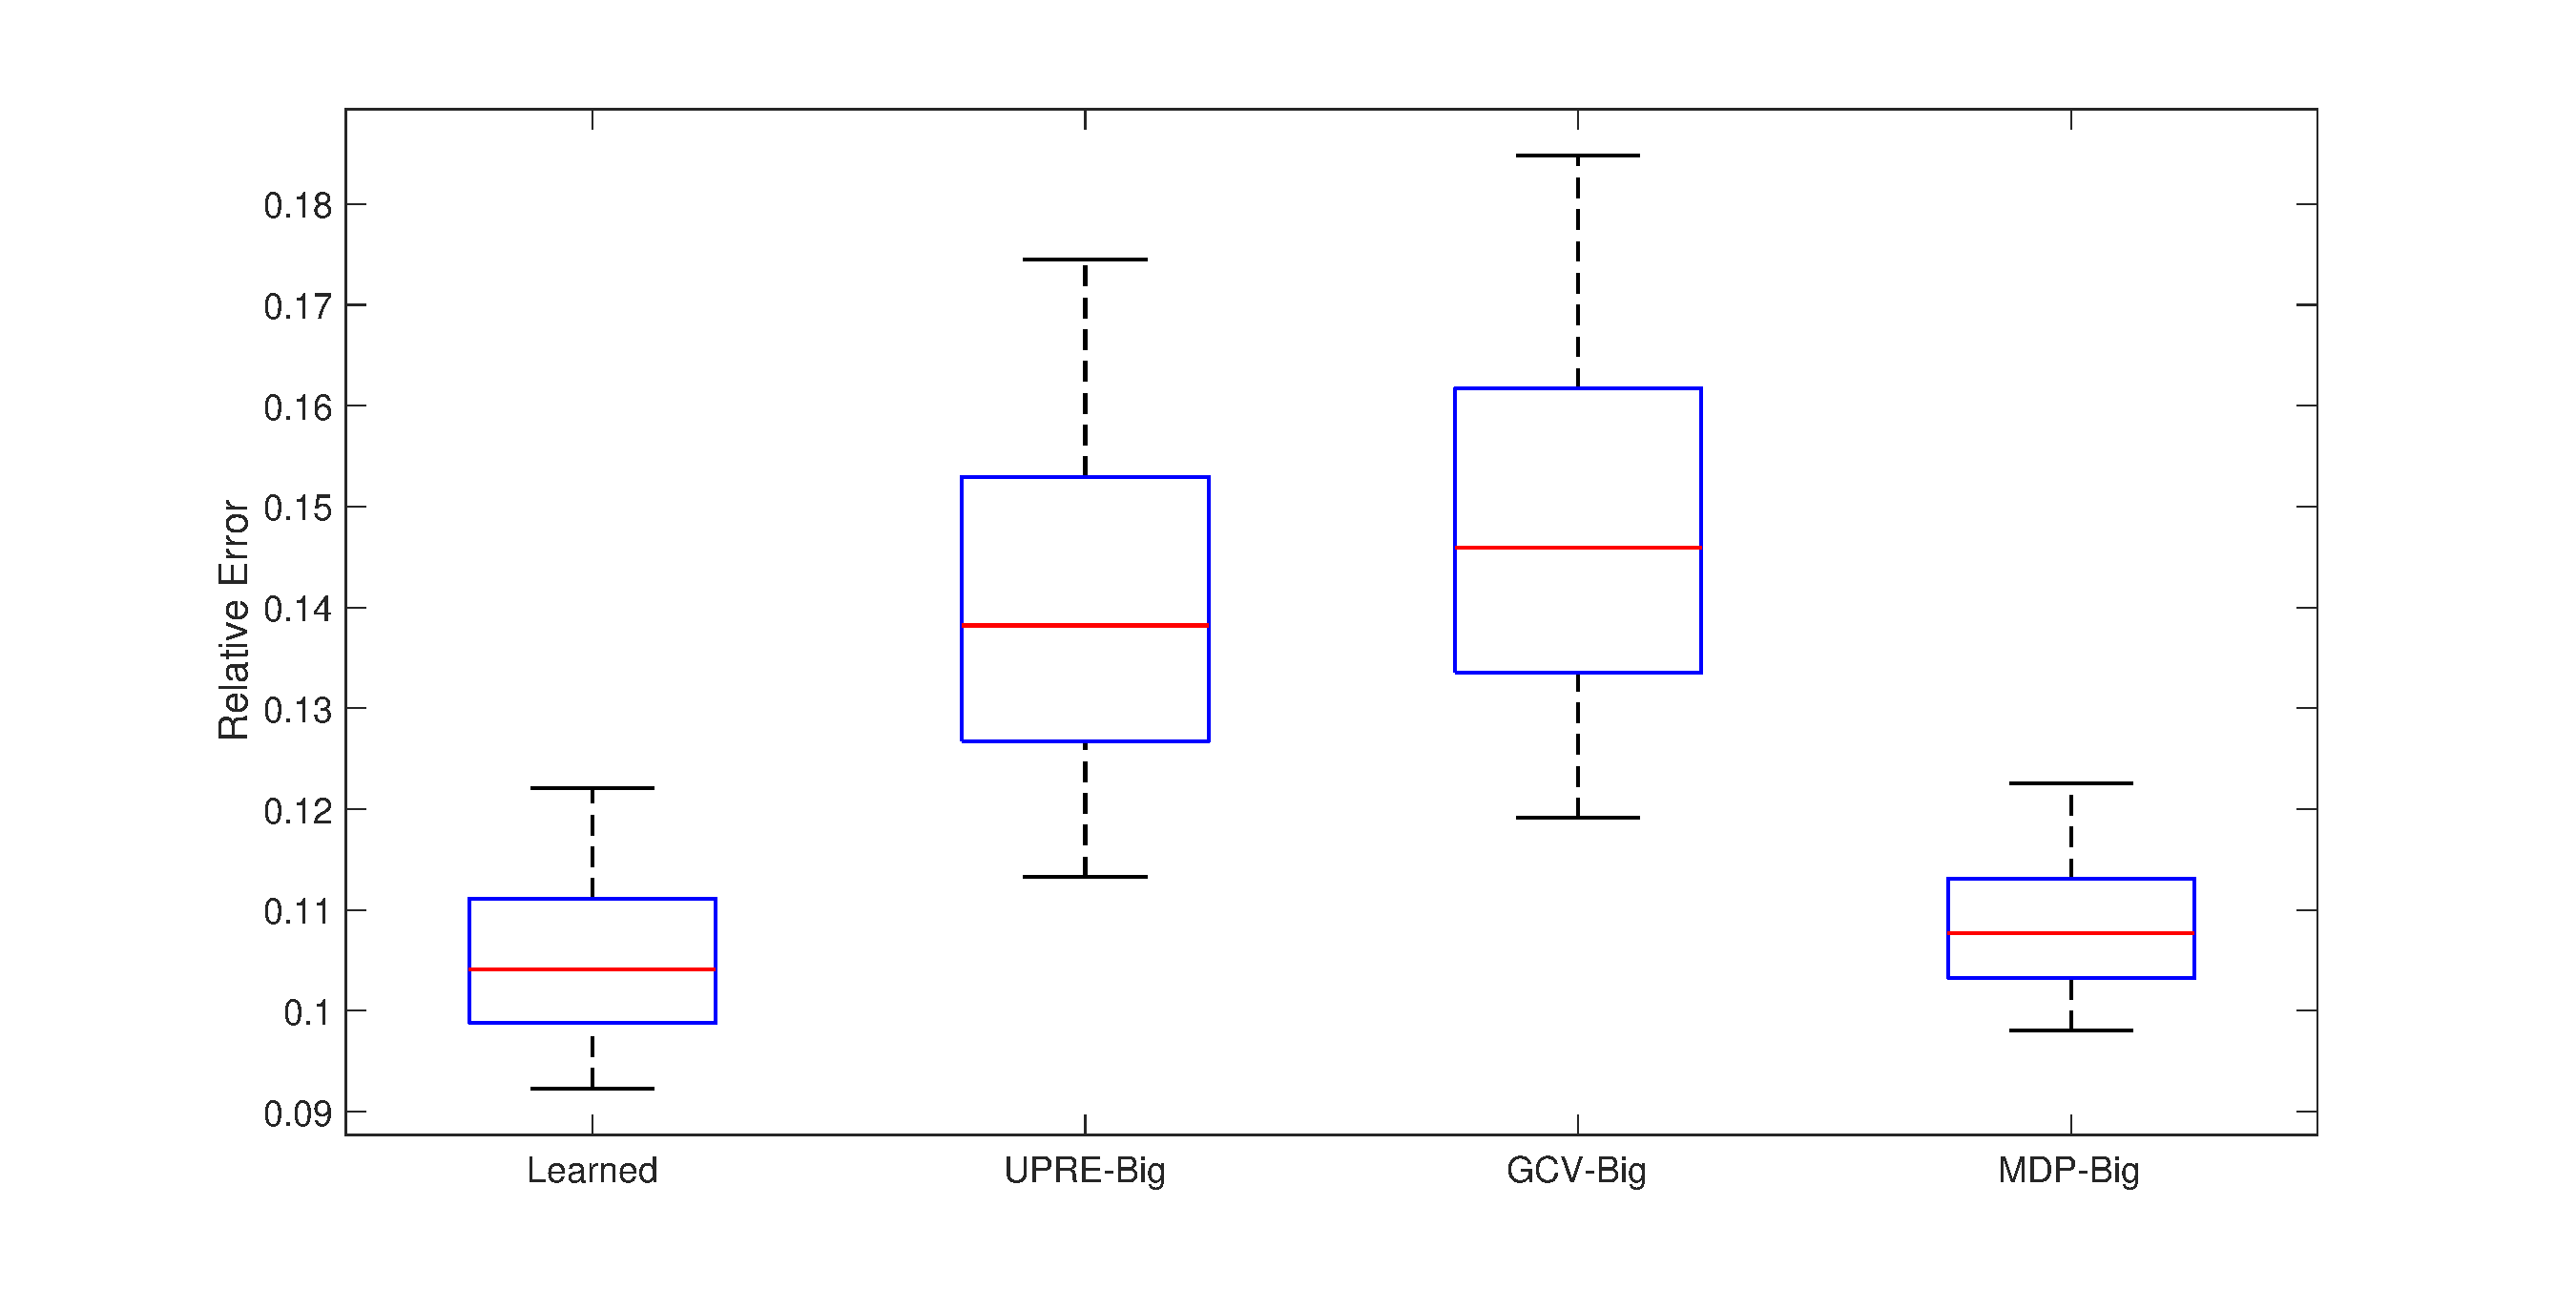
\includegraphics[scale=0.36]{Figures/Errors2D_mri}
\caption{hello}
\label{fig:Errors 2D}
\end{figure}
The errors of the regularized solutions obtained using the adapted MDP method are close to those of the machine learning method.

\begin{figure}
\label{fig:MESSENGER True}
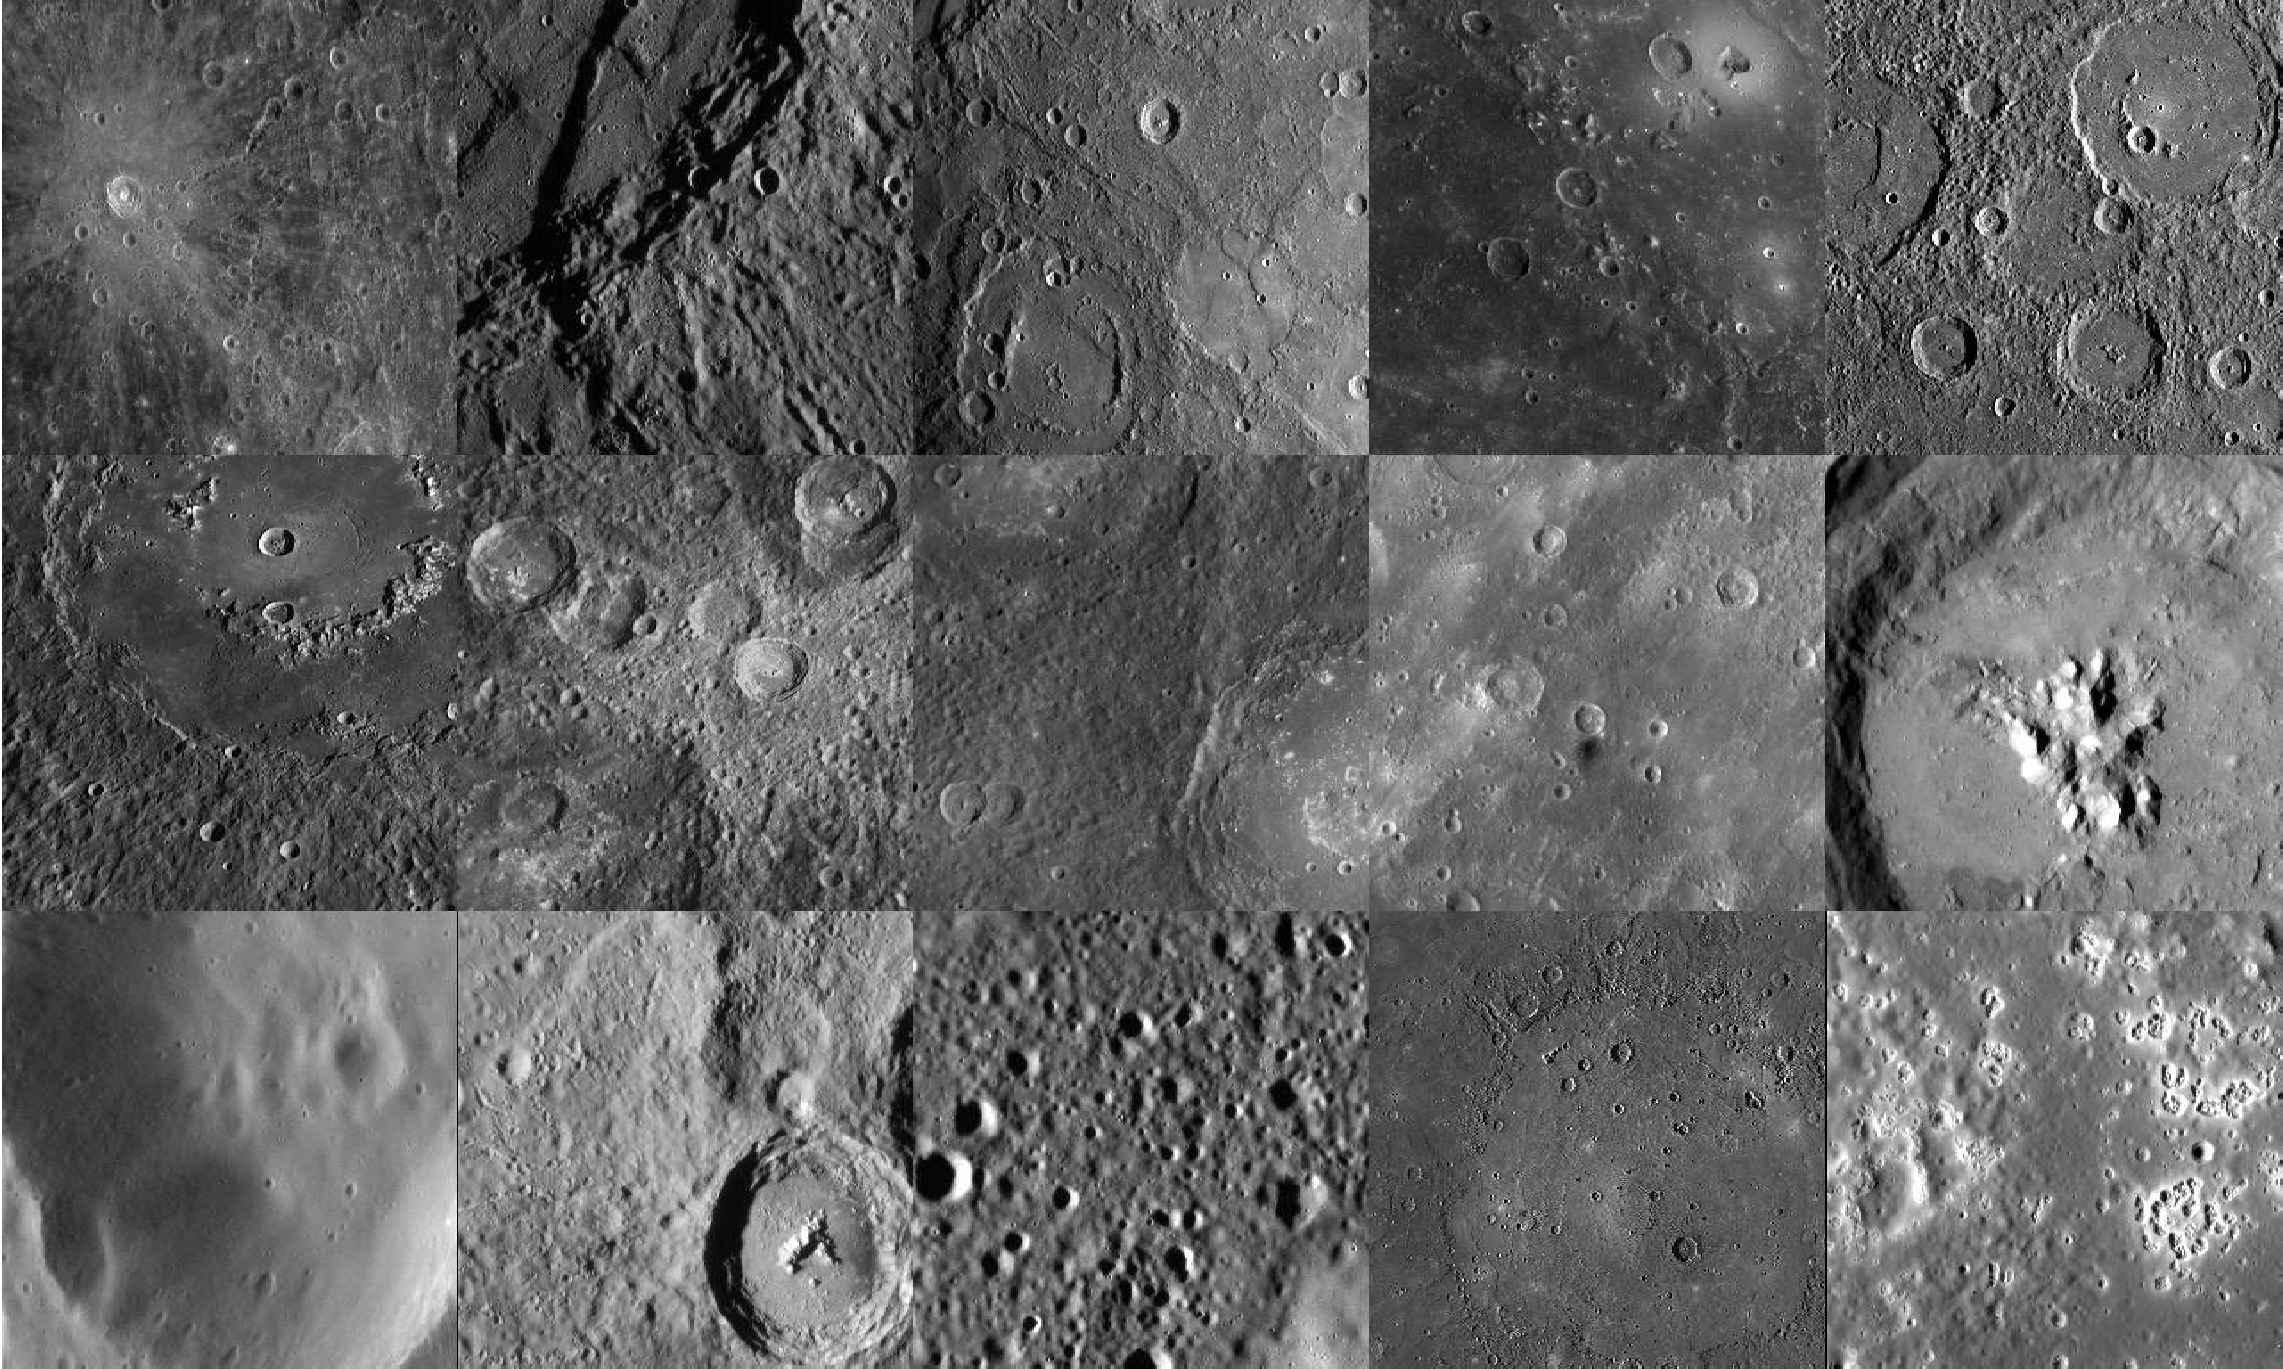
\includegraphics[scale=0.36]{Figures/MESSENGER}
\caption{Courtesy NASA/JPL-Caltech.}
\end{figure}

\section{Conclusions and future work} \label{sec:Conclusion}
In conclusion, this paper demonstrate a means by which UPRE, MDP, and GCV methods can be extended to accommodate multiple data sets. The most general forms of functions associate with these methods are \eqref{eq:UPRE 3}, \eqref{eq:Big MDP}, \eqref{eq:GCV Big}, and , respectively. The adapted UPRE and MDP methods are novel in that their corresponding functions can be written as an average of the individual functions associate with each data set. None of the three adapted methods require knowledge of true solutions unlike the machine learning approach defined by \eqref{eq:Learning function}, though the MRI test problems demonstrate that the adapted methods can perform competitively. \par
There are various directions of future investigation. Perhaps the most significant results could be obtained through approaches of determining the necessary number of data sets for a stabilization of selected parameters. Figure \ref{fig:Parameters 1D MRI} and Figure \ref{fig:Parameters 2D} suggest that obtained parameters stabilize fairly fast in relation to the number of data sets incorporate into the method functions. Another direction of future work would be to use the adapted methods on data sets containing images of differing objects. The MRI images used here are all visualizes of a human brain; it would be interesting to see how these methods perform for drastically different data sets.

\bibliographystyle{siam}
\bibliography{Parameter-Estimation}

\end{document}
